% Version 2006-12-05
\documentclass[12pt,glossary]{dalcsthesis}

% Definitions, Theorems, Lemmas, etc.
\newtheorem{definition}{Definition}
\newtheorem{theorem}{Theorem}
\newtheorem{lemma}{Lemma}

% A simple proof environment
\newenvironment{proof}{\paragraph{Proof.}}
{\nopagebreak\hfill\nopagebreak\rule{2mm}{2mm}\par\bigskip}
\usepackage[noend]{algpseudocode}
\usepackage{algorithm} 
\usepackage{graphicx}

%\usepackage[dvips]{graphicx}
\usepackage{subfigure}
\usepackage{lipsum}%
\usepackage[]{siunitx}
\usepackage{verbatim}
\usepackage{url}
\usepackage{rotating}
%\usepackage{makeidx}
\usepackage{enumitem}
%\usepackage[toc,page]{appendix}
%\usepackage{appendix}
%%for adding the code to appendix
%\let\cleardoublepage\clearpage

%\usepackage{breqn} %automatic line breaking
% after removing breqn, the minus symbol in the appendix code can be shown
\usepackage{listings}

\let\origlstlisting=\lstlisting
\let\endoriglstlisting=\endlstlisting
\renewenvironment{lstlisting}
    {\mathcode`\-=\hyphenmathcode
     \everymath{}\mathsurround=0pt\origlstlisting}
    {\endoriglstlisting}
\usepackage{color}    
\definecolor{pblue}{rgb}{0.13,0.13,1}
\definecolor{pgreen}{rgb}{0,0.5,0}
\definecolor{pred}{rgb}{0.9,0,0}
\definecolor{pgrey}{rgb}{0.46,0.45,0.48}
\lstset{%language=Java,
  showspaces=false,
  showtabs=false,
  breaklines=true,
  captionpos=b,
  %frame=single, 
  frame=L,
  numbers=left,
  numbersep=7pt,  
  numberstyle=\color{pgrey},
  tabsize=3, 
  showstringspaces=false,
  breakatwhitespace=true,
  extendedchars=true,
  commentstyle=\color{pgreen},
  keywordstyle=\color{pblue},
  stringstyle=\color{pred},
  basicstyle=\ttfamily,
  moredelim=[il][\textcolor{pgrey}]{$$},
  moredelim=[is][\textcolor{pgrey}]{\%\%}{\%\%}
}

%\let\cleardoublepage\clearpage 

%%for adding the code to appendix--done

%%%add by me
\usepackage[intoc]{nomencl}
\makenomenclature
\renewcommand{\nomname}{List of Abbreviation and Symbols Used}


%%added by me August 4th
% \usepackage[acronym]{glossaries}
% \makeglossaries
% \newacronym{abc}{ABC}{a sample acronym}
% \renewcommand*{\acronymname}{Abbreviations}

\begin{document}

\mcs  % options are \mcs, \macs, \mec, \mhi, \phd, and \bcshon
\title{Maritime Traffic Anomaly Detection from AIS Satellite Data in Near Port Regions}
\author{Bo Liu}
\defenceday{10}
\defencemonth{August}
\defenceyear{2015}
\convocation{October}{2015}

% Use multiple \supervisor commands for co-supervisors.
% Use one \reader command for each reader.

\supervisor{Dr. Stan Matwin}
\reader{Dr. Raza Abidi}
\reader{Dr. Ronald Pelot}

% \nolistoftables
% \nolistoffigures

\frontmatter



\begin{abstract}
%Maritime traffic monitoring is an important aspect of safety and security in close to port operations. While there is a large amount of data with variable quality, decision makers need reliable information about possible situations or threats. To address this requirement, we propose a two-component maritime traffic anomaly detection model in this thesis. First, it extracts normal ship trajectory patterns that builds clusters using, besides ship tracing data, the publicly available International Maritime Organization Rules. The main result of clustering is a set of generated lanes that can be mapped to those defined in the IMO directives. Since the normal extraction model also takes the attributes of speed and direction into account, the clustering results allow decision makers to detect abnormal patterns - vessels that do not obey the normal lanes or sail with higher or lower speeds.  Then, we show how the second anomaly detection component can detect anomalous navigational behaviors based on three specialized division distances with the clusters. It decides for each trajectory point if the vessel is anomalous, considering longitude, latitude, speed and direction. Although the approach is point-based, which is applicable for real-time AIS surveillance, it is also flexible enough for analysts to set their own threshold for labeling whole trajectories.
Maritime traffic monitoring is an important aspect of safety and security in close-to-port operations. While there is a large amount of data with variable quality, decision makers need reliable information about possible situations or threats. In this thesis, we propose a two-component maritime traffic anomaly detection model. First, it extracts normal ship trajectory patterns using, besides ship tracing data, the publicly available IMO Rules. The main result of clustering is a set of generated lanes that can be mapped to those defined in the IMO directives. Then, we show how the second anomaly detection component detects anomalous navigational behaviors based on three specialized division distances with the clusters. It decides for each point if the vessel is anomalous, considering longitude, latitude, direction and speed. This point-based approach is applicable for real-time AIS (Automatic Identification System) surveillance; it is also feasible for analysts to set their own threshold for labeling whole trajectories.

%Since the model also takes non-spatial attributes (speed and direction) into account, the results allow decision makers to detect abnormal patterns - vessels that do not obey the normal lanes or sail with higher or lower speeds.


\end{abstract}

\printnomenclature[3cm]
\nomenclature{SOG}{Speed Over Ground}
\nomenclature{COG}{Course Over Ground}
\nomenclature{GV}{Gravity Vector}
\nomenclature{SSP}{Sampled Stopping Point}
\nomenclature{AIS}{Automaitc Identification System}
\nomenclature{IMO}{Iternational Maritime Organization}
\nomenclature{TSS}{Traffic Separation Scheme Boundaries}
\nomenclature{GPS}{Global Positioning System}
\nomenclature{DBSCAN}{Density-Based Spatial Clustering of Applications with Noise}
\nomenclature{DBSCANSD}{Density-Based Spatial Clustering of Applications with Noise considering Speed and Direction}
\nomenclature{ADD}{Absolute Division Distance}
\nomenclature{RDD}{Relative Division Distance}
\nomenclature{CDD}{Cosine Division Distance}

%DTW
%PDF
%KDE
%GMM


%\printglossary
%\glossary{name={Preparation},description={Getting ready to do something}},
%\glossary{name={Preparation},description={Getting ready to do something}}


\begin{acknowledgements}

%To edit.
I would like to first express my deepest appreciation to my supervisor, Dr.Stan Matwin, for his support, guidance, encouragement and patience throughout my master program. His valuable suggestions and directions helped to improve the quality of this thesis. He also provides me with precious opportunities to work with multiple projects which can help me open my view.

Besides my supervisor, I would like to thank the rest of my thesis committee: Prof.Raza Abidi, Prof.Ronald Pelot and Prof.Dirk Arnold for their encouragement, insightful comments, and hard questions.

My sincere thanks also goes to Dr.Erico N.de Souza, my project leader. His advices and ideas guided me work on the right paths of the projects. He has also spent a lot time reviewing my papers and this thesis, which is a great help to me.

My parents, Baolong and Changling, who have always been supporting me and have never said no to my any decisions. Without them, this thesis cannot be finished.


I would also like to extend my gratefulness to all my friends and labmates in the Big Data Institute: Dr.Rob Warren, Dr.Xiaoguang Wang, Ahmad, Behrouz, Diana, Habibeh, Xuan, Eman, Baifan, David, Lulu and Vineeth for the stimulating discussions and for all the fun we have had in the past two years.

Last but not least, I would like to  acknowledge the generous support of GSTS, Inc., ExactEarth, Inc., Marine Environmental, Observation, Prediction And Response Network (MEOPAR), and the Natural Science and Engineering Research Council of Canada (NSERC).




\end{acknowledgements}

\mainmatter




\chapter{Introduction}





Today maritime transportation represents 90\% of international trade volume \cite{vespe12} and there are more than 50,000 vessels sailing the ocean every day \cite{Nicolas}. So the challenges related to safety and security aspects in the maritime domain are of high priority. 
Modeling ship behavior helps improve security for authorities and one crucial task of maritime surveillance is abnormal vessel behaviours detection.
Anomalies in the maritime domain, such as unexpected stops, deviations from regulated routes, inconsistent speed or direction etc., may be related to risks like collisions\footnote{http://gcaptain.com/tag/ship-collision/}, grounding\footnote{http://www.wisegeek.com/what-is-ship-grounding.htm}, sea drunkenness\footnote{http://www.theglobeandmail.com/news/national/canadian-navy-officer-charged-with-drunkenness-disobeying-orders/article23023966/},  smuggling, piracy\footnote{http://www.maritime-executive.com/article/pirates-attack-two-vessels-in-asia}, etc. To address the issue, different data sources such as data from Automatic Identification System (AIS), synthetic aperture radar, high frequency surface wave radars, infra-red sensors, videos and intelligent reports \cite{masterthesis} are used by the maritime authorities.   Data generated by AIS are utilized in this thesis. 

Automatic Identification System (AIS) is an automatic tracking system to identify and locate vessels by exchanging data with other nearby ships, AIS base stations and satellites. The use of this system has been required by the International Maritime Organization (IMO) since 2004 to enhance safety and efficiency of navigation and improve situational awareness and assessment \cite{AISHarati}. IMO was established in Geneva in 1948 with an initial name of Inter-Governmental Maritime Consultative Organization (IMCO). Then in 1982, it was changed to the International Maritime Organization \footnote{https://en.wikipedia.org/wiki/International\_Maritime\_Organization}. The IMO's headquarter is in London, United Kingdom and it is a specialised agency of the United Nations with 171 Member States and three Associate Members. IMO is the global standard-setting authority for the safety, security and environmental performance of international shipping \footnote{http://www.imo.org/en/About/Pages/Default.aspx}.
According to the regulations defined by IMO, all ships of 300 gross tonnage and upwards engaged on international voyages and cargo ships of 500 gross tonnage and upwards not engaged on international voyages and passenger ships irrespective of size shall be fitted with an automatic identification system and over 400,000 ships worldwide have installed these transponders \cite{AISdummies}. 

AIS messages are automatically broadcasted with a reporting frequency directly proportional to the speed of the vessel \cite{kde}.  The data can certainly be viewed as big data: a stream of some 80 million messages are generated per day. Two categories of data (static and dynamic information) are transmitted by the AIS transponders. Static information, which must be programmed into the AIS transceiver,  includes IMO number, Maritime Mobile Service Identity (MMSI)\nomenclature{MMSI}{Maritime Mobile Service Identity} number, vessel call sign, vessel type, vessel dimensions (length and beam). The dynamic information, which needs to be updated automatically, includes the ship's location (Longitude and Latitude), Course Over Ground (COG), Speed Over Ground (SOG), heading, Rate of Turn (ROT), time in UTC (Coordinated Universal Time)\nomenclature{UTC}{Coordinated Universal Time}, navigational status etc \cite{IALA}. In this thesis, both static and dynamic information is used to tackle the maritime anomaly detection task.


IMO also controls the navigational lanes that vessels must use when approaching some ports around the world. Specifically, the rules which regulate the general directions in the specific regions for the vessels to navigate are called Traffic Separation Schemes (TSS) \cite{tss}.  The regulations to establish TSSs mandatory were first proposed by IMO's Maritime Safety Committee meeting in March 1971 and this recommendation was adopted by the IMO later the same year. The first corresponding mandatory traffic scheme is the Dover Straits scheme.\footnote{http://www.imo.org/OurWork/Safety/Navigation/Pages/ShipsRouteing.aspx} These navigational lanes are definitely good resources for maritime surveillance analysis, but unfortunately, current tools do not offer automatic ways to check whether the vessels are obeying these lanes. 

Although TSS regulates the normal geographical lanes for ships to sail, it does not provide exact speed regulations in specific regions. More specifically, there are no rules to determine the maximum or minimum speed of a particular type of vessels to sail in a given area. As a consequence, only checking if the ships are obeying the lanes cannot satisfy the demand of maritime surveillance. Fortunately, one dynamic type of information, SOG (Speed Over Ground), is included in AIS messages and approaches that are able to utilize this historical speed information for anomaly detection are desirable.

%In this thesis, we first propose a clustering-based model that uses IMO rules in clustering real trajectory data set. The first step of the model is to adjust the parameters of the density-based clustering algorithm to find clusters that are close to the main routes defined by IMO. Such  clustering algorithm also takes into account non-spatial attributes, like speed and direction, when building clusters. The second step is to extract the centers of those clusters, which we call the Gravity Vector (GV). This approach also has the advantage to detect extra tracks not originally defined by IMO rules, which will be presented in Section 3.





\section{Aim and Objectives}
\label{sec:aim_and_objectives}

Based on the above introduction to the background of maritime traffic anomaly detection, the overall research aim of this thesis can be stated as:  \emph{Review and analyse existing anomaly detection algorithms for trajectory data, and propose new or modified approaches that are well-suited for the task.}

In order to address the aim, the following objectives are identified:

\begin{quote}
1). Investigate and survey the related approaches proposed for anomaly detection in trajectory data.

2). Propose new algorithms fused with IMO rules to tackle anomaly detection task in the maritime domain.

3). Demonstrate the effectiveness of the proposed algorithms on real world AIS data sets.

\end{quote}


\section{Research Methodology}
To address the aim and objectives stated in Section \ref{sec:aim_and_objectives}, we propose a clustering-based maritime traffic anomaly detection framework. An overview of the entire framework  is shown in Figure \ref{fig:systemStructure}.
The approach includes two components: the normal traffic patterns extraction model and the anomaly detection model. As can been seen from Figure \ref{fig:systemStructure}, historical AIS data is first sent to the normal patterns extraction model which generates, as output, a set of Gravity Vectors (GV) and Sampled Stopping Points (SSP) via its two sub-components (Normal Moving Trajectories Extraction component and Normal Stopping Areas Extraction component). Afterwards, when new ship trajectory data is to be judged, the next phase model will be applied based on the normal traffic patterns results to decide the new data's abnormality. 

\begin{figure}[!htb]
\centering
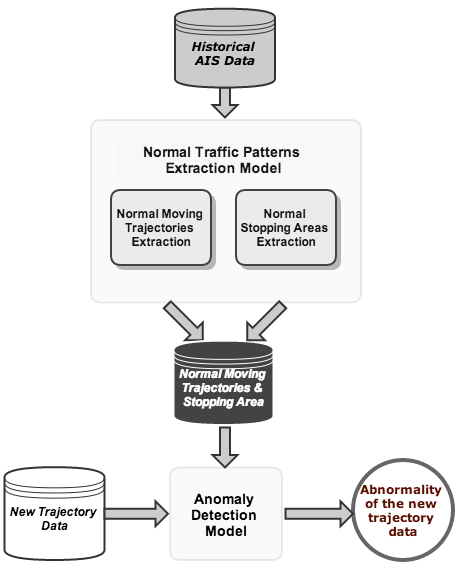
\includegraphics[height=15cm]{structure}
\caption{The framework for Maritime Anomaly Detection. This can be roughly regarded as a two-step procedure. First, the normal traffic extraction model extracts the normal traffic patterns from the historical AIS data repository. Then the extracted Gravity Vectors (GVs) and Sampled Stopping Points (SSPs) are employed by the anomaly detection model to decide the abnormality of the new given trajectory.}
\label{fig:systemStructure}
\end{figure}



%The work for normal traffic patterns extraction is presented in \cite{bigdata2014}.


The proposed clustering-based normal traffic patterns extraction model first divides the AIS data into moving and stopping parts, respectively, based on a stopping SOG (Speed Over Ground) threshold of 0.5 knots. 

For the case where SOG is not less than 0.5 knots, we propose DBSCANSD (Density-Based Spatial Clustering of Applications with Noise considering Speed and Direction) as the basic algorithm to detect the main traffic lanes within the data. DBSCANSD is based on DBSCAN (Density-Based Spatial Clustering of Applications with Noise) \cite{DBScan96} algorithm, modified to consider that for each point of a cluster, the neighborhood of a given radius has to contain at least a minimum number of points with similar SOGs (Speed Over Ground) and COGs (Course Over Ground). The experiments demonstrate that the clusters can reflect normal patterns of the vessels. However, it is not feasible to employ all the points of the clusters to decide the new arriving trajectory data's abnormality. As a result, a representation called Gravity Vector (GV) is proposed. A GV is a vector composed of 5 features: average COG, average SOG, average Latitude, average Longitude and Median Distance. The Median Distance of the GV is the median of the distances between all the trajectory points and the GV in the cell. The Median Distance is to measure the width of navigational lanes. Thus, the output of the moving pattern extraction model can be a set of GVs which carries information about speed, direction, location and even the relative width of the lanes.
%The algorithm's output is a set of Gravity Vectors (GV), which are vectors formed by 5 features: average COG, average SOG, average Latitude, average Longitude and Median Distance.
More details about the process can be found in Section \ref{sec:normal_moving_model}.

%However, in the stopping area extraction model, speed and direction are no longer essential factors for anomaly detection. So the original DBSCAN is first used to extract the stopping clusters. Then similar to the idea of GV, Sampled Stopping Point (SSP) is introduced for data reduction. The process of generating SSPs does not depend on the density of the cluster or the total number of the points in the region, instead, it only depends on the geographic shape of the region. And the experiments show that a small number of SSPs can represent a stopping area well in terms of the shape of the area. 
For the case where the SOG is less than 0.5 knots (stop areas), the original DBSCAN algorithm \cite{DBScan96} is executed because speed (SOG) and direction (COG) are not important factors. Another type of vector is created as output, called Sampled Stopping Point (SSP), which is dependent only on the geographic shape of the region. The experiments show that a small number of SSPs can represent a stopping area well in terms of the shape of the area. More details about the process can be found in Section \ref{sec:normal_stopping_model}.

Once the normal patterns are extracted from the historical AIS data, the second phase is the anomaly detection model (presented in Chapter \ref{ch:anomaly_detection}), can be applied for the new arriving data. In this process, three specialized distances including Absolute Division Distance ($ADD$), Relative Division Distance ($RDD$) and Cosine Division Distance ($CDD$) are proposed to decide the abnormality of one specific data point. Specifically, $ADD$ is employed in the stopping points abnormality detection phase while $RDD$ and $CDD$ are used for the moving part. Furthermore, one anomaly detection algorithm using the three specialized division distances is proposed in Section \ref{sec:anomaly_detection_model}. Although the approach is point-based, which is applicable for real-time AIS surveillance, it is also flexible enough for analysts to set their own threshold for labeling whole trajectories.

%========to add anomaly detection model\cite{toadd}

\section{Scientific Contribution}

This thesis is based on previously published work by the author. The published
work has also been updated and extended with new theoretical and empirical
results in this thesis. The main contributions of this thesis are listed as following:

\begin{quote}
$\bullet$ Proposal of the algorithm of DBSCANSD (Density-Based Spatial Clustering of Applications with Noise considering Speed and Direction), a novel point-based trajectory clustering algorithm which is applicable for various domains.


$\bullet$ Proposal of a normal maritime traffic extraction model based on $stops-and-moves$ approach \cite{stopmove}. 

$\bullet$ Proposal of a normal maritime traffic extraction model associating with the IMO rules. 

$\bullet$ Proposal of two methods to represent the results of clustering, which are the Gravity Vector (GV) for moving clusters and the Sampled Stopping Point (SSP) for stopping clusters.

$\bullet$ Proposal of three specialized division distances measures for maritime anomaly detection.

$\bullet$ Implementation of the proposed maritime anomaly detection framework.

$\bullet$ Evaluation of the proposed maritime anomaly detection framework's effectiveness using both visualization and quantitative approaches.

\end{quote}


\section{Publications}

In this section, the publications published during the author's master study are listed. The first two publications are highly relevant to the thesis while the other two are less relevant to the thesis. Publication 2) first introduces the normal traffic extraction model and has been extended with more detailed explanation in Chapter \ref{ch:normal_traffic_extraction_model}. The anomaly detection model proposed in Chapter \ref{ch:anomaly_detection} is extended from the Publication 1).

\begin{enumerate}[
labelindent=*,
style=multiline,
leftmargin=*,
label= \arabic*)
]

\item Bo Liu, Erico N.de Souza, Casey Hilliard and Stan Matwin, \textbf{Ship Movement Anomaly Detection Using Specialized Distance Measures}, IEEE International Conference on Information Fusion (FUSION 2015), 6-9 July 2015, Washington, DC, USA. (to appear)


\item  Bo Liu, Erico N.de Souza, Stan Matwin and Marcin Sydow, \textbf{Knowledge-based Clustering of Ship Trajectories Using Density-based Approach}, Proceedings of IEEE International Conference on Big Data (IEEE BigData 2014), 27-30 October 2014, Washington, DC, USA. pp. 603-608.

\item  Xiaoguang Wang, Xuan Liu, Bo Liu, Stan Matwin and Erico N.de Souza, \textbf{Vessel Route Anomaly Detection with Hadoop MapReduce}, Proceedings of IEEE International Conference on Big Data (IEEE BigData 2014), 27-30 October 2014, Washington, DC, USA. pp. 25-30.

\item  Robert Warren and Bo Liu, \textbf{Language, Cultural Influences and Intelligence in Historical Gazetteers of the Great War}, Proceedings of IEEE International Conference on Big Data (IEEE BigData 2014), 27-30 October 2014, Washington, DC, USA.  pp. 70-72.


\end{enumerate}




\section{Thesis Outline}

The remainder of the dissertation is organized as follows. %After this introductory chapter, we introduce the background of this thesis in
Chapter \ref{ch:background} presents the related work. It is divided into two parts. %are presented to better illustrate the subject. 
The first part (Section \ref{survey_normal_traffic_extraction}) is about trajectory clustering in general and ship trajectory clustering in the maritime domain in particular.  Section \ref{survey_anomaly_detection} is an overview and survey on anomaly detection techniques used for maritime security.

We present our clustering-based maritime anomaly detection framework in Chapter \ref{ch:normal_traffic_extraction_model} and Chapter \ref{ch:anomaly_detection}. In Chapter \ref{ch:normal_traffic_extraction_model}, we propose our maritime traffic patterns extraction model (Section \ref{sec:normal_moving_model} and Section \ref{sec:normal_stopping_model}) after giving the definition of a trajectory in the maritime domain (Section \ref{sec:trajectory_representation}). As we treat the ship trajectories as two different types based on a speed threshold, moving and stopping, which are explained in more details, Section \ref{sec:normal_moving_model} and Section \ref{sec:normal_stopping_model} propose the normal moving patterns extraction model and normal stopping areas extraction model, respectively. Two different representative  methods, Gravity Vector (GV) and Sampled Stopping Point (SSP) that represent the moving clustering results and stopping clustering results, are introduced accordingly in the two sections. Chapter \ref{ch:anomaly_detection} presents the  anomaly detection model. As our method is a distance-based model, three division distances are first presented in Section \ref{sec:three_division_distances} and then our abnormal detection algorithm is introduced in Section \ref{sec:anomaly_detection_model}.

To evaluate the effectiveness of our framework,  experiments are done in Chapter \ref{ch:evaluation}. First, in Section \ref{sec:exp_1},  to evaluate the normal traffic patterns extraction model, regions of Juan de Fuca Strait and Los Angeles Long Beach are selected and the results are presented in Section \ref{sec:exp_1.1} and Section \ref{sec:exp_1.2}. Then in Section \ref{sec:exp_2}, we conducted another two experiments in the same region of Juan de Fuca Strait. The first one is conducted with the non-labeled data while the second one is done after labelling the data. The results of the first experiment (Section \ref{sec:exp_2.1}) are shown  visually  and  the  second  experiment (Section \ref{sec:exp_2.2}) compares our model's results with the labels by the expert. 

Finally, in Chapter \ref{ch:conclusion} we conclude with a summary and discuss our method's limitations and the potential directions for future work.

\chapter{Related Work}
\label{ch:background}
The problem examined in this thesis can be roughly described as maritime data anomaly detection, a rather specific task. But the increasing demand for detecting and identifying anomalous events from maritime traffic data keeps attracting more and more researchers' attention. 

The approach proposed in this thesis is an unsupervised model based on clustering, so in this chapter, a survey on trajectory clustering and other normal traffic extraction techniques are first given in Section \ref{survey_normal_traffic_extraction}. Since maritime anomaly detection can be considered as a specific type of anomaly detection tasks in maritime domain,  we  survey previous work in anomaly detection in Section \ref{survey_anomaly_detection} and also introduce some representative work done in the maritime domain.


\section{Trajectory Clustering And Maritime Traffic Clustering}
\label{survey_normal_traffic_extraction}

As stated in the previous chapter, our maritime anomaly detection framework is a clustering-based approach, so in this section, we first introduce the problem of trajectory clustering and then provide a survey of various algorithms for solving it. Meanwhile, discussions on the works' limitations for maritime traffic anomaly detection are also conducted while introducing different techniques.

The use of satellites and tracking facilities, such as GPS (Global Positioning System), AIS (Automatic Identification System) and RFID (Radio Frequency Identification Devices) has increased over the past decades, which leads to an increasing number of tracking applications \cite{airspaceMonitoring}. The data spread over various domains and examples include vehicle position data \cite{vehicle_clustering}, airplane tracking data \cite{airspaceMonitoring}, ships or vessels tracking data \cite{CBSMoT}\cite{PallottaFramework}\cite{vespe12}\cite{pallotta13}\cite{DDBscan} and even hurricane or animal movement data \cite{Lee07}\cite{vfkm}.  One crucial task of the applications is trajectory clustering, which is the process to discover the motion patterns from the tracking data.  Exploring different trajectory clustering techniques to extract clusters can help analysts to gain better insights from the data. 

Before investigating different clustering algorithms for trajectories, one point needs to be mentioned. %That is, to extract normal patterns from the tracking data,
Since the goal of trajectory clustering is to find normal paths  by grouping similar trajectories together \cite{Nicolas}, there are lots of works aiming to find proper measures of similarity between trajectories, such as Euclidean distance \cite{vehicle_clustering}, DTW (Dynamic Time Warping) \cite{dtw} and LCSS (Longest Common Subsequence) \cite{lcss}. A comparison between various similarity methods is conducted in \cite{comparison_distances} and majority of these measures are alignment based distances, which are not appropriate for the ship trajectory extraction task due to the sparseness of the AIS data. So in this thesis, we focus more on other clustering-based techniques to address the task.

According to \cite{hanjiaweibook}, clustering is the process of grouping a set of physical or abstract objects into classes of similar objects and the proposed clustering algorithms are usually categorized into four
types: partitioning methods (e.g., K-Means \cite{kmeans} and K-Medoids \cite{kmedoids}), hierarchical methods like BIRCH (Balanced Iterative Reducing and Clustering using Hierarchies) \cite{birch}, density-based methods including DBSCAN \cite{DBScan96}, OPTICS (Ordering Points To Identify the Clustering Structure) \cite{optics} and DENCLUE (DENsity-based
CLUstEring) \cite{denclue}), and grid-based methods such as STING (STatistical INformation Grid-based method) \cite{sting} and CLIQUE (CLustering In QUEst) \cite{clique}).  Among various types of clustering approaches, density-based clustering algorithms can be most suitable for this work because they can find arbitrary shapes of clusters.  In the following paragraph, one representative approach is introduced and the reasons why this type of algorithm is suitable is discussed as well.

 DBSCAN (Density-based spatial clustering of applications with noise) proposed by Martin $et$ $al.$  \cite{DBScan96} in 1996 is one of the fundamental density-based clustering techniques.  The key idea of this clustering algorithm is that for each point of a cluster the neighborhood of a given radius has to contain at least a minimum number of points. So the algorithm requires two additional parameters, $eps$ and $minPts$, as input, where the $eps$ is the radius and $minPts$ is the minimum number of points required to form a dense region.  After applying DBSCAN on a set of points, the points are classified as core points, border points and noise points. Here both core points and border points form clusters while the noise points are filtered out. Compared to other types of clustering algorithm, DBSCAN has two main advantages which make it well-suited for the maritime trajectory clustering task. Firstly, the algorithm can provide good results in many cases since it is able to discover clusters of arbitrary shapes and it is robust to detect outliers \cite{hanjiaweibook}.  Secondly, unlike K-Means \cite{kmeans}, users are not required to provide the number of expected clusters before running the algorithm.  However, one crucial limitation is that the original DBSCAN algorithm can only take into account location data (Longitude and Latitude), which cannot satisfy the requirement of performing this anomaly detection in the maritime domain.  Therefore, as part of our work, we extend DBSCAN to adopt other attributes, such as speed and direction, to find normal traffic patterns from the moving trajectory dataset.


To handle specific issues of tracking data, researchers propose various approaches which extend the original DBSCAN in different ways.   One method called DB-SMoT (Direction Based Stops and Moves of Trajectories) \cite{DDBscan} is a clustering method based on the direction change in a minimal amount of time. For example, if there is a sequence of points with enough direction variance but the duration between the last point and the first point is less than the minimal time threshold, the sequence will not be considered as a final cluster. The main purpose of the algorithm is to find interesting places using single fishing ship trajectory data. The methodology introduced by the authors is simply using DBSCAN to cluster all the data points with a bigger direction variation than the pre-defined threshold. This algorithm is helpful in this specific scenario but cannot be fit for anomaly detection in consideration of the significance of the speed. Different from DB-SMoT, another work done by Palma $et$ $al.$ \cite{CBSMoT} called CB-SMoT (Clustering-Based Stops and Moves of Trajectories) takes speed into account. However, due to the goal of the paper which is also to find interesting places, the method only uses speed as a threshold and then conducts clustering work on the low-speed data set. In this case, the idea of CB-SMoT can be adopted for extracting stopping areas from AIS data. In Section \ref{sec:normal_stopping_model}, we present our approach to cluster and represent the stopping areas in the sea. However, CB-SMoT cannot be applied to extract different clusters with various normal speeds from navigational data set. 



One partition-and-group framework, TRACLUS (TRAjectory CLUStering) \cite{Lee07}, also uses density-based clustering to detect general lanes. TRACLUS is proposed by Lee $et$ $al$. \cite{Lee07} and is one of the main references in the field of trajectory clustering.  The algorithm is trajectory-based. It tries to solve the clustering problem from the view of line segments of given whole trajectories. The general procedure of TRACLUS is to first partition each trajectory into line segments and then group close line segments into one particular cluster.  The reason why they partition the whole track into short sub-segments before the clustering process is that clustering trajectories as a whole could lose similar portions of the trajectories \cite{Lee07}. Lastly, a representative trajectory is computed for each cluster. One limitation of this strategy is that it cannot consider the speed, which is very important to maritime traffic tasks. Another problem in the adaptation of this algorithm to our task is that TRACLUS is sensitive to the parameters ($eps$ and $MinLns$). Although the paper provides an optimal estimation algorithm for thresholds, the experiments conducted in \cite{Lee07} demonstrate that the generated pair of parameters are not guaranteed to be optimal. When we tried to employ the algorithm for extracting normal ship trajectories, a satisfactory result could not be obtained even after a large number of trials. Fortunately, compared to TRACLUS, our model is less sensitive to the parameters as long as the analysts have some knowledge of the maritime domain.


One popular scenario of applying trajectory clustering techniques is video surveillance and monitoring systems. After distinguishing the foreground objects from the background  \cite{videosurveillance3} and identifying
the positions of the moving objects (e.g. cars, pedestrians, etc.) in the foreground image, trajectory clustering approaches can be applied to group similar trajectories of the moving objects.  In the work done by Paciarelli $et$ $al$.  \cite{videosurveillance1}\cite{videosurveillance2}, a dynamic model is presented to group similar trajectories into clusters. The model is essentially maintaining a forest of trees to represent the normal patterns. The prefix of one particular node, from the root node to the current node, stands for a specific normal path formed by all the clusters in the branch (including the root and the node itself). When a new trajectory is fed into the system, a prefix matching will be conducted and the best matching cluster will adopt the new arriving trajectory to update its properties, including physical coordinates and variances of the trajectory points inside the cluster. One issue of the approach is that a large number of trees need to be stored, because different trajectories may have different starting points and each start point needs a corresponding root node. Another limitation is that the prefix matching phase requires complete trajectories to be observed, which is infeasible in maritime traffic tracking. It is common to have gaps in the AIS data stream and the gaps can vary from milliseconds to days. In addition to the above two problems, similar to TRACLUS \cite{Lee07}, it cannot take speed into account, which is a fundamental issue in coastal surveillance. Currently in this thesis, the point-based approach is proposed to address the issue of the inconsistently updated trajectory data and no concern about prefix matching exists.

Inspired by the work done by Paciarelli $et$ $al$.  \cite{videosurveillance1}\cite{videosurveillance2}, Guillarme $et$ $al$. propose a trajectory-based ``unsupervised normalcy model'' \cite{Nicolas} for  S-AIS data. This work is also based on stop and move framework \cite{stopmove} and applies corresponding strategies on moving trajectories and stopping areas. Similar to TRACLUS \cite{Lee07}, this technique is also a partition-and-group framework, which first partitions the historical trajectories into sub-segments. To extract normal patterns from moving trajectories, the authors introduce a technique based on the OPTICS algorithm \cite{optics}. OPTICS has the advantage of handling situations where clusters exist at different density levels, but it needs more experts' input knowledge for selecting relevant clusters from different clusters levels, which is more complicated than our non-hierarchical clustering approach.  So this is less feasible for applying the algorithm in a large area with complicated traffic routes. Then for stopping areas extraction, the authors present a representation to estimate the locations and the spatial extent of a stopping area. This method is similar to their solution used for moving trajectories, that is, it tries to use one particular node to represent an arbitrary shape of region. This will cause a bias while it comes to coastal stopping areas since the areas might not be in circle shapes. Fortunately, the Sampled Stopping Points proposed in this work can represent arbitrary shapes of regions well.


Ferreira $et$ $al$. \cite{vfkm} propose a strategy called VFKM (Vector Field K-Means) based on vector field fitting. The idea behind their method is to induce a similarity notion on the data set by using streamlines of a single vector field. Two main elements of this algorithm are fitting the vector fields and assignment of trajectories to clusters \cite{vfkm}. Since the approach assigns the trajectories to the vector fields, it is also a trajectory-based method. VFKM is an iterative model similar to original K-Means \cite{kmeans} and two main steps are involved in each iteration. First, the trajectories are partitioned randomly into K clusters (similar to the initialization of original K-Means). Then the clusters are updated by assigning each trajectory to the vector field that it fits best. These two steps are repeated iteratively until a convergence criterion is met. There are several limitation related to the algorithm. Firstly, as mentioned by the authors \cite{vfkm}, the performance of the algorithm is sensitive to the choice of initial clusters. Secondly, although this method can consider other features (e.g. direction and speed) of the trajectory data, it cannot provide a representative trajectory. Instead, the algorithm output is $k$ representative vector fields which cannot be employed in our case. Fortunately, in our thesis, the output of the maritime traffic extraction model is two sets of representative vectors (Gravity Vectors and Sampled Stopping Points), which is feasible for handling the anomaly detection problem.




One work which provides mechanisms to manage traffic in the ocean that is similar to ours is an unsupervised framework called TREAD (Traffic Route Extraction and Anomaly Detection), proposed by Pallotta $et$ $al$. \cite{PallottaFramework}\cite{vespe12}\cite{pallotta13}. It is designed to detect low likelihood behaviors and predict future vessel positions from maritime traffic data. TREAD is a point-based framework and the traffic routes are built by the way-points generated by the clustering process, that is, the route objects are directly formed by the flow vectors of the vessels whose paths connect the derived way-points. The assumption of using waypoints to build the traffic lanes is that the vessels' trajectories are composed of a set of connected straight lines. Another similar methodology proposed by Gariel $et$ $al$. \cite{airspaceMonitoring} is also a way-point-based clustering framework for handling airspace monitoring. The objective of the method is to identify and group the turning points into way-points and to use the sequence of way-points to represent the aircraft's trajectories. To get the way-points from the historical flight data, two traditional clustering algorithms are employed. When the spatial distribution is sparse, K-MEANS \cite{kmeans} is used, and when the distribution is dense, DBSCAN \cite{DBScan96} is used. This point-based idea has a practical advantage of handling trajectories of unequal length or with gaps, which is common due to the low satellite coverage of AIS around the world. The main difference in relation to TREAD \cite{PallottaFramework} relies on the fact that our work tries to directly map the  rules defined by IMO into real data available from AIS readings.


Another main advantage of the clustering framework proposed in this thesis is that in the clustering process the IMO rules, particular Traffic Separation Schemes, are taken into account, which is not the case in previous works. Therefore, our approach maps rules defined by IMO directly to the AIS data, and in that sense it is similar to the Candide \cite{Candide} system, which is a digital face reconstruction mask. Candide uses a pre-defined digital face mask to be adjusted in a facial picture, and allows the generation of new facial  expressions  without any extra information.  From the rule mapping perspective, this work does the same, with the difference that we use the set of rules defined by IMO and check if vessels are following them.






\section{Anomaly Detection in Maritime Surveillance}
\label{survey_anomaly_detection}

The objective of anomaly detection is to find patterns in data that do not conform to expected behavior and these nonconforming patterns are often referred to as anomalies or outliers \cite{chandola}. Anomalies or outliers are related to, but distinct from, noise in the data. As defined in \cite{chandola}, noise is some patterns or phenomenons in data that are not of interest to the analyst, but act as a hindrance to data analysis. Thus, activities on handling these unwanted noise involve noise removal \cite{teng1990adaptive} and noise accommodation \cite{rousseeuw2005}. But in anomaly detection tasks, the outliers or the anomalies are the patterns which attract much attention from the analysts in various domains, such as fraud detection for credit cards \cite{creditcard}, insurance \cite{insurance}, or health care \cite{healthcare}, intrusion detection
for cyber-security \cite{cyber} and military surveillance for enemy activities \cite{chandola}.  In this thesis, our work focuses on detecting the anomaly navigational behaviors  of the ships or vessels. 

Maritime Anomaly Detection techniques primarily fall into two categories: statistical modelling \cite{gmm}\cite{kde}\cite{Gerben} and predictive modelling \cite{PallottaFramework}\cite{bn_White}\cite{bn_Richard}. The general idea of  statistical techniques for anomaly detection is to fit a statistical model for normal behaviors with the given data set and then apply a statistical inference test to determine if a previously unseen instance belongs to the model \cite{chandola}. Approaches based on predictive models usually predict future status information (e.g. position, speed and course) of a particular vessel and then compare the real data with the prediction to decide the abnormality. Additionally, there is another type of approach trying to solve the problem based on predefined rules. One representative work was done by Roy $et$ $al$. \cite{roy2010rule}\cite{roy2009categorization} and an expert system for automated anomaly detection was introduced.  As we know, one limitation about these kind of systems is that they are  relying on the knowledge of predefined rules, as a result, much effort needs to be done to categorize anomalies. In the papers \cite{roy2010rule}\cite{roy2009categorization}, the authors identified a taxonomy of kinematic and geo-spatial concepts in the vessels tracking domain and the taxonomy has to be updated once a new rule is found.  Since not much work focuses on rule-based type of techniques, this survey of maritime anomaly detection is more about the other two main categories.

In the maritime domain, the majority of statistical models are built upon the momentary kinematic features (position, course, speed and acceleration rate) of individual vessels. 

Laxhammar \cite{gmm} used a Gaussian Mixture Model (GMM)  and a greedy version of Expectation-Maximization (EM)\nomenclature{EM}{Expectation Maximization} for clustering. A GMM can be regarded as an ensemble model of $K$ multivariate Gaussian distributions (mixture components). GMM is an extension of single Gaussian and it has the advantage of approximating arbitrarily complex distributions in arbitrarily high dimensions.  The greedy EM-learning (greedy Expectation-Maximization-learning) algorithm, an extension to the classical EM-algorithm,  is employed to determine the optimal number of components (or distributions) and the parameter set for all the distributions. So the greedy EM algorithm is basically an iterative model with mainly two steps in each iteration; the first step is to insert a new component and the second step is to apply classical EM until convergence.  Then in order to label new data, the likelihood of the new point will be first calculated based on the probability distribution obtained from the clustering phase. Further, it will be classified as abnormal if the likelihood is below a certain predefined alarm threshold.

According to \cite{comparison}, GMM is not an optimal model because it needs an assumption that the distribution of vessel positions along the major axis of the sea lane segments is uniform.  To tackle this issue, in \cite{kde}, the authors propose to use adaptive Kernel Density Estimator (KDE) for estimating unknown probability densities and modelling arbitrary sea lanes.  KDE, also known as the Parzen Window method, is a non-parametric model and the estimated PDF (Probability Density Function) can be determined based merely on the training data, which is superior to GMM. Then in the anomaly detection phase, the anomaly detector is sequentially applied to the incoming data. The value of new incoming point's density is calculated under the null hypothesis (no anomaly) and this value is then compared with a detector parameter related to false alarms for deciding the new point's abnormality.

%first assume that the normal patterns have been extracted from the data mining stage using historical trajectory data and then conduct the statistical analysis on the new incoming AIS data in the framework of adaptive Kernel Density Estimator (KDE).

A comparison between the two approaches above \cite{gmm} and \cite{kde} is given in \cite{comparison}, demonstrating that the anomaly detection results from both models are not satisfactory %as the expected trajectory distance observed before detection is considered rather long.  
as the two models detect the anomalous segments after rather long distances (three kilometers and four kilometers respectively) while an expected effective anomaly detector should detect such behaviors at a shorter distance \cite{comparison}. %an earlier stage. \cite{comparison}
Another disadvantage of the two statistical methods is that it is hard to interpret in terms of anomaly types, even if they could find anomaly patterns promptly. Once a point is determined to be abnormal, the likelihood value in \cite{gmm} and the density value in \cite{kde} cannot indicate the types of the abnormality. For example, the analysts cannot know whether the point deviates too far away from the normal lanes or the vessel sails too slow or too fast compared to normal speed.




In \cite{Gerben}, Gerben $et$ $al.$ propose a technique based on Machine Learning models. In their work, different trajectory alignment kernels (Dynamic Time Warping \cite{dtw} and Edit Distance \cite{edit_distance}) are applied with one-class SVMs (Support Vector Machine) \cite{svm} for detecting the outlying trajectories. This trajectory-based method requires that the complete trajectory has been observed before it can be classified as normal or anomalous \cite{phdthesis}, which is not applicable for sequential anomaly detection in incomplete trajectories (real-time AIS surveillance), unlike our proposed point-based method.



Pallotta $et$ $al.$ \cite{PallottaFramework} suggest the use of rule-based and low-likelihood models for anomaly detection. As stated in a previous paragraph, the rule-based techniques generate alerts based on a set of pre-defined rules. So the rules defined in this approach are similar to those in other knowledge-based work, which require maritime domain experts' knowledge. As an example,  no specific rules defined for maximum speed in different sea regions can be found in IMO publications \cite{tss}\cite{anabook}, so the maximum speed pre-defined in a port area can only be accurately estimated by a specialist knowledgeable about the area. Similar to the work done in \cite{gmm}, the low-likelihood anomaly detection aims at detecting deviations from the normal patterns or distributions derived from the training AIS data. For this low-likelihood detection, a Weibull model was employed (a parametric exponential-like model), along with a sliding time window technique to avoid problems with incomplete and intermittent tracks.



Similar to the work done in \cite{PallottaFramework}, Nevell \cite{bn_White} proposes to use a Bayesian approach to predict the future route of a particular vessel for comparison. This methodology is based on a node-sparse network, built from different kinds of coastal nodes. The idea of pre-defining a global maritime traffic network is also adopted in \cite{Soleimani} where the network is constructed based on the historical data. But instead of a Bayesian approach, Soleimani $et$ $al.$ \cite{Soleimani} employ the $A*$ \cite{astar} algorithm to decide the optimal or expected route.
In \cite{bn_Richard}, the authors insist that an overall threat is indicated by a sequence of the individual behaviours. Therefore, five specific anomalies (deviation from standard route, unexpected AIS activity, unexpected port arrival, close approach with another ship and entering a zone known as illegal exchanges) are introduced to extend Nevell's work \cite{bn_White} to assess the probability of a higher-level threat based on a constructed Bayesian Network.
%An idea of using Bayesian Network to extend the David Nevell's work \cite{bn_White} is given in \cite{bn_Richard}, where five specific anomalies is introduced: deviation from standard route, unexpected AIS activity, unexpected port arrival, close approach with another ship and entering a zone known as illegal exchanges. The authors insist that an overall threat is indicated by a sequence of the individual behaviours and they assess the probability of a higher-level threat based on Bayesian Network. Therefore, the process can be regarded  fusion by combining  the individual detectors' outputs to give a single number between zero and one \cite{bn_Richard}. 

One issue with the work described in \cite{bn_White}\cite{bn_Richard} is that it cannot incorporate speed into deciding if a trajectory is anomalous; instead the judgement is based only on position. Another problem is that a pre-defined network may not be applicable in many near-port regions due to the nature of port traffic. Traffic in near-port areas is usually  variable and the vessels are not always following straight lanes (optimal routes in \cite{bn_White}\cite{bn_Richard}). Fortunately, both of these problems are handled with our approach.

%And as our approach is based on the clustering process

%The clusters are arbitrary shapes of traffic lanes, which can reflect the complicated traffic in any areas

The anomaly detection model in this thesis uses the results of the clustering framework presented in Chapter \ref{ch:normal_traffic_extraction_model}, which generates normal moving patterns and arbitrary shapes of stopping areas.
%, and generates an anomaly ratio.
%that can be used as a threshold to identify anomalous points in a track. 
The proposed anomaly detection method is point based but is capable of handling trajectory tracks. For each track the algorithm will return an anomaly ratio. The ratio is based on three types of specialized distances to take position, direction and speed into consideration.




%chapter 2 Normal Pattern Extraction
\chapter{Normal Traffic Patterns Extraction Model}
\label{ch:normal_traffic_extraction_model}

Vessels consistently follow different movement patterns in different areas. For instance, cargo ships may travel along straight lines at high speed in the middle of the sea, while they may frequently adjust their directions at low speed in the port or offshore platform areas. 

As a consequence, Spaccapietra \cite{stopmove} introduced a model to reason about trajectories, which is called stops and moves. So a trajectory can be treated as a sequence of moves and stops \cite{stopmove}, and in the work done by \cite{vespe12}\cite{PallottaFramework}\cite{Nicolas}, maritime trajectories analysis is conducted from these two different aspects as well, moving patterns and stopping patterns distinguished by a speed threshold. According to \cite{Nicolas}, the stop and move model has two main advantages: 1) stopping areas are interesting areas which need to be discovered; 2) stopping points are one important source of noise during trajectory clustering and stopping points do not include any motion information for path modelling. In addition to the above mentioned advantages, another benefit is that it can help to decrease the search space complexity during moving trajectories clustering since the stopping points are filtered out before applying the algorithm. %and as as result, it helps to enhance the moving trajectories' clustering performance.  

In this work, we employ a similar method to extract different normal patterns from the historical AIS dataset with a stopping SOG (Speed Over Ground) threshold of 0.5 knots. More specifically, we first divide the historical AIS data into two subsets: the set of moving points (with SOG not less than 0.5 knots) and the set of stopping points (with SOG less than 0.5 knots). Instead of merely clustering the waypoints of the trajectory data \cite{vespe12}\cite{PallottaFramework}, normal moving trajectories and arbitrary shapes of stopping regions will be extracted based on the entire moving and stopping dataset in the specific area, respectively.

In this chapter, a definition for a trajectory in the maritime domain (Section \ref{sec:trajectory_representation}) is first given and then the model for extracting normal patterns from the historical AIS data is proposed.  %This clustering-based normal traffic patterns extraction model first divides the AIS data into moving and stopping parts respectively based on a stopping SOG (Speed Over Ground) threshold of 0.5 knots. 
For the case where SOG is not less than 0.5 knots (moving patterns), we propose DBSCANSD (Density-Based Spatial Clustering of Applications with Noise considering Speed and Direction) as the basic algorithm to detect the main traffic lanes within the data. The algorithm's output is a set of Gravity Vectors (GV), which are vectors formed by 5 features: average COG, average SOG, average Latitude, average Longitude and Median Distance. In Section \ref{sec:normal_moving_model},  for the case where the SOG is less than 0.5 knots (stopping areas), the original DBSCAN \cite{DBScan96} algorithm is executed because speed and direction are not important factors. Another type of vector is created as output, labelled Sampled Stopping Point (SSP), which is dependent only on the geographic shape of the region. (Section \ref{sec:normal_stopping_model}) 

\section{Representing Trajectory Data} \label{sec:trajectory_representation}

\begin{definition}
\label{def:trajectory_raw}
(Trajectory) A trajectory is a finite sequence T = (($x_1, t_1$), ($x_2, t_2$), ... , ($x_m, t_m$)). Each data point $x_i$ corresponds to a multi-dimensional feature vector of a moving object at time point $t_i$, where $t_i < t_{i+1}$ for i =1,..., m-1.
\end{definition}

A trajectory can be defined as a data type representing the movement of an object. A trajectory can be represented by a multidimensional time series \cite{aggarwal2013data} or a sequence of multi-dimensional points \cite{Lee07}. In this thesis, we modify the definition of its raw form (Definition \ref{def:trajectory_raw}) \cite{phdthesis} to adapt it for our work. The new definition of a ship trajectory is as following:

\begin{definition}
\label{def:trajectory}
(Trajectory in Maritime Domain) A trajectory is a finite sequence T = (($x_1, t_1$), ($x_2, t_2$), ... , ($x_m, t_m$)) where $x_i$ is a set of $<Latitude, Longitude, COG, SOG>$ and $t_i$ is the time-stamp.
\end{definition}

Here in Definition \ref{def:trajectory}, each vector $x_i$ is called a \textbf{trajectory point}, but in this thesis, we simply use \textbf{point} or \textbf{data point} where the context is clear.


\section{Normal Moving Trajectories Extraction}
\label{sec:normal_moving_model}


As stated at the beginning of the chapter, given a data set of AIS historical tracking points, we divide them into stopping and moving parts based on the threshold of 0.5 knots. In this section, we present our moving trajectory extraction model.

As we know, compared to stopping patterns, the moving part plays a more important role in the anomaly detection task since there is a higher collision risk for a vessel sailing at high speed than at low speed in the stopping areas. To extract normal patterns from the moving AIS data, we first propose the new clustering algorithm DBSCANSD (Density-Based Spatial Clustering of Applications with Noise considering Speed and Direction).

\subsection{Density-Based Spatial Clustering of Applications with Noise considering Speed and Direction}


Density-Based Spatial Clustering of Applications with Noise considering Speed and Direction (DBSCANSD), shown in Algorithm \ref{algo1}, is a density-based clustering algorithm based on the algorithm DBSCAN \cite{DBScan96}. The main observation behind our approach is that it is common for different types of ships to sail with different velocities in one similar area of the sea. For instance, the cruise speed of a cargo ship can be faster than a fishing ship. Even the same type of vessels can behave differently in relation to direction. Imagine that an oil tanker sails between two different countries. When the vessel is full, its speed is slower than when it is empty. 

\begin{definition}
\label{def:epsneighborhood_old}
(Eps-neighborhood of a point) Given a databse D of moving trajectory points in a specific area, the $Eps-neighborhood$ of a point p, denoted by $N_{\epsilon}(p)$, is defined by $N_{\epsilon}(p)$ = $\{ q\in D \mid dist(p, q) < \epsilon$\}
\end{definition}

\nomenclature{$N_{\epsilon}(p)$}{Eps-neighborhood of a point $p$}

As discussed in Chapter \ref{ch:background}, the key idea of DBSCAN \cite{DBScan96} is that for each point of a cluster the neighborhood of a given radius has to contain at least a minimum number of points. Here in this thesis, we adopt this idea but also consider two other factors, maximum speed variance ($MaxSpd$) and maximum direction variance ($MaxDir$). The intuition behind this is that the neighbors of a trajectory point should be not only near enough, but also with similar COG (Course Over Ground) and SOG (Speed Over Ground). Thus, we can modify the definition of Eps-neighborhood (Definition \ref{def:epsneighborhood_old}) in \cite{DBScan96} to Definition \ref{def:epsneighborhood_new}.


\begin{definition}
\label{def:epsneighborhood_new}
(Eps-neighborhood of a trajectory point)
Given a database $D$ of moving trajectory points in a specific area, the $Eps-neighborhood$ of a trajectory point p, denoted by $N_{\epsilon}(p)$, is defined by $N_{\epsilon}(p)$ = $\{ q\in D \mid dist(p, q) < \epsilon$ and $\left|p.SOG-q.SOG\right|<MaxSpd$ and $\left|p.COG-q.COG\right|<MaxDir$\}
\end{definition}


Note that $dist(p,q)$ is the Geographical Distance \cite{gpsDistance} between $p$ and $q$, instead of Euclidean distance, because it is necessary to take in consideration the Earth's curvature to calculate distances.

Then in the following, we also give the formal definitions of other essential notions for our density-based algorithm. The definitions are changed from the ones originally defined for 2-Dimensional points in the algorithm of DBSCAN \cite{DBScan96} to those for trajectory points.

\begin{definition}
\label{def:core_trajectory_point}
(Core trajectory point)
Given a database $D$ of moving trajectory points in a specific area, a trajectory point p in $D$ is called a core trajectory point w.r.t. the parameters of $\epsilon$, MinPts, MaxSpd and MaxDir if $\left|N_{\epsilon}(p)\right| \geq MinPts$ \}
\end{definition}

\begin{definition}
\label{def:directly_density_reachable}
(Directly density-reachable)
Given a database $D$ of moving trajectory points in a specific area, a trajectory point p in $D$ is directly density-reachable from another trajectory point q in $D$ w.r.t. the parameters of $\epsilon$, MinPts, MaxSpd and MaxDir if $p \in N_{\epsilon}(q) $ and $\left|N_{\epsilon}(q)\right| \geq MinPts$ \}
\end{definition}

From Definition \ref{def:directly_density_reachable}, we can find out whether point $q$ is a core trajectory point according to Definition \ref{def:core_trajectory_point}. Because $\left|N_{\epsilon}(q)\right| \geq MinPts$, $q$ is a core trajectory point. If the point $q$ is also directly density-reachable from the point $p$, the point $q$ will be also a core trajectory point clearly. But when the point $p$ is not a core point and it is directly density-reachable from core point $q$, the point $p$ is called \textbf{Border Trajectory Point}.

\begin{definition}
\label{def:density_reachable}
(Density-reachable)
Given a database $D$ of moving trajectory points in a specific area, a trajectory point p in $D$ is density-reachable from another trajectory point q in $D$ w.r.t. the parameters of $\epsilon$, MinPts, MaxSpd and MaxDir if there is a chain of trajectory points $p_1,..., p_n, p_1 = q, p_n = p$ such that $p_{i+1}$ is directly density-reachable from $p_i$  ( 1 $\leq$ $i<n$) \}
\end{definition}

From Definition \ref{def:density_reachable}, we can find the trajectory point $p$ can be either a border trajectory point or core trajectory point if $p$ is density-reachable from point $q$. But the point $q$ and other points (except $p$) in the chain must be core trajectory points. Therefore, this relation is transitive, but it is not symmetric \cite{DBScan96}.


\begin{definition}
\label{def:density_connected}
(Density-connected)
Given a database $D$ of moving trajectory points in a specific area, a trajectory point p in $D$ is density-connected to another trajectory point q in $D$ w.r.t. the parameters of $\epsilon$, MinPts, MaxSpd and MaxDir if there is a trajectory point o such that both p and q is density-reachable from o w.r.t.  $\epsilon$, MinPts, MaxSpd and MaxDir\}
\end{definition}

However, if there exist multiple trajectory points ($p_1$, ..., $p_n$ ) that are density-reachable from one core trajectory point $o$, then points $p_1$, ..., $p_n$ can be all border trajectory points.  In such a cluster, one border trajectory point ($p_1$) is obviously not density-reachable from any other border points ($p_2$, ..., $p_n$). So it is necessary to define a relationship (Definition \ref{def:density_connected}) for any pairs of two border trajectory points in the same cluster.

\begin{figure}[!htb]
\centering
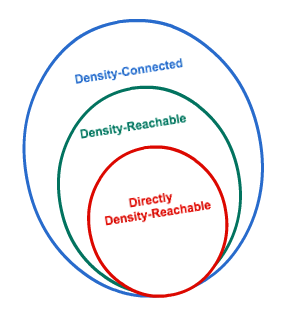
\includegraphics[width=3in]{relations.png}%height=8cm
\caption{Three defined relations for the density-based clustering algorithm.}
\label{fig:relations}
\end{figure}


With the three density-based relations defined as above, it is easy to see the relationships between them. Figure \ref{fig:relations} demonstrates these relationships. For example, if there are two trajectory points $p$ and $q$, and $p$ is directly density-reachable from $q$, $p$ will be not only density-reachable but also density-connected from $q$. However, if $p$ is density-reachable from $q$, it will be also density-connected from $q$ but may be not directly density-reachable from $q$. 


%%%%definition for cluster
Now the concepts of \textbf{Cluster} and \textbf{Noise} (Definition \ref{def:cluster} and Definition \ref{def:noise} respectively) can be defined based on the above three relations (Directly density-reachable, Density-reachable and Density-connected):

\begin{definition}
\label{def:cluster}
(cluster)
Given a database $D$ of moving trajectory points in a specific area, a cluster C w.r.t. $\epsilon$ and MinPts is a non-empty subset of D satisfying the following two conditions:

1) $\exists$ p $\in$ C, $\forall$ q $\in$ D, if q is density-reachable from p w.r.t. the parameters of $\epsilon$, MinPts, MaxSpd and MaxDir, then q $\in$ C

2) $\exists$ p $\in$ C, $\forall$ q $\in$ D, if p is density-connected to q w.r.t. the parameters of $\epsilon$, MinPts, MaxSpd and MaxDir, then q $\in$ C
\}
\end{definition}


\begin{definition}
\label{def:noise}
(noise)
Given a database $D$ of moving trajectory points in a specific area, and $C_1$, ..., $C_k$ are the clusters of D w.r.t. the parameters of $\epsilon$, MinPts, MaxSpd and MaxDir, i = 1, ..., k, then the noise is the set of trajectory points in the database D not belonging to any cluster $C_i$, i.e. noise = $\{$ p $\in$ D $\mid$ $\forall$ i: p $\notin$ $C_i$ $\}$
\}
\end{definition}


%\floatname{algorithm}{Procedure}
\renewcommand{\algorithmicrequire}{\textbf{Input:}}
\renewcommand{\algorithmicensure}{\textbf{Output:}}


\begin{algorithm}
\caption{DBSCANSD}\label{algo1}
\begin{algorithmic}[1]
\Procedure{DBSCANSD}{$DatasetM$, $eps$, $MinPts$, $MaxDir$, $MaxSpd$}
\State  Mark all points in moving dataset $DatasetM$ as unclassified
\State $clusterList \gets$ empty list
\For {each unclassified point $P$ in $DatasetM$}
    \State Mark $P$ as classified
    \State $neighborPts \gets$ queryNeighborPoints ($DatasetM$, $P$, $eps$, $MinPts$, $MaxDir$, $MaxSpd$)
    \If {$neighborPts$ is not $NULL$} 
        \State  $clusterList$.add($neighborPts$)
    \EndIf
\EndFor
\For {each cluster $C$ in $clusterList$}
    \For {each cluster $C'$ in $clusterList$}
        \If {$C$ and $C'$ are different clusters}                     \If{mergeClusters($C$, $C'$) is TRUE}
                \State $clusterList$.remove($C'$)
            \EndIf
        \EndIf
    \EndFor
\EndFor
\State \textbf{return} $clusterList$
\EndProcedure

\Procedure{queryNeighborPoints}{$data$, $P$, $eps$, $MinPts$, $MaxDir$, $MaxSpd$}
\State $cluster \gets$ empty list 
\For {each point $Q$ in data}
    \If {distance($P$,$Q$) $<$ $eps$} 
        \If {$\left|P.SOG-Q.SOG\right|< MaxSpd$}
            \If {$\left|P.COG-Q.COG\right| < MaxDir$}
                \State $cluster$.add($Q$)
            \EndIf
        \EndIf
    \EndIf
\EndFor
\If {$cluster$.size $>$ $MinPts$}
    \State Mark $P$ as core point
    \State \textbf{return} $cluster$
\EndIf
\State \textbf{return} $NULL$
\EndProcedure
\algstore{dbscansd}

\end{algorithmic}
\end{algorithm}

\begin{algorithm}
\begin{algorithmic}[1]
\algrestore{dbscansd}

\Procedure{mergeClusters}{$clusterA$, $clusterB$}
\State $merge \gets FALSE$
%\If {$clusterA$ or $clusterB$ is empty}
%    \State \textbf{return} $FALSE$
%\EndIf
\For {each point $Q$ in $clusterB$}
    \If {point $Q$ is core point and $clusterA$ contains $Q$}
        \State $merge \gets TRUE$
        \For {each point $Q'$ in $clusterB$}
            \State $clusterA$.add($Q'$)
        \EndFor
    \State break
    \EndIf
\EndFor
\State \textbf{return} $merge$
\EndProcedure


\end{algorithmic}
\end{algorithm}





Algorithm \ref{algo1} presents the procedures of DBSCANSD. It requires 5 parameters ($DatasetM$, $eps$, $MinPts$, $MaxDir$, $MaxSpd$) as input. $DatasetM$ is a list of all the moving points in the trajectories.  $eps$ and $MinPts$ are the reachable distance and reachable minimum number of points (see Ester $et$ $al$ \cite{DBScan96}).  The other two, $MaxDir$ and $MaxSpd$, are the two new parameters (maximum direction variance and maximum speed variance).  The algorithm starts with a random selected trajectory point and then retrieves all its neighbour points. If its neighbour points' number is exceeding the threshold of $MinPts$, the point is marked as a core trajectory point and all its neighbours are adopted in the cluster. This procedure then iterates until all the points have been visited and the output is a set of clusters. \\



\noindent\textbf{Time Complexity Analysis of DBSCANSD algorithm:}

\noindent\texttt{procedure QueryNeighbourPoints} (lines 15-25):

\noindent The dominating operation is the \texttt{if} test (lines 18-20), data size: $n=$\texttt{data.size}.
The implementation presented in Algorithm \ref{algo1} has linear time complexity $O(n)$ where n is the size of the \texttt{data} set. However, if some spatial index is used the time complexity can be reduced to $O(log(n))$.


\noindent\texttt{procedure MergeClusters} (lines 26-34):

\noindent The dominating operation is the \texttt{contains} test operation (line 29), the data size is the number of elements the second cluster $b=$\texttt{clusterB.size}.
In the simple implementation presented in Algorithm \ref{algo1} the worst time complexity is linear $O(b)$, if we assume the constant time cost of \texttt{contains} operation (this can be achieved by keeping a hash-set structure). However, this procedure can be accelerated with more sophisticated data structures, in particular avoiding adding elements one by one.

\noindent\texttt{procedure DBSCANSD} (lines 1-14):

\noindent Finally, the main procedure \texttt{DBSCANSD} is dominated by the two consecutive loops: point neighbourhoods computation (lines 4-8) and cluster merging (lines 9-13). The data size is the total number of elements $n=$\texttt{DataSetM.size}. The initialisation (line 3) is linear $O(n)$. Each of the two loops (lines 4-8 and lines 9-13) in the simple implementation presented in Algorithm \ref{algo1} can be bounded with the quadratic time complexity $O(n^2)$, however, as we mentioned above, it is possible to accelerate it by applying more sophisticated data structures in the sub-procedures. To sum up, the \texttt{DBSCANSD} algorithm has at most quadratic time complexity $O(n^2)$ but there is definitely a room for improvement that will be further explored as the part of the future work. \\



We use external knowledge based on the Traffic Separation Schemes (TSS) \cite{tss} defined by IMO to adjust the parameters of the algorithm; therefore, we are using the lanes defined in IMO publications to fit the clustering results. As we know, once the area is determined, the two parameters $MaxDir$ and $MaxSpd$ should be fixed. During this thesis work, multiple pairs of values were tested to find the optimal $MaxDir$ and $MaxSpd$. Our experiments indicate that 5$^{\circ}$ and 5 knot are the best parameters for both tested ports (Los Angeles Long Beach area and Juan De Fuca Strait area). 

On the other hand, the parameters $eps$ and $MinPts$ must be defined for each port. Thus, another set of experiments were done to select the best pair for each area. For instance, when a lane generated by the clustering algorithm has any gaps compared to the one in the IMO TSS regulations, the analyst must increase the value of $eps$ or decrease that of $MinPts$. In this way, the lanes with lower densities might be adopted as parts of the clusters to fill in the gaps. The two parameters $eps$ and $MinPts$ selected in this procedure will be directly used in the next stopping area extraction phase.

After applying DBSCANSD to the ship trajectory dataset, those geographically close trajectory points with similar direction and speed will be grouped together to form a cluster. Then, we can not only get arbitrary shapes of clusters, but we can also separate those close points with great different normal SOGs and COGs into multiple clusters. Moreover, the algorithm can even treat a ship's acceleration or deceleration as a cluster, as long as the $MaxSpd$ is well defined. Similarly, if the $MaxDir$ is defined well, a curve shape of navigation will be also treated as one cluster.

\subsection{Gravity Vector}
\label{subsec:gv}

Although the clustering results can reflect normal patterns of the vessels, it is not feasible to employ all the trajectory points in every cluster to decide the abnormality of the new arriving trajectory data because the time complexity of comparing the new trajectory and the clusters is $O(n*m)$ where $n$ is the total number of the trajectory points in the clustering results and $m$ is the number of points in the new arriving trajectory. As a result, an approach for cluster reduction is necessary.

Some techniques \cite{spline}\cite{visionsurvey} that try to map the results to another representative object are proposed for compressing the original clustering results. For example, a spline-based clustering approach is introduced in \cite{spline}, however, since our approach is a point-based clustering algorithm and the output is multiple sets of points, the idea of using splines is not applicable in this work. Another idea called centroid and envelope has been used for path modeling in vision-based trajectory learning \cite{visionsurvey}. The centroid can minimally specify the corresponding path and the envelope is used for denoting the path extent. In our case, we adopt a similar idea as centroid and envelope. Here we call it \textbf{Gravity Vector (GV)}. 


\begin{figure}[!htb]
\centering
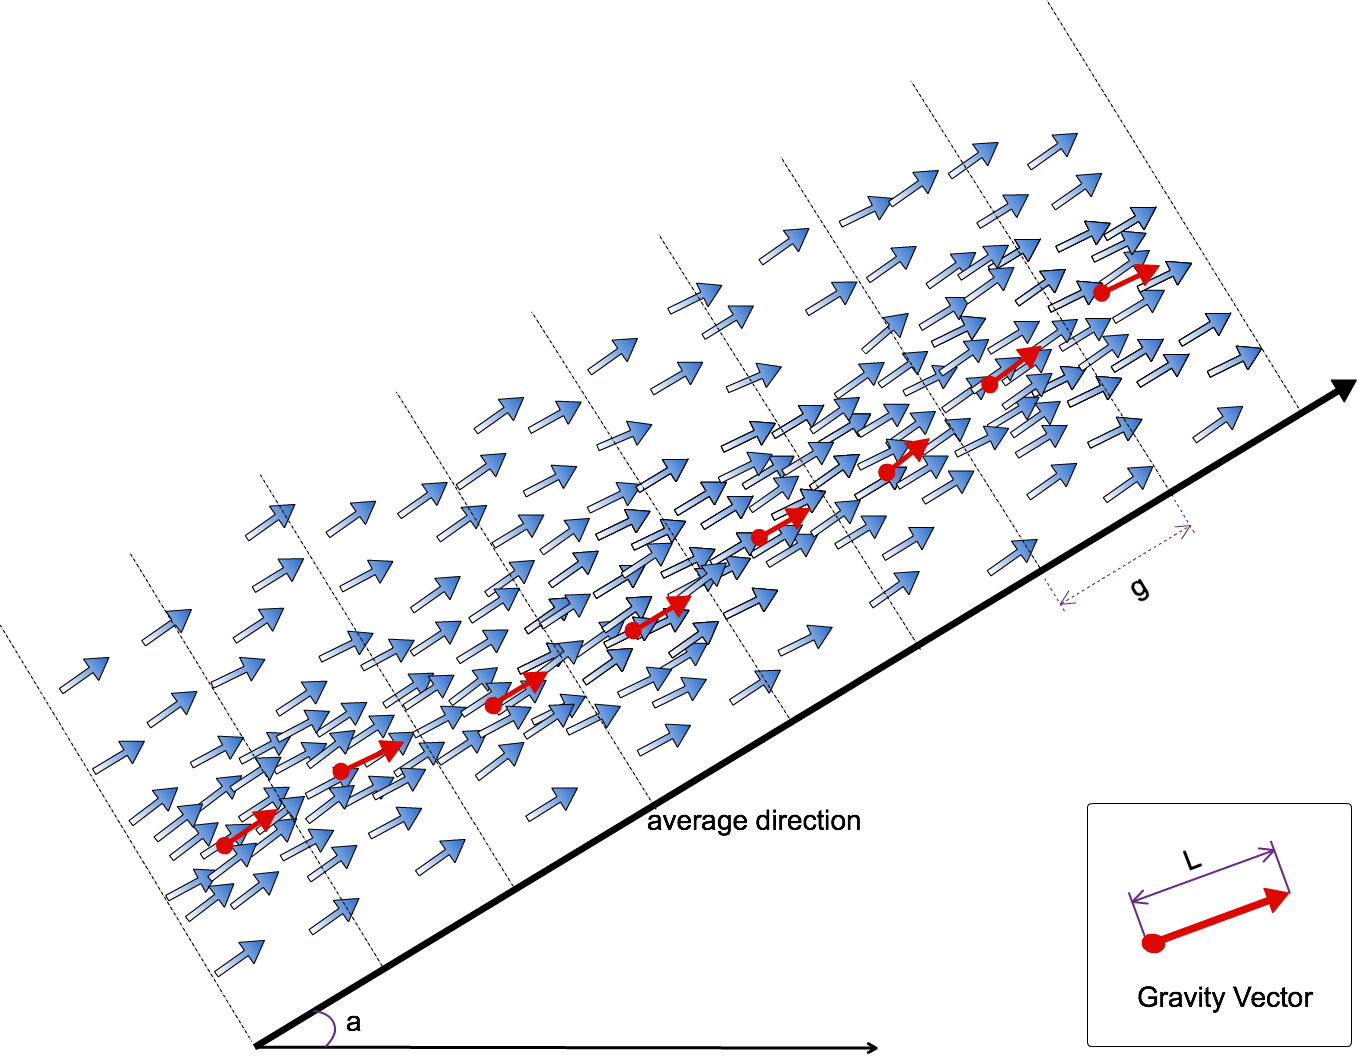
\includegraphics[width=6in]{gravityCalculation.png}%height=8cm
\caption{Calculate Gravity Vectors (GV) for one moving cluster. Blue arrows stand for the trajectory points of the cluster, red arrows are the final Gravity Vectors. The length ($L$) of the GV is the $SOG_{avg}$ of the GV. The width of a grid $g$ is the pre-defined length for partitioning the points.}
\label{fig:gravityPoint}
\end{figure}




A Gravity Vector is extracted by partitioning a cluster into multiple parts, therefore, each cluster can contain multiple Gravity Vectors. Figure \ref{fig:gravityPoint} presents an example of calculating the Gravity Vectors of one cluster. To partition a cluster, a grid width needs to be first determined. The grid width ($g$ in Figure \ref{fig:gravityPoint}) can be decided based on the domain knowledge or multiple experiments' results. Here in this thesis, we choose the length of $eps$ used in Algorithm \ref{algo1} as that of $g$. A Gravity Vector is a vector formed by five features: average COG, average SOG, average Latitude, average Longitude and Median Distance. Then one Gravity Vector $GV_i$ can be denoted by:

%A GV is not a merely centroid of one cluster, it is extracted based on a partition method and thus every cluster can have multiple GVs. 
\begin{equation} 
\label{eq:gvi}
GV_i = <COG_{avg},SOG_{avg},LAT_{avg},LON_{avg},D_{median}>
\end{equation}

As seen in Figure \ref{fig:gravityPoint}, all the blue arrows in the figure are belonging to the same cluster and we can see that all the trajectory points in this cluster have similar COGs (directions). Although it is a bit hard to see the speeds from the figure, we know each point in the cluster has minor SOG variation compared with its neighbors' SOGs. In this example, since the cluster is partitioned into 8 grids, the final output for representing the cluster will be a set of 8 Gravity Vectors. The steps of calculating the Gravity Vectors are as following:

\textbf{Step (1)} Calculate the average COG of the whole cluster and let it be $COG_w$. Note that $COG_w$ is not $COG_{avg}$ in equation \ref{eq:gvi}.

\textbf{Step (2)} Partition all the trajectory points in the cluster along the direction of $COG_w$ by a pre-defined grid width ($g$ in Figure \ref{fig:gravityPoint}). 

\textbf{Step (3)} For each grid of the partitioning results, generate the gravity vector of the grid. \\

In step (3), assume there are $k$ trajectory points in one grid and $TP_i$ is the $ith$ trajectory point, we can calculate the first 4 features using the following 4 formulas (\ref{eq:cog_avg}$-$\ref{eq:lon_avg}). 


\begin{equation} 
\label{eq:cog_avg}
COG_{avg} = \frac{\sum_{i=1}^k TP_i.COG}{k}
\end{equation}

\begin{equation}
\label{eq:sog_avg}
SOG_{avg} = \frac{\sum_{i=1}^k TP_i.SOG}{k}
\end{equation}

\begin{equation}
\label{eq:lat_avg}
LAT_{avg} = \frac{\sum_{i=1}^k TP_i.Latitude}{k}
\end{equation}

\begin{equation}
\label{eq:lon_avg}
LON_{avg} = \frac{\sum_{i=1}^k TP_i.Longitude}{k}
\end{equation}


Then to calculate the last feature $D_{median}$, we should first calculate the distances between all $k$ points in the grid and the average geographical point ($LAT_{avg}$, $LON_{avg}$) generated by formula \ref{eq:lat_avg} and formula \ref{eq:lon_avg}. After this, 
%% MSYD (asymptotically faster method than sorting)
we can apply a linear time complexity algorithm for computing median $D_{median}$ based on Hoare's PARTITION algorithm.


In Lemma \ref{lemma:time_gv}, we present the time complexity of calculating GVs for a cluster.

\begin{lemma}
\label{lemma:time_gv}
The 
%% MSYD
worst
%%
time complexity of calculating a specific cluster's Gravity Vectors is 
%O(nlogn)
O(n), where n is the total number of points in the cluster.
\end{lemma}

\begin{proof}
Assume there are $n$ points in one cluster and the cluster is partitioned into $m$ grids. Step (1) takes O(n) time to calculate the average COG of the whole cluster. Step (2) takes O(n) time to map all the points to the axis of average COG and O(n) time to partition them into $m$ grids. In step(3), to calculate one particular GV for the $i$th grid with $k_i$ points, it takes $O(k_i)$ time to calculate the first 4 features and 
$O(k_i)$
%$O(k_ilogk_i)$ 
time to calculate the median distance 
%
in linear time using one of the algorithms based on the Hoare's partition algorithm \cite{hoare:partition-cacm62}, for example the Blum-Floyd-Pratt-Rivest-Tarjan algorithm \cite{blum:linearSelection-jcss73} that has linear worst time.
 
And this procedure needs to be repeated for $m$ times, the total time for step (3) can be calculated as following:

\begin{eqnarray*}
W(n) = \sum_{i=1}^m O(k_i) = O(n)
%% & = & O( k_1logk_1 + k_2logk_2 + ... + k_mlogk_m) + O(n)\\
%% & < & O( k_1logn + k_2logn + ... + k_mlogn) + O(n) \\
%% & = & O(( k_1 + k_2 + ... + k_m)logn) + O(n) \\
%% & = & O(nlogn) + O(n) \\
%% & = & O(nlogn)
%%%& = & O(n)
\end{eqnarray*} 

%% \begin{eqnarray*}
%% T & = & \sum_{i=1}^m O(k_ilogk_i) + \sum_{i=1}^m O(k_i) \\
%% & = & O( k_1logk_1 + k_2logk_2 + ... + k_mlogk_m) + O(n)\\
%% & < & O( k_1logn + k_2logn + ... + k_mlogn) + O(n) \\
%% & = & O(( k_1 + k_2 + ... + k_m)logn) + O(n) \\
%% & = & O(nlogn) + O(n) \\
%% & = & O(nlogn)
%% \end{eqnarray*} 
 
Thus the pessimistic total time complexity for the whole procedure from step (1) to step (3) is 
O(n).
%%O(nlogn).

\end{proof}

The feature \textbf{Median Distance} can be used to measure the width variance of a moving cluster. The work done by Etienne $et$ $al$ \cite{Etienne12} shows the choice of the statistical decile used to compute the spatio-temporal channel can give a tolerable estimate of this channel's width. However, we use median rather than ninth decile in \cite{Etienne12} to provide a more robust width estimation metric. The distance is not the exact width of the channel, instead, it is a relative distance for outlier detection. More detailed information about how to use the GV for anomaly detection is presented in Chapter \ref{ch:anomaly_detection}.



% Theorem~\ref{theorem-sample} is a sample theorem.

\section{Normal Stopping Areas Extraction}
\label{sec:normal_stopping_model}

In stopping areas, such as ports and wharfs, there may be different types of ships at anchor with zero-velocity or new arriving vessels entering the area with extremely low speed. In this case, vessels can stop with their prows pointing to any directions and change their headings frequently to arrive at the anchorage berths. Therefore, direction is no longer an essential part for analyzing the risk of collision. The possibility of a low-speed vessel colliding with another ship is very low; therefore this situation was excluded from the clustering process. In other words, only when a ship sails with a higher speed than the stopping threshold in a stopping area can we label the data as outlier. So the task of this stage is to identify the locations and geographical shapes of the stopping areas from the historical data set.


Based on the analysis of stopping regions,  the original DBSCAN \cite{DBScan96} algorithm can be employed for stopping points clustering since speed or direction is no longer essential factors. The output is a set of stopping clusters with high density of trajectory points. Intuitively, there is a relatively large number of vessels gathered in each stopping cluster, which indicates the region is a reasonable place for ships to anchor. 

It should be noted that it is common to have both stopping clusters and moving clusters in a specific region at the same time, e.g., a shipping lane can pass through a stopping area. So the phenomenon that a vessel is approaching the port (stopping area) with a low speed is not supposed to be considered abnormal.  Our approach can handle these kinds of issues because both types of clusters can be generated during the normal traffic patterns extraction step and the abnormality of a point will be decided based on both types clusters.
%So in this case we cannot directly determine whether it is abnormal if a trajectory point data has a higher speed than the stopping threshold.

%Although DBSCAN\cite{DBScan96} can generate stopping points clusters, as shown in Figure \ref{LAa},


Although DBSCAN \cite{DBScan96} can generate stopping points clusters, these original clustering results are still not adaptable for the next anomaly detection phase because the relatively large number of points in each cluster may pose serious constraints regarding the computational feasibility. Consequently, just like GV, a similar representative point called  \textbf{Sampled Stopping Point (SSP)} is proposed. Algorithm \ref{algo2} shows the whole procedure for generating the final SSPs given a set of stopping trajectory points in a specific region. 

\begin{algorithm}
\caption{Extract SSP From Stopping Dataset}
\label{algo2}
\begin{algorithmic}[1]
%\Procedure{queryNeighborPoints}{$data$, $P$, $eps$, $MinPts$, $MaxDir$, $MaxSpd$}
\Require The list of the stopping points of the region, $DatasetS$; Reachable distance, $eps$;  Reachable minimum number of points, $MinPts$
\Ensure The list storing the region's SSP, $resultSSP$

\State $StoppingPointsClusters \gets$ DBSCAN($DatasetS$, $eps$, $MinPts$)\Comment{see DBSCAN algorithm in \cite{DBScan96}}
\State $resultSSP \gets$ empty list
\For {each cluster $C$ in $StoppingPointsClusters$} %\Comment{first extract the 4 border values of cluster C}
    \State{$lat1, lat2$ $ \gets$ minimum and maximum of all the points' Latitude values in cluster $C$}
    %\State{$lat2 \gets$ maximum of all the points' Latitude values in cluster $C$}
    \State{$lon1, lon2 \gets$ minimum and maximum of all the points' Longitude values in cluster $C$}
    %\State{$lon2 \gets$ maximum of all the points' Longitude values in cluster $C$}
    
    \Comment{estimate the sample size for cluster $C$}
    \State{$area \gets \left|(lat1-lat2)*(lon1-lon2)\right|$}
    \If {$area$ = 0}
        \State{$sample\_size \gets$ 1}
    \Else 
         \State{$sample\_size \gets$ Ceiling($area$/($\pi*eps^2$))}
    \EndIf
    \Comment{sample the stopping area points}
    \State{$count \gets$ 0}
    \While {$count < sample\_size$}
        \State{randomly select one point $P$ from cluster $C$}
        %\If{ $P$ is near one of the $resultSSP$}
        %    \State{continue}
        %\Else
        \If{ $P$ is far from all points in $resultSSP$}
            \State{$resultSSP$.add($P$)}
            \State{$count$++}
        \EndIf    
    \EndWhile
\EndFor
\State \textbf{return} $resultSSP$
\end{algorithmic}
\end{algorithm}

\begin{figure}[!htb]
\centering
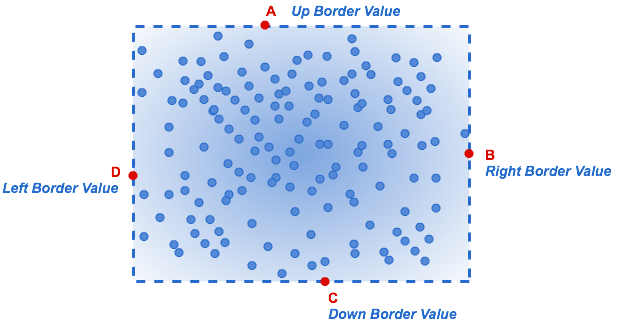
\includegraphics[width=5.5in]{borderValue.png}
\caption{Border Values of a stopping cluster}
\label{fig:border_value}
\end{figure}


As shown in Algorithm \ref{algo2}, stopping points are first clustered by the DBSCAN \cite{DBScan96} algorithm (line 1). The same parameters ($eps$ and $MinPts$) used by DBSCANSD (Section \ref{sec:normal_moving_model}) are still employed in this stopping areas extraction phase. Then the algorithm starts to generate the SSPs for every cluster. The key idea about SSP is to find the representative points that reflect the shapes and locations of the stopping areas. But before extracting the points from the clustering results, an estimation of the number of SSPs needs to be conducted. To address this issue,  lines 4$-$10 first estimate the area of the region and then calculate the sample size. Lines 4 and 5 calculate the four border values of the cluster. Border values are extreme values of one cluster. Figure \ref{fig:border_value} shows an example of border values in a stopping cluster. In Figure \ref{fig:border_value}, 4 border points A-D are in red color and Up Border Value is the maximum of all points' Latitude values while Down Border Value is the minimum. Then B and D can be extracted in a similar way as A and C. Any two or three of them (or even all the four points) can be the same point. It is noteworthy that if one cluster crosses the Greenwich meridian, the way to calculate the two border values, $lon1$ and $lon2$, will be changed. 

\begin{figure}[!htb]
\centering
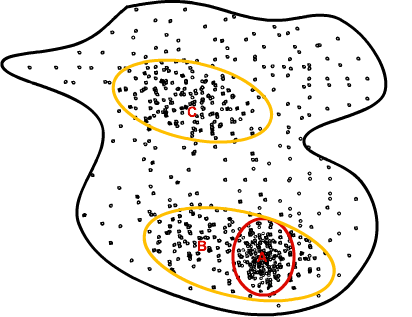
\includegraphics[width=4.5in]{stopExample.png}
\caption{An example of a stopping area where simple random sampling cannot work. There are three regions (A,B and C) with higher density than the whole area's average density.}
\label{fig:stopping_area}
\end{figure}

After extracting the 4 border values, the area of the border (blue border lines shown in Figure \ref{fig:border_value}) is calculated. With this area result and the $eps$ used for clustering, the sampling number is estimated (lines 6$-$10). Lastly, we use a random selection strategy to sample the stopping points. However, there still exists some sub-regions with higher density of points compared with other sub-regions in the same cluster and as a result,  random selection tends to select points from these higher-density micro-regions. 

An example is shown in Figure \ref{fig:stopping_area}. Figure \ref{fig:stopping_area} shows a stopping area with three higher densely sub-regions and all the black points are the stopping points of the clustering result. We can see that the sub-region $A$ has the highest density while $B$ and $C$ have relatively lower density which are still higher than the whole average. So in this example, if we simply employ a random selection technique, the majority of the final points shall be extracted from region $A$ and then regions $B$ and $C$. There might be only a limited number of points that are sampled from the rest of the whole stopping area, which is not supposed to happen in terms of representing the whole area's shape.  As a consequence, we need to modulate the  sampling process to stratified sampling to give each sub-region equal probability to be selected. This can be easily done with lines 11$-$16; the distance condition in line 14 can be defined by $eps$ as well. The algorithm has linear time complexity.

Thus, with the Gravity Vectors and Sampled Stopping Points extracted from the moving and stopping AIS data separately, the anomaly detection task can be conducted, the techniques for which are presented in the next chapter.

%%%%%%%%%%%%%%%%%%%%%%%%%%%%%%%%%%%%%%%%%%%%%
%%%%%%%%%%%%%%%%%%%%%%%%%%%%%%%%%%%%%%%%%%%%%


\chapter{Anomaly Detection}
\label{ch:anomaly_detection}

In this chapter, we present our anomaly detection model. Similar to the normal traffic pattern extraction model, we also treat stopping and moving separately. A ship trajectory in a particular area, especially in the near-port areas, can consist of both stopping points and moving points. Hence, given one incoming trajectory data set (one sequence of trajectory points with same identification), every point in this trajectory should first be labeled as stopping or moving according to the SOG threshold (0.5 knots) and then be checked for abnormality.  In the following part of the section, three division distances are first presented in Section \ref{sec:three_division_distances} and then our abnormal detection model is introduced in Section \ref{sec:anomaly_detection_model}.

\section{Three Division Distances}
\label{sec:three_division_distances}

In this section,  three specialized division distances are proposed to label every data point: Absolute Division Distance (ADD), Relative Division Distance (RDD) and Cosine Division Distance (CDD). $ADD$ is employed in the stopping points abnormality detection phase while $RDD$ and $CDD$ are used for the moving part. The definitions of the three division distances are given in the following. Here we use \textbf{target point}s to represent the points of a new coming trajectory to be labeled.\\

The \textbf{Absolute Division Distance} between a target point $P_t$ and a Sampled Stopping Point $P_s$ is defined as:
\begin{equation}
\label{eq:add}
D_{absolute} = \\
Distance((P_t.Lat,P_t.Lon),(P_s.Lat,P_s.Lon))
\end{equation}
% \begin{equation}
% \label{eq:add}
% \resizebox{\hsize}{!}{$D_{absolute} = Distance(<P_t.Lat,P_t.Lon>,<P_s.Lat,P_s.Lon>)$}
% \end{equation}



As can be seen in Definition \ref{eq:add}, ADD is actually the Geographical Distance \cite{gpsDistance} between %the two geographical points formed by the 
Latitude and Longitude values of the target point($P_t$) and the sampled stopping point($P_s$). %The reason for naming it is to distinguish it from the Relative Division Distance (Equation \ref{eq:rdd}). 

The \textbf{Relative Division Distance} between a target point $P_t$ and a Gravity Vector $GV$ is defined as:

\begin{equation}
\label{eq:rdd}
D_{relative} = \frac{Distance((P_t.Lat,P_t.Lon),(GV.Lat,GV.Lon))}{GV.MedianDistance}
\end{equation}

% \begin{equation}
% \label{eq:rdd}
% \resizebox{\hsize}{!}{$D_{relative} = \frac{Distance(<P_t.Lat,P_t.Lon>,<GV.Lat,GV.Lon>)}{GV.MedianDistance}$}
% \end{equation}

%where $MedianDistance$ is the MedianDistance feature of GV.

For moving trajectory points, we adopt RDD ($D_{relative}$) rather than ADD ($D_{absolute}$) because the normal moving lanes could have different widths according to their surrounding geographical environment. The routes in a narrow strait can be more cramped than those in the open sea. Relative distance, the ratio of a point's distance from the centroid to the median distance of all the points in one cluster from the centroid, is one efficient metric in clustering-based approaches for detecting outliers \cite{PangNing05}. We replace the centroid of each cluster with our Gravity Vectors, which can be regarded as surrogates for a centroid when we only consider Longitude and Latitude.
%Therefore, we can replace the centroid with our Gravity Vectors because GVs can be regarded as another type of centroids if we only consider Longitude and Latitude.
As stated in \cite{bigdata2014} and previous section, every cluster can have more than one GV, in which case the median distance %in Equation \ref{eq:gvi} 
of one GV
can be used to measure the width variance of a moving cluster. Another work that confirms this approach is presented by Etienne $et$ $al.$ \cite{Etienne12} in which it is shown that
%Besides work done by Etienne $et$ $al$\cite{Etienne12} also shows
the choice of the statistical decile used to compute the spatio-temporal channel can give a tolerable estimate of this channel's width.\\

The next division distance is CDD, which is employed to involve direction and speed of moving objects. The \textbf{Cosine Division Distance} between a target point $P_t$ and a Gravity Vector $GV$ is defined as:
% \begin{equation}
% \label{eq:cdd}
% \resizebox{0.5\hsize}{!}{$D_{cosine} = \cos\alpha\times\frac{\left|{SOG(x)} \right|}{\left|{SOG(y)}\right|}$}
% \end{equation}

\begin{equation}
\label{eq:cdd}
D_{cosine} = \cos\alpha\times\frac{min(P_t.SOG,GV.SOG)}{max(P_t.SOG,GV.SOG)}
\end{equation}
\begin{quote}
where:

 $\alpha$ is the angle between the two directions, that is, the difference between $P_t$'s COG and $GV$'s COG. \\
\end{quote}

% \begin{equation}
% \label{eq:cdd}
% D_{cosine} = \cos\alpha\times\frac{\left|{SOG(x)} \right|}{\left|{SOG(y)}\right|}
% \end{equation}
% \begin{quote}
% where:

% (1) $\alpha$ is the angle between two directions, that is, the difference between $P_t$'s COG and $GV$'s COG.

% (2)$\left| {SOG(x)} \right|\leq\left| {SOG(y)} \right|$

% (3)$\left| {SOG(x)} \right|$ and $\left| {SOG(y)} \right|$ are the two speeds of $P_t$ and $GV$. $x$ can be either $P_t$ or $GV$, decided by condition (2).
% \\
% \end{quote}


The intuition behind CDD is to combine the angle ($\leq$ 180$^\circ$) between the two directions (angle $\alpha$ is defined by COG differences between $P_t$ and $GV$) and the difference between the two speeds. Figure \ref{fig:abnormal_cogsog} shows two abnormal cases that consider COG and SOG. In Figure \ref{fig:abnormal_cogsog}(a), we can see that the speeds of the two vectors are in the same length $L$ while the angle $a$ is too large. This could be explained as a ship crossing a normal lane in a nearly opposite direction, which may cause a collision. In Figure \ref{fig:abnormal_cogsog}(b), the speed of the target point $P_t$ is much lower than $GV$'s although they have similar COG. In this case, the slowly sailing vessel may also be in a high risk of collision in relation to other ships moving at a normal rate of speed. As a consequence, Cosine Division Distance (CDD) is proposed. It can be easily seen that $cos$ $\alpha$ accounts for the angles' difference and the ratio between two SOGs can reflect the speeds' difference. 

\begin{figure}[!htb]
\centering
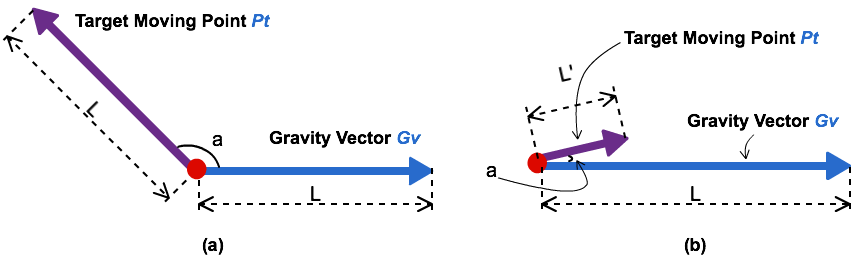
\includegraphics[width=14cm,height=5cm]{abnormalSpeedDirection.png}
\caption{Two Abnormal Cases after considering COG and SOG}
\label{fig:abnormal_cogsog}
\end{figure}



The Cosine Division Distance proposed in this work combines both COG and SOG in its calculation. A possible alternative is to calculate the distance of each component separately and then check the normality, but this alternative may increase the misclassification error. One example is presented in Figure \ref{fig:abnormal_cosine}. In this scenario, it is assumed that a certain point $P_t$ is in the middle of two different grids belonging to different clusters. If this approach of separately calculating each component is employed, the target point, $P_t$, will first be considered normal with respect to $G_v$' on the basis of direction, and also with respect to $G_v$ on the basis of length (value of speed).
%because it has a similar direction as $G_v$' and then be considered normal too because the length (speed) of it is same as that of the other gravity vector ($G_v$).
However, $P_t$ is an abnormal point because it is in the direction of $G_v$', but with a much faster speed.

%One might argue that why don't we separate CDD into two independent parts (COG and SOG) instead of using this combination distance. The basic reason is that for a specific area, even a specific point, there can be multiple moving (or stopping) clusters with different directions and speeds. Then if we separate CDD, we have to compare COG or SOG first and the other one next, which can cause misclassification. For instance, in Figure \ref{fig:abnormal_cosine}, there are two moving clusters in the area and a target point to be labeled. If we use the separate method, the target point $Pt$ will be first considered normal because it has a similar direction as $Gv'$ and then be considered normal too because the length (speed) of it is same as that of the other gravity vector($Gv$). However, $Pt$ is an abnormal point because it is in the direction of $Gv'$ with a much faster speed than the normal cluster's. 
\begin{figure}[!htb]
\centering
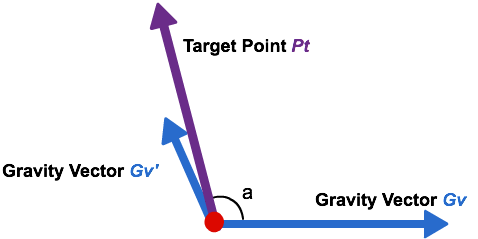
\includegraphics[width=8cm]{cosine.png}
\caption{One case that the simple combination of the two division distances cannot work. There are two moving clusters in one specific area and the two clusters are with two different average COGs. }
\label{fig:abnormal_cosine}
\end{figure}

\section{Anomaly Detection Model}
\label{sec:anomaly_detection_model}

After having the three division distances defined, we can present our anomaly detection model. %Algorithm \ref{algo3} shows this straightforward method. 

\begin{algorithm}
\caption{Detect abnormality of the target trajectory}
\label{algo3}
\begin{algorithmic}[1]
\Require (1) The target trajectory dataset, $D$; (2) The lists of Sampled Stopping Points and Gravity Vectors from the previous model, $SSP$ and $GV$; (3) Three thresholds, $add\_threshold$, $rdd\_threshold$ and $cdd\_threshold$
\Ensure The abnormality rate, $abnormality$

\State Separate D into two sub-datasets based on the speed threshold, moving dataset $D\_m$ and stopping dataset $D\_s$
\State Initialize all labels of points in $D\_m$ and $D\_s$ as Normal

\Comment{label stopping points of the target trajectory}
\For {each data point $S$ in $D\_s$} 
    \State{$ADD\_s$ $\gets$ minimum(ADD($S$,$SSP$)) }
    \If{$ADD\_s > add\_threshold$}
        \State{$S.label$ $\gets$ Abnormal}
    \EndIf
\EndFor

\Comment{label moving points of the target trajectory}
\For{each data point $M$ in $D\_m$}
    \State{$RDD\_m \gets$ minimum(RDD($M$,$GV$))}
    \If{$RDD\_m > rdd\_threshold$}
        \State{$M.label \gets$ Abnormal}
    \Else
        \State{$CDD\_m \gets$ maximum(CDD($M$,$GV$))}
        \If{$CDD\_m < cdd\_threshold$}
            \State{$M.label \gets$ Abnormal}
        \EndIf
    \EndIf
\EndFor
\State{$count\_ab$ $\gets$  the number of the abnormal points in $D$}
\State{$count\_all \gets$ the total number of all points in $D$}
\State{$abnormality \gets count\_ab/count\_all$}

\State \textbf{return} $abnormality$
\end{algorithmic}
\end{algorithm}

As shown in Algorithm \ref{algo3}, the anomaly detection process is completed in two steps. Lines 3-6 employ ADD to label the stopping points of the trajectory and Lines 7-14 use RDD and CDD to decide the moving points' labels. Lastly, the ratio of abnormal points to the number of all points is returned as the value of abnormality (Lines 15-18). The abnormality can be interpreted as a confidence ratio in a trajectory point being abnormal and it is beneficial for the end users to  choose a level of confidence while retrieving the abnormal results of the whole system.

This algorithm requires three thresholds as inputs, which can be estimated through experiments. In this work, we first take out one month of data in a specific area and calculate all the division distances, then select specific values based on distribution and quartile analysis. 

\begin{figure}[!hp]
\centering
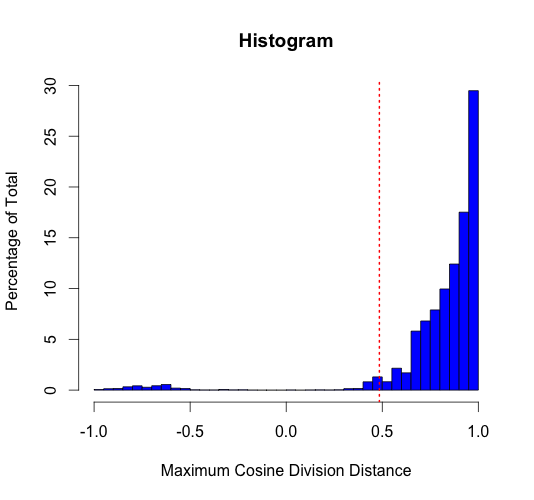
\includegraphics[width=9cm]{hist.png}
\caption{The maximum CDD distribution in the area of Juan de Fuca Strait.}
\label{fig:maxiCDD}
\end{figure}

\begin{figure}[!hp]
\centering
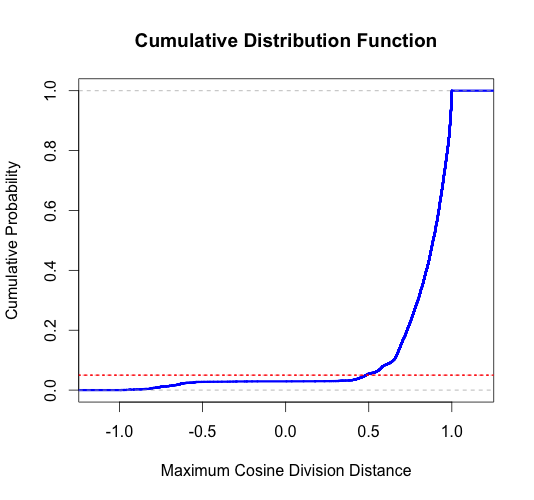
\includegraphics[width=9cm]{cdf.png}
\caption{The Cumulative Distribution Function of the maximum CDD in the area of Juan de Fuca Strait.}
\label{fig:cdf}
\end{figure}

Figure \ref{fig:maxiCDD} shows the distribution of the maximum CDD of moving points in the area of Juan de Fuca Strait. Figure \ref{fig:cdf} illustrates the CDF (Cumulative Distribution Function) of the maximum CDD in the area. The red dotted line in Figure \ref{fig:maxiCDD} is the 5$\%$ separation line, which means the percentage of all the CDDs not greater than the separation coordinate is 5$\%$. Similarly, in Figure \ref{fig:cdf}, the red dotted line is also a 5$\%$ separation line and we can see the corresponding coordinate in y-axis is 0.05. It is obvious that over 90$\%$ of the data points' CDD are greater than 0.5. Thus, in this case, we can choose 0.5 or a smaller value as the CDD threshold for this area and then when a new trajectory dataset is given, we can use this value as the basis for anomaly detection.







\chapter{Evaluation}
\label{ch:evaluation}
In this chapter, experiments are done to evaluate the effectiveness of the proposed approach. First, to evaluate the normal traffic patterns extraction model, regions of Juan de Fuca Strait (Section \ref{sec:exp_1.1}) and Los Angeles Long Beach (Section \ref{sec:exp_1.2}) are selected and the results are presented in Section \ref{sec:exp_1}. Then in Section \ref{sec:exp_2}, we conducted two other experiments in the same region of Juan de Fuca Strait. The first one is conducted with the non-labeled data while the second one is done after labelling the data. The results of the first experiment (Section \ref{sec:exp_2.1}) are  shown  visually  and  the  second  experiment (Section \ref{sec:exp_2.2}) compares our model’s results with the labels by the expert.

\section{Normal Traffic Patterns Extraction Model}
\label{sec:exp_1}
In this section, we evaluate the effectiveness of our maritime normal patterns detection model in two regions. The data set contains non-anonymized messages from ships in the region of Juan de Fuca Strait and the region of Los Angeles Long Beach. The movement rules for port areas defined by IMO extracted from the IMO publication \cite{anabook} are shown in Figure \ref{fig:jdfk_pic} and \ref{fig:la_pic}. Evaluation of the normal patterns detection model is related to the problem of evaluating clusters quality and this is always not a trivial task. Our strategy is to use our approach to generate the lanes and then compare the results with these rules.
%The methodology is applied to data collected from a near port strait, JUAN DE FUCA STRAIT, the entrance of which lies between Cape Flattery (\ang{48;23;}N.,\ang{124;44;}W.) and Carmanah Point (\ang{48;37;}N.,\ang{124;45;}W.).

 
\subsection{Juan de Fuca Strait}
\label{sec:exp_1.1}
The Strait of Juan de Fuca separates the south coast of Vancouver Island from the north coast of State of Washington. The entrance of it lies between Cape Flattery (\ang{48;23;}N.,\ang{124;44;}W.) and Carmanah Point (\ang{48;37;}N.,\ang{124;45;}W.) \cite{juandefuca}. Figure \ref{fig:jdfk_pic} shows a map of this area and the predefined rules for it.

\begin{figure}[!htb]
\centering
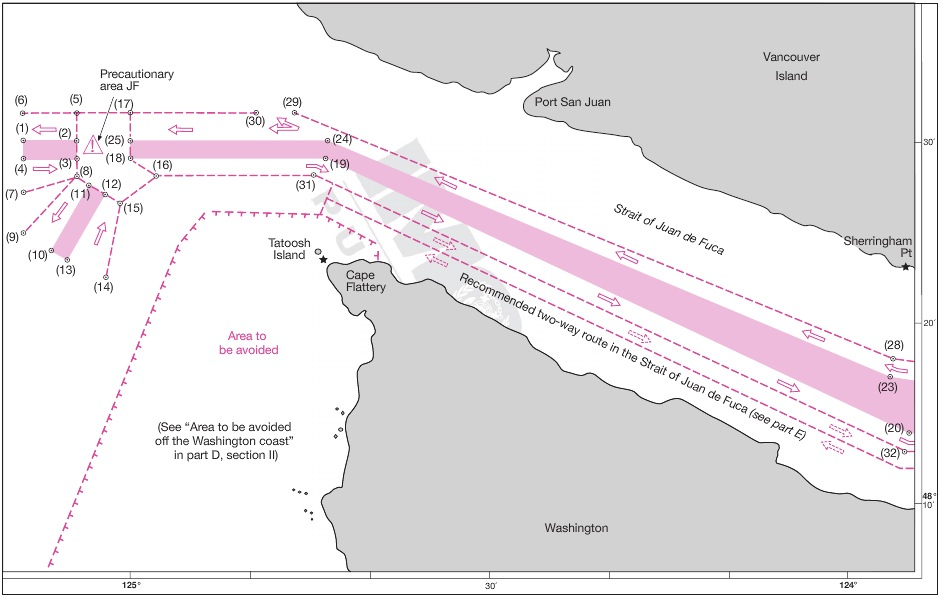
\includegraphics[width=4.9in,height=3.4in]{jdfk_pic.png}
\caption{Juan de Fuca Strait and its approaches (west) \cite{anabook} }
\label{fig:jdfk_pic}
\end{figure}

The data set prepared for this experiment is two-months of trajectory data from November 1 to December 31 in 2012. It consists of 67,850 trajectory points. The whole dataset is not used; instead 46,000 records (40,000 moving points and 6,000 stopping points distinguished by the SOG threshold 0.5 knot) are selected randomly.

%below is useful for the error message: Dimension too large
%\renewcommand\ <at> makefnbreak{\hspace{2em}}

\begin{figure}[!htb]
\centering
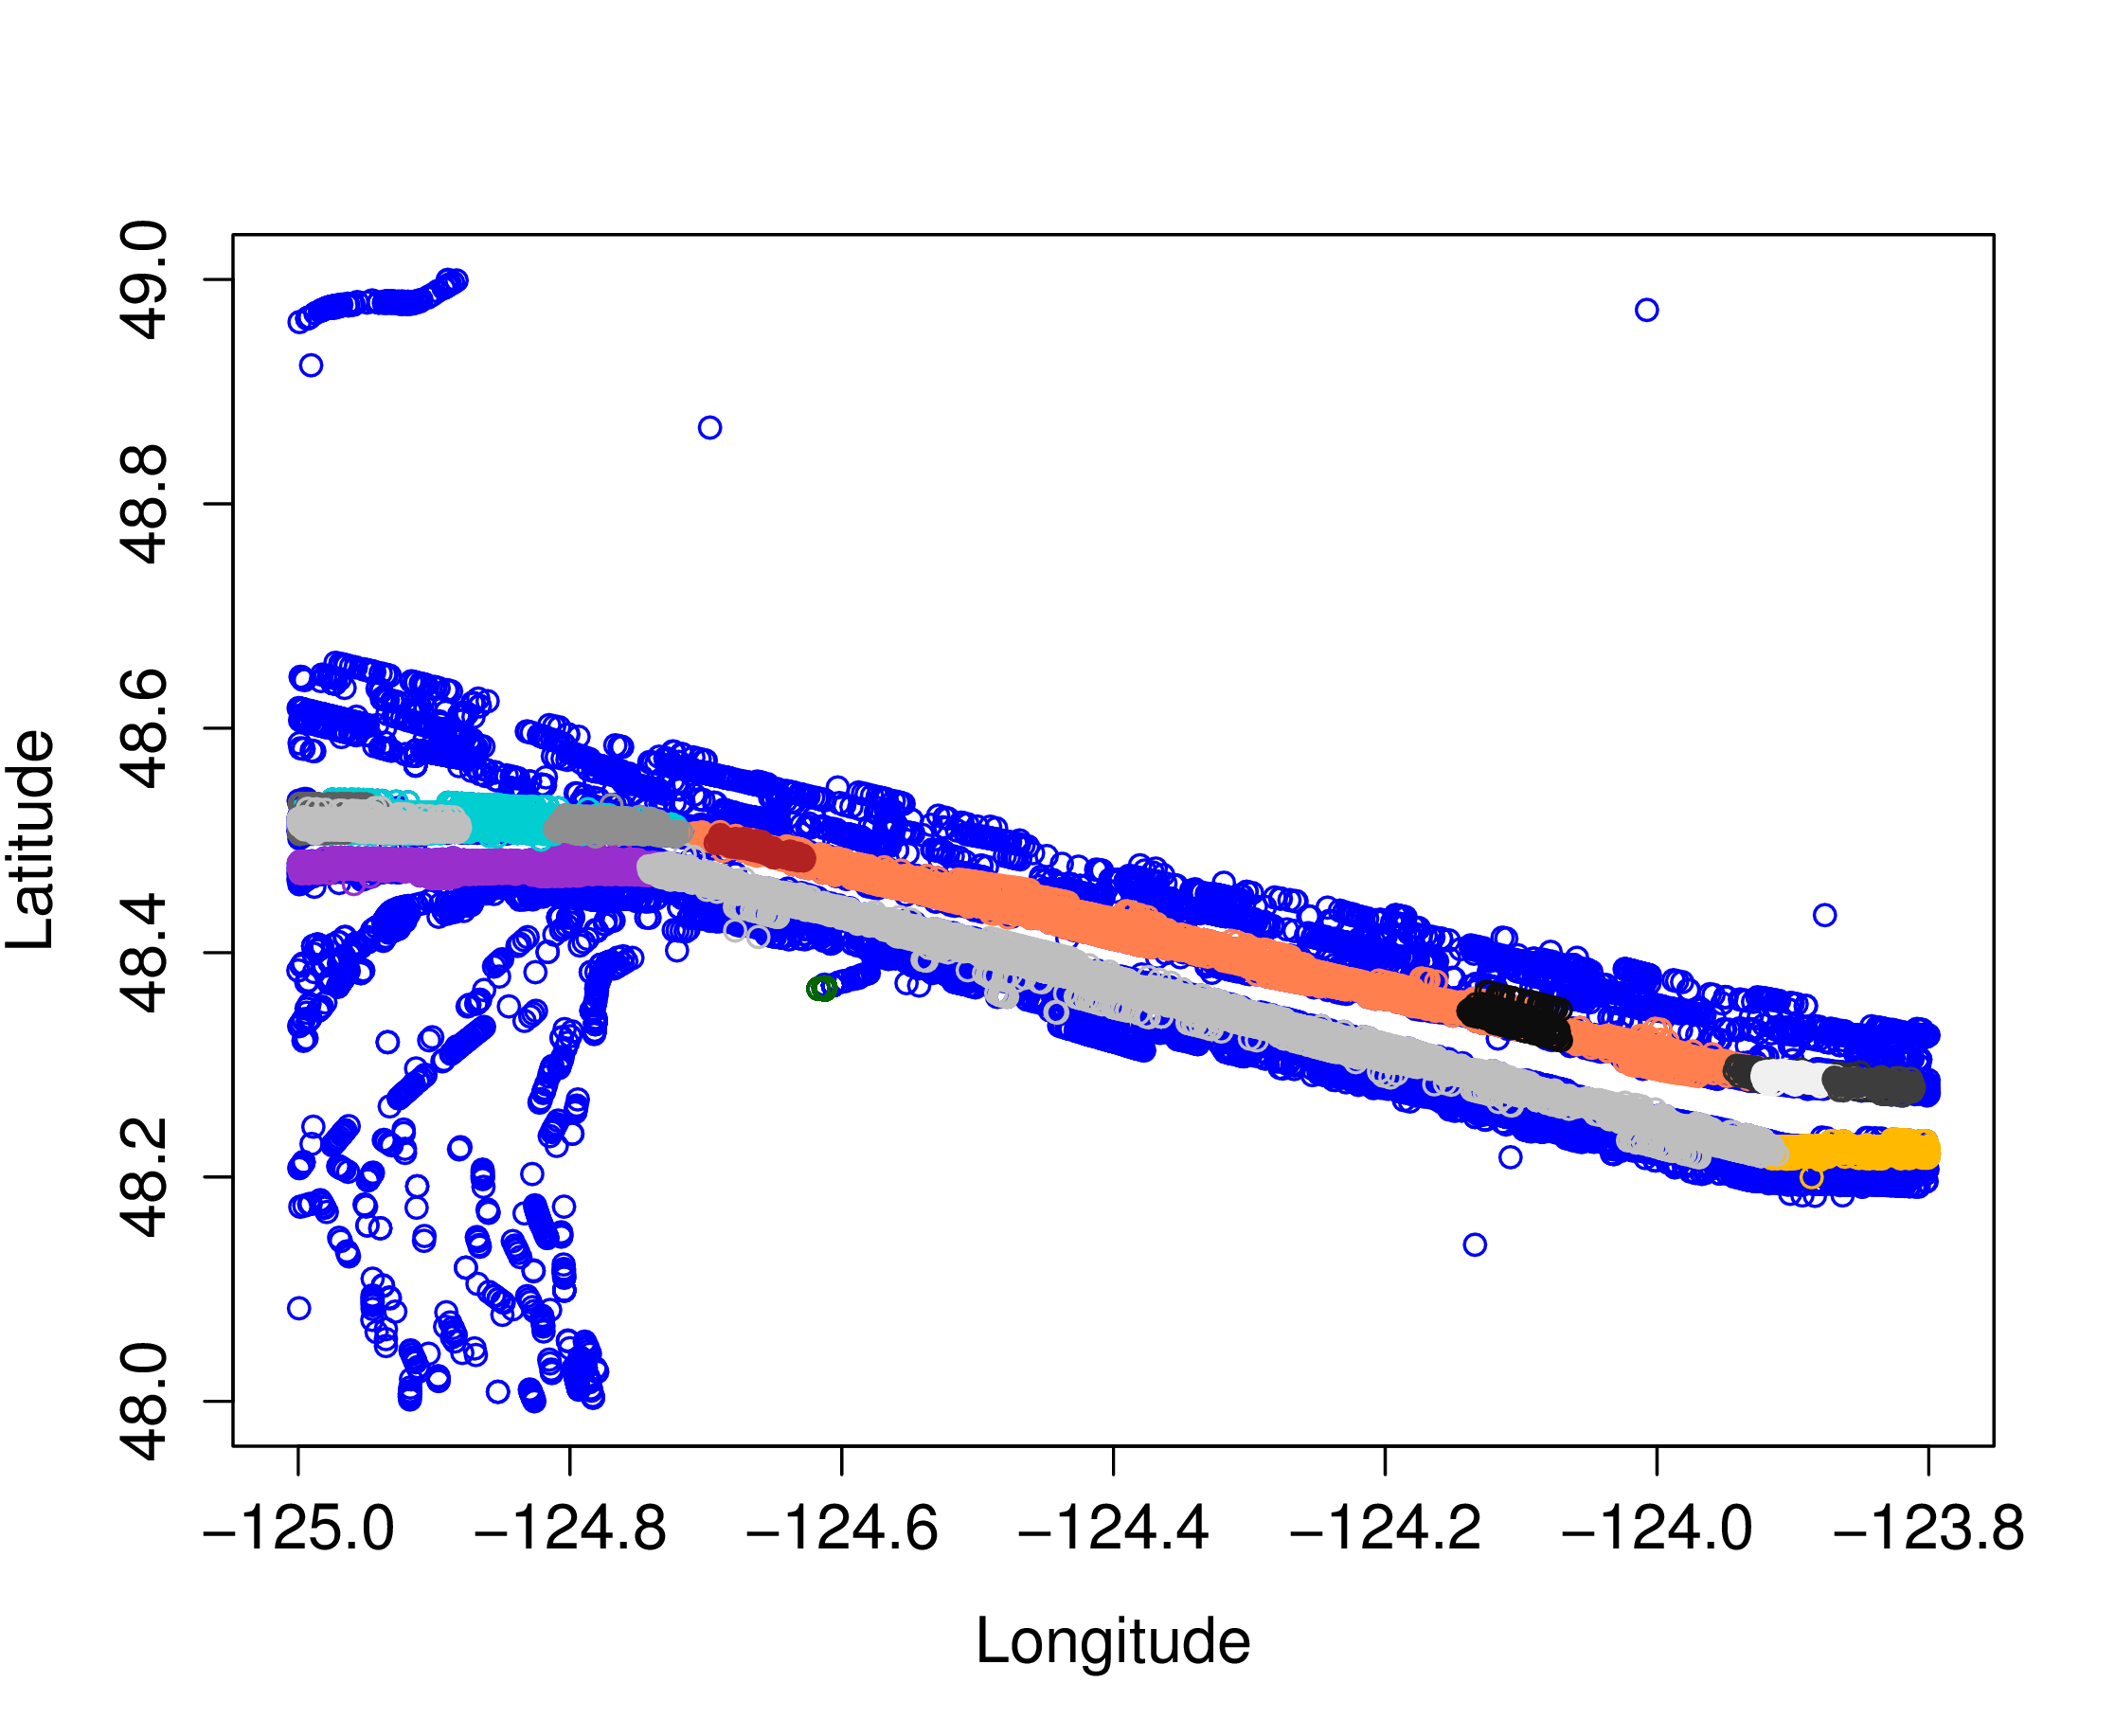
\includegraphics[width=5in]{clusterResultJDFK.png}
\caption{The clustering results of JUAN DE FUCA STRAIT area. Points in blue color are the noise. Other different colors stand for different clusters. The cluster in dark green is a stopping cluster. }
\label{fig:jdfk_cluster}
\end{figure}

After applying the two clustering algorithms, 14 different clusters including 13 moving clusters and 1 stopping cluster are extracted. The result can be seen in Figure \ref{fig:jdfk_cluster}. Points in blue are the original traffic points while others are the cluster points. The size (total number of the points composing the clusters) of moving clustering results is 20,817 while that of the stopping cluster is 4,800.


\begin{figure}[!htb]
\centering
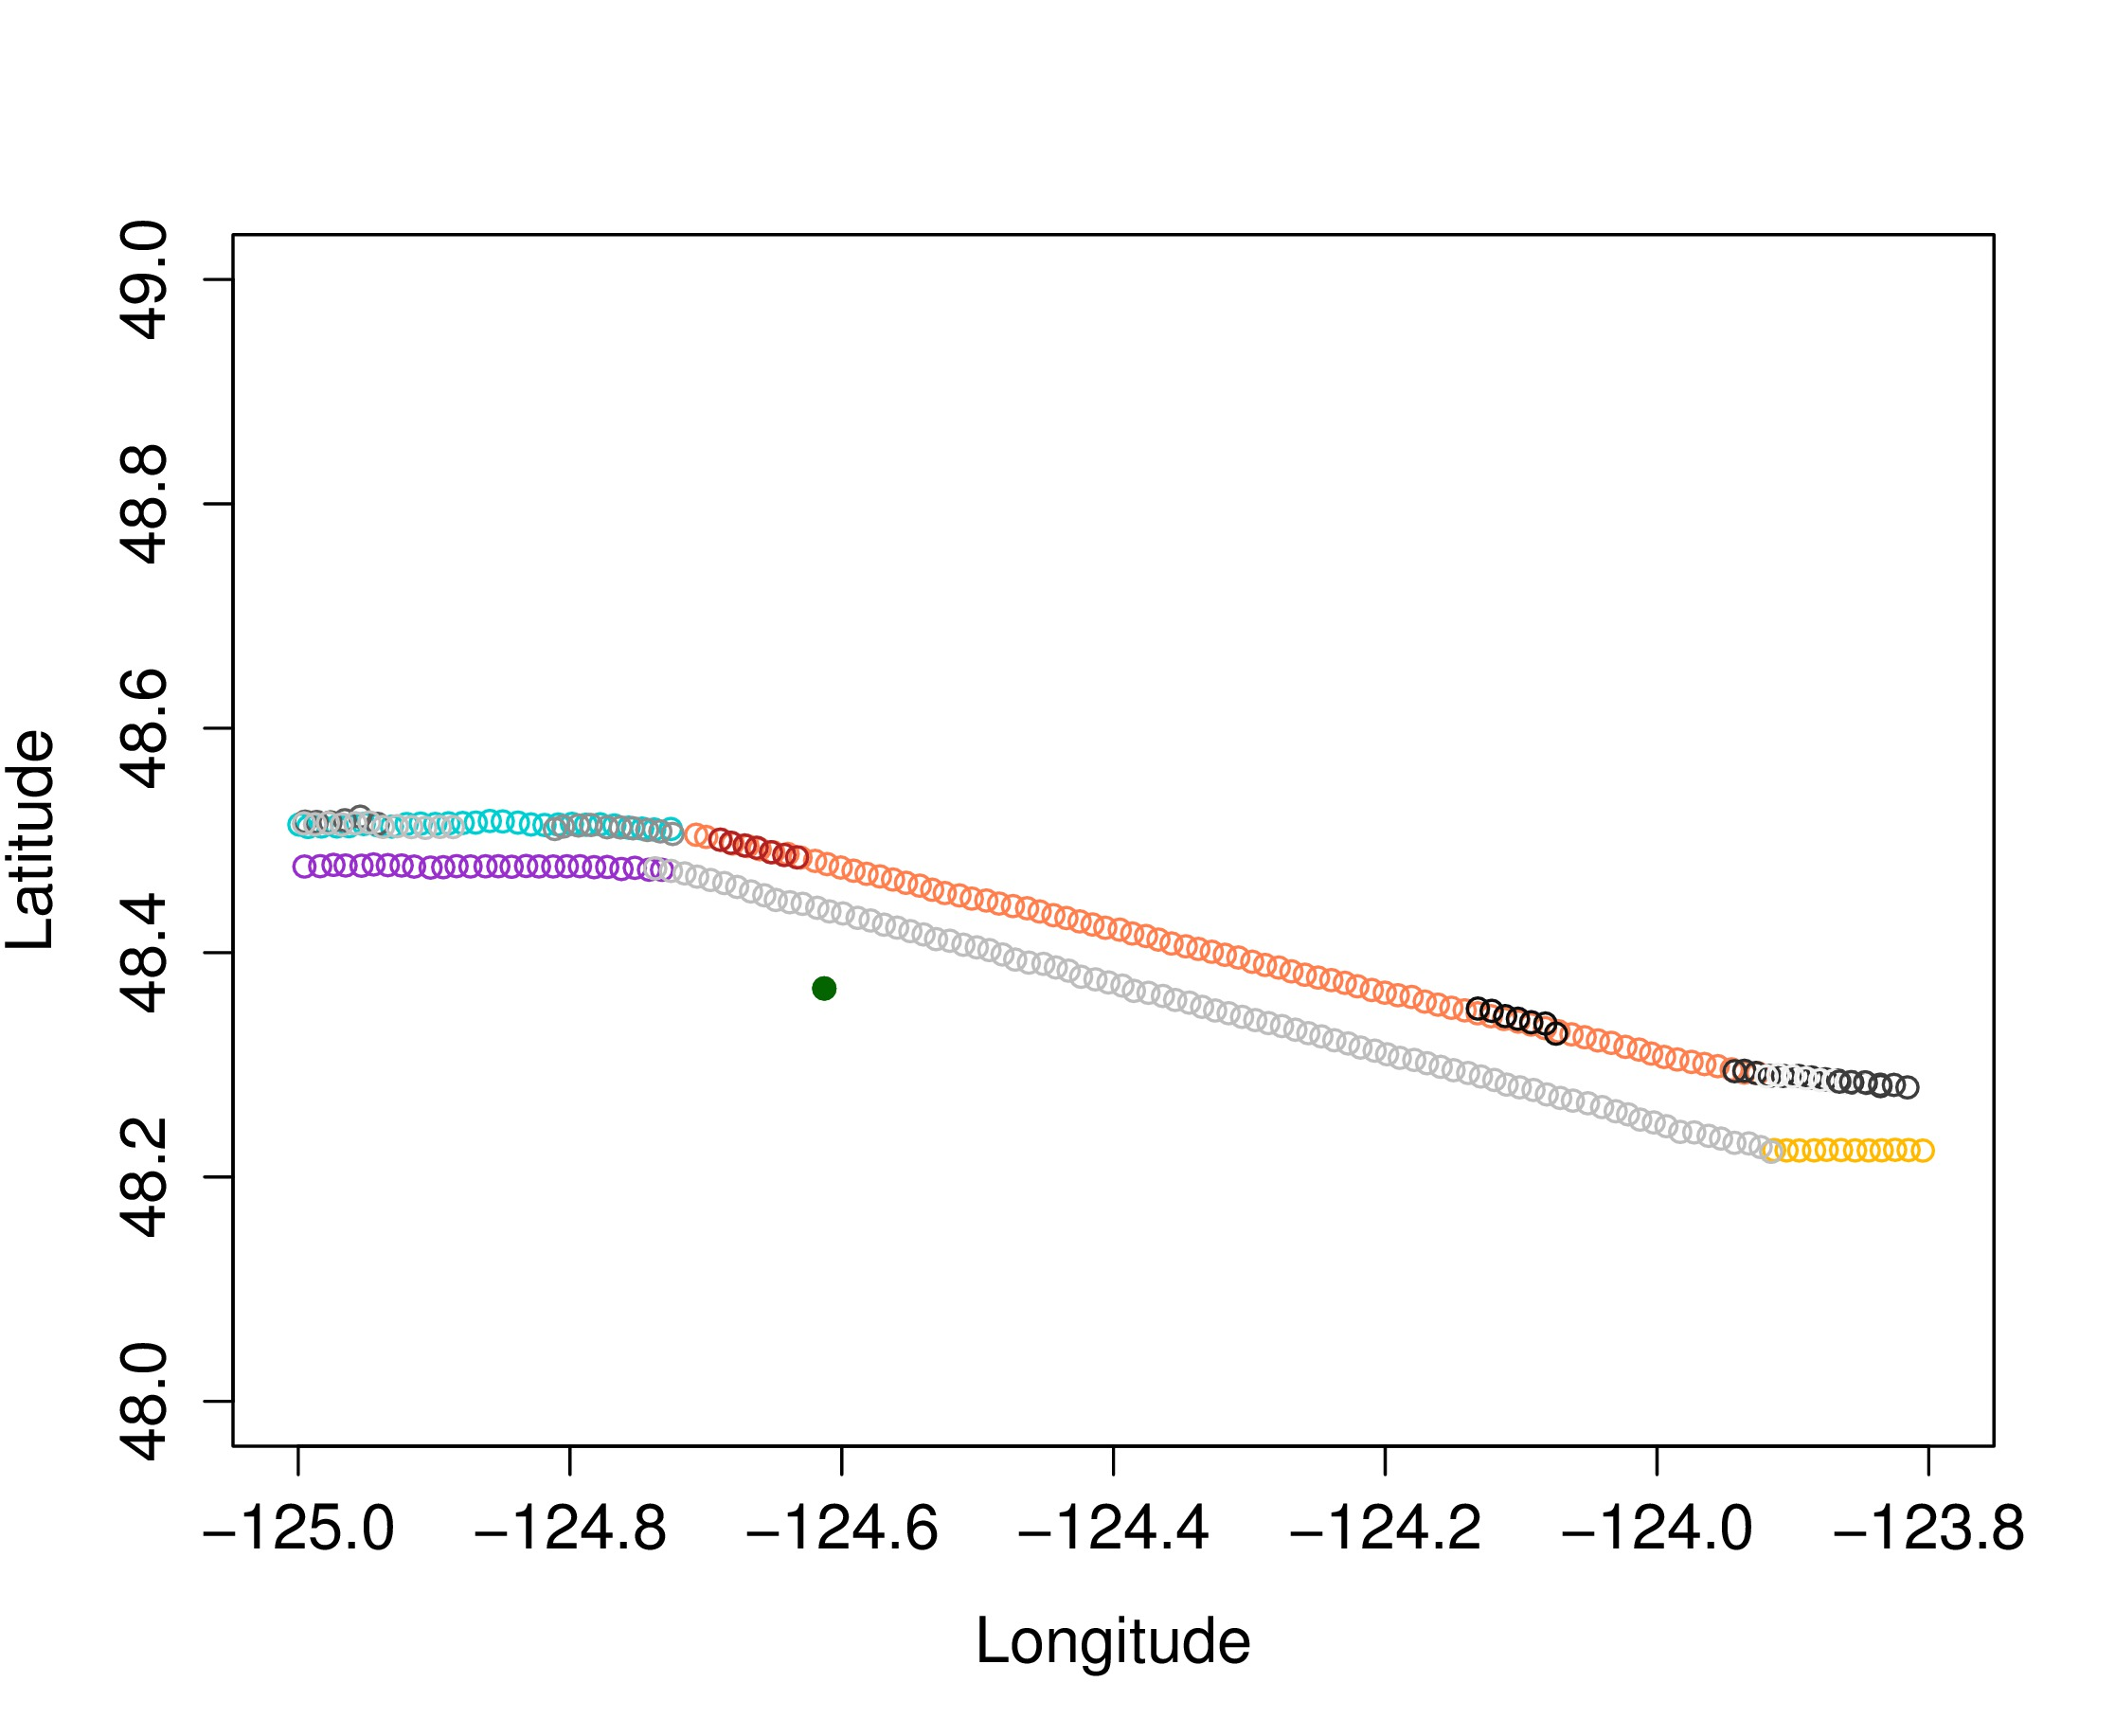
\includegraphics[width=5in]{clusterGV.jpg}
\caption{The Gravity Vectors and Sampled Stopping Points extracted from the clusters in Juan de Fuca Strait area.}
\label{fig:jdfk_gv}
\end{figure}





Figure \ref{fig:jdfk_gv} shows the gravity vectors of the moving clusters and the sampled stopping point of the stopping cluster. After this extraction phase, only 302 points are generated which include 301 GVs and only one SSP. From the two figures we can see that the clustering results can reflect the traffic trends in this strait and the GVs as well as the SSP can represent the clustering results too.

\begin{figure}[!htb]
\centering
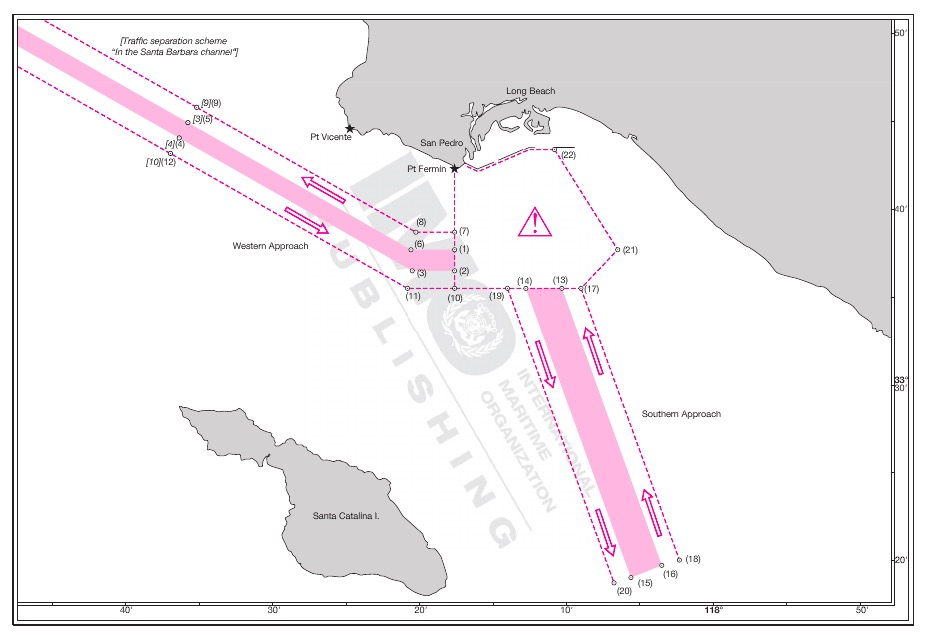
\includegraphics[width=4.6in]{la_pic.png}
\caption{Map of Los Angeles Long Beach and the navigation rules defined \cite{anabook}}
\label{fig:la_pic}
\end{figure}

\subsection{Los Angeles Long Beach}
\label{sec:exp_1.2}
The approach has also been tested in the area of Los Angeles Long Beach, where the traffic is more complicated and heavier. Figure \ref{fig:la_pic} shows a map of the area with two rules defined. In this experiment, the same period (November 1 to December 31 in year 2012) dataset has been prepared. There are 327,694 records (99,937 moving points and 227,757 stopping points) in this dataset. We adopt all the moving points in this dataset for moving clusters generation and the first 20,000 stopping points for stopping area generation.

\begin{sidewaysfigure}
    \centering
    \subfigure[Stopping clusters by DBSCAN \cite{DBScan96} ]{\label{LAa}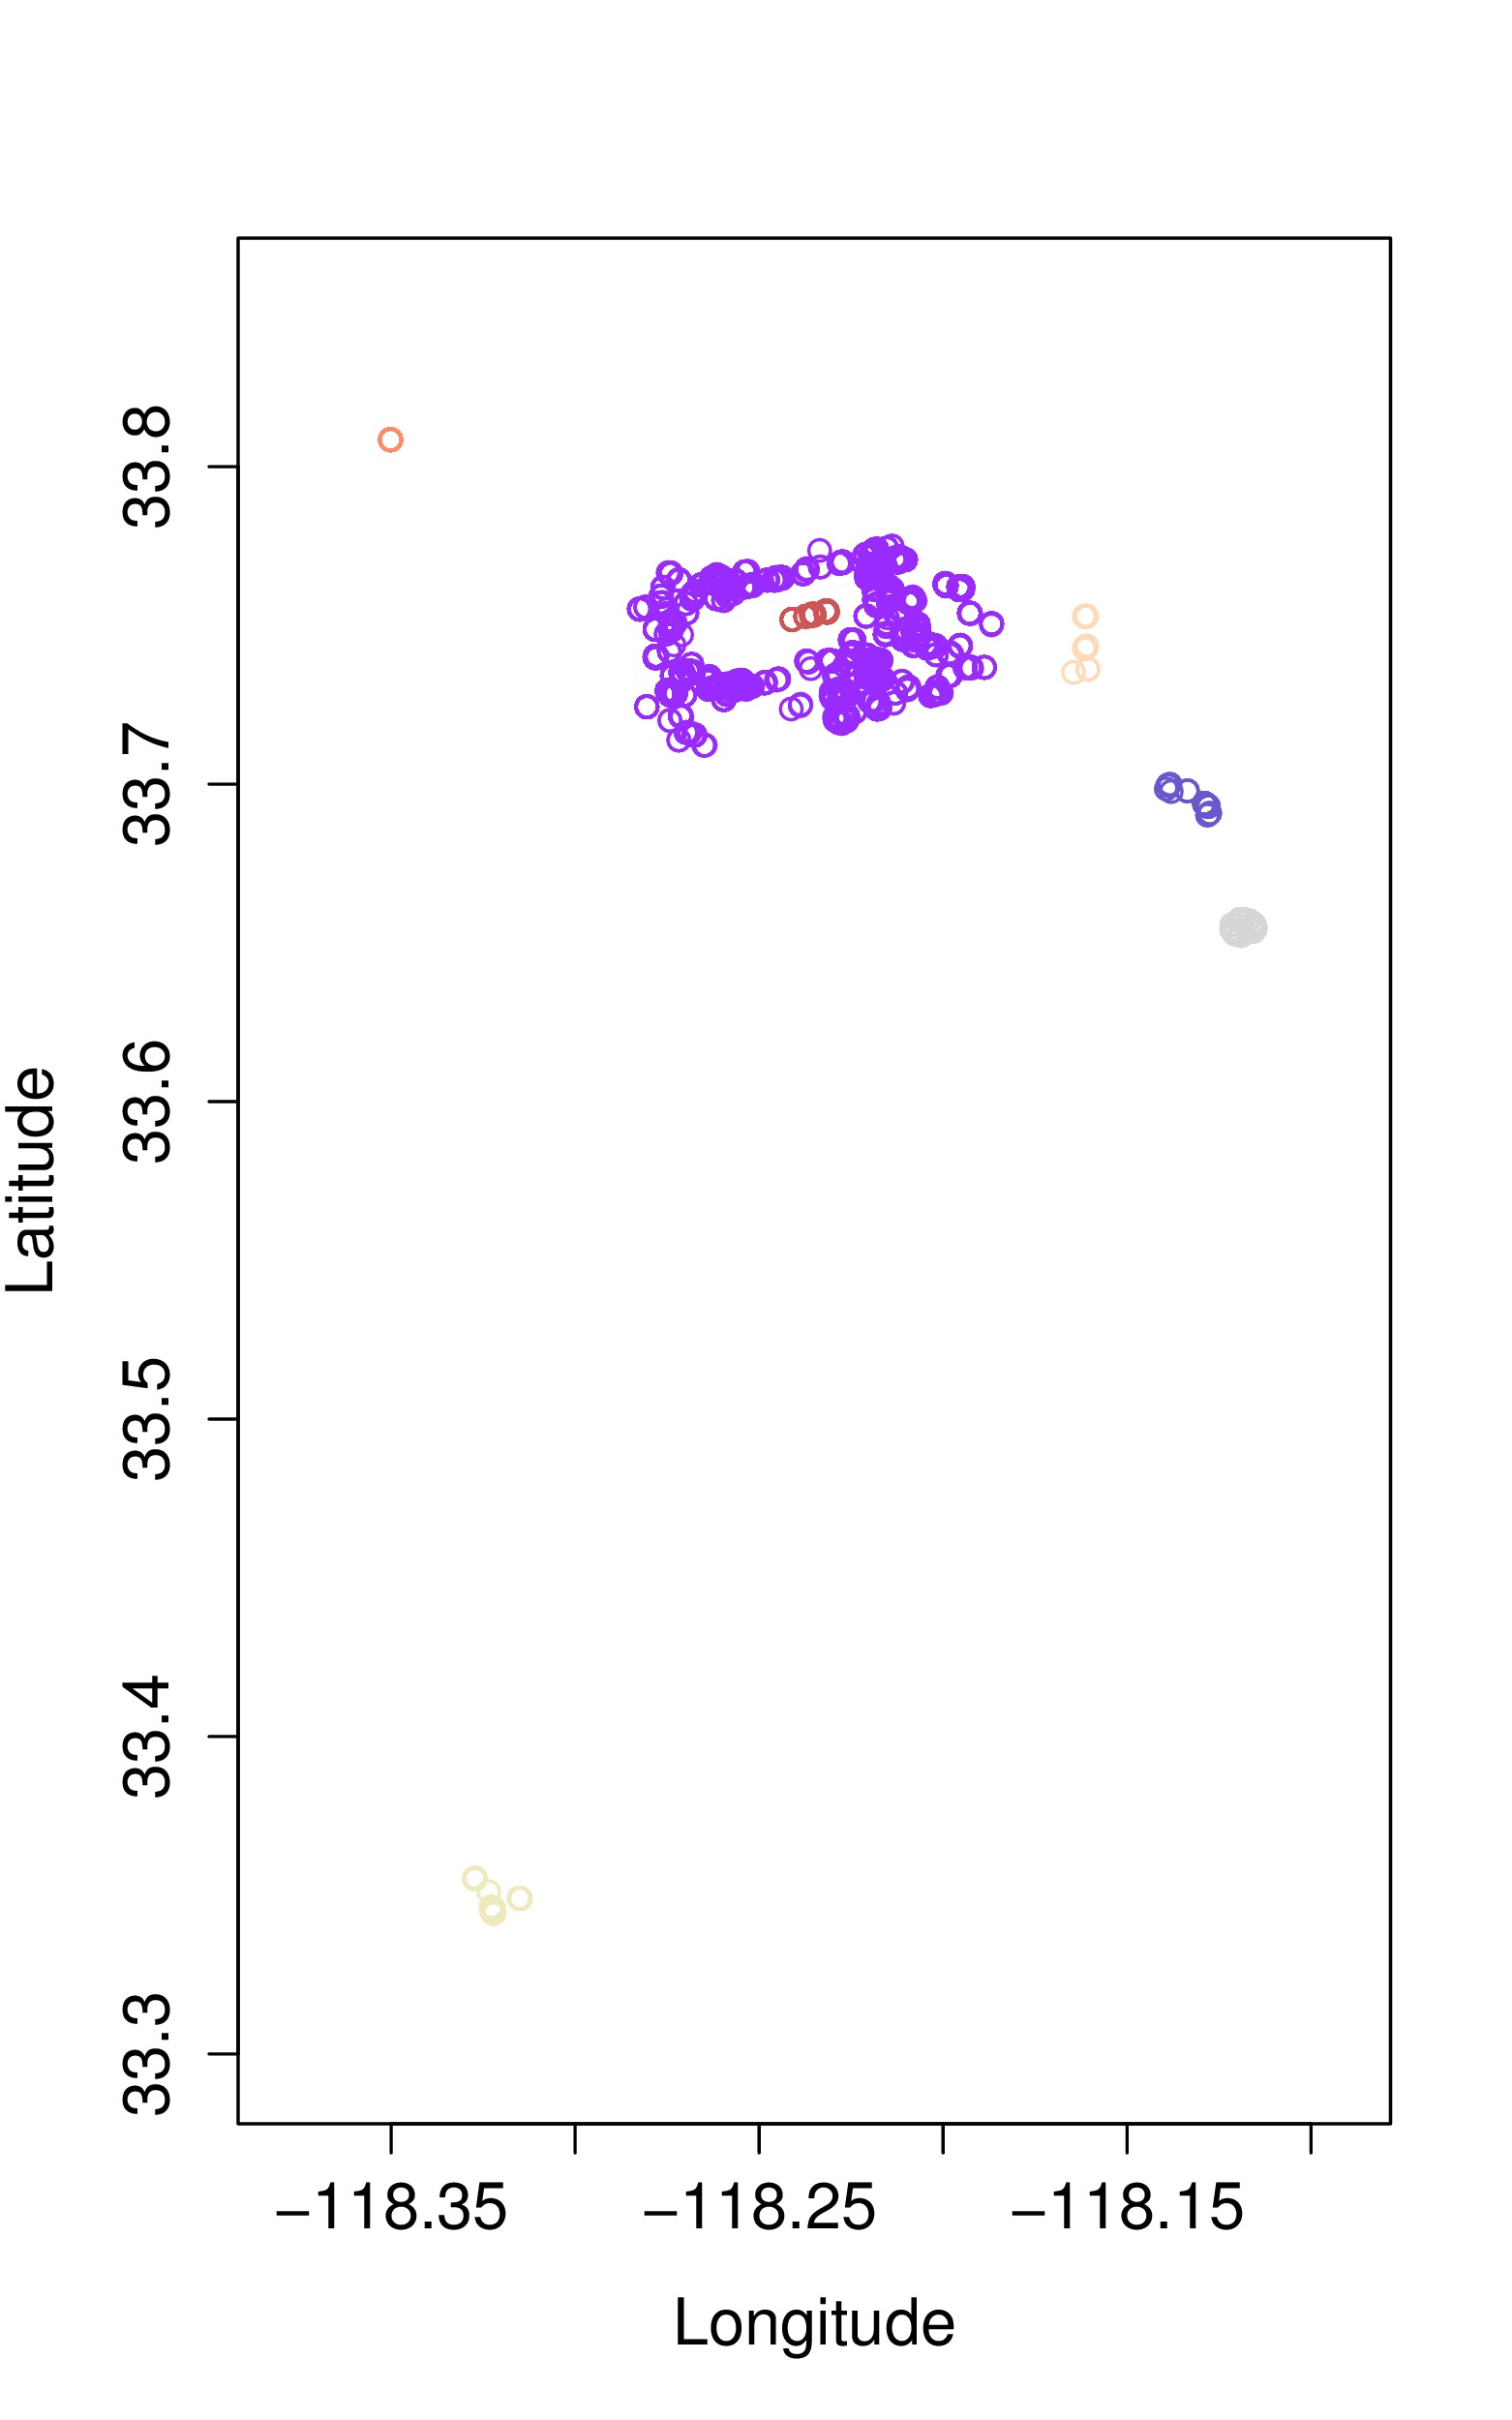
\includegraphics[width=2.66in]{LAStopOriginal.jpg}}
    \subfigure[Stopping clusters and Sampled Stopping Points generated]{\label{LAb}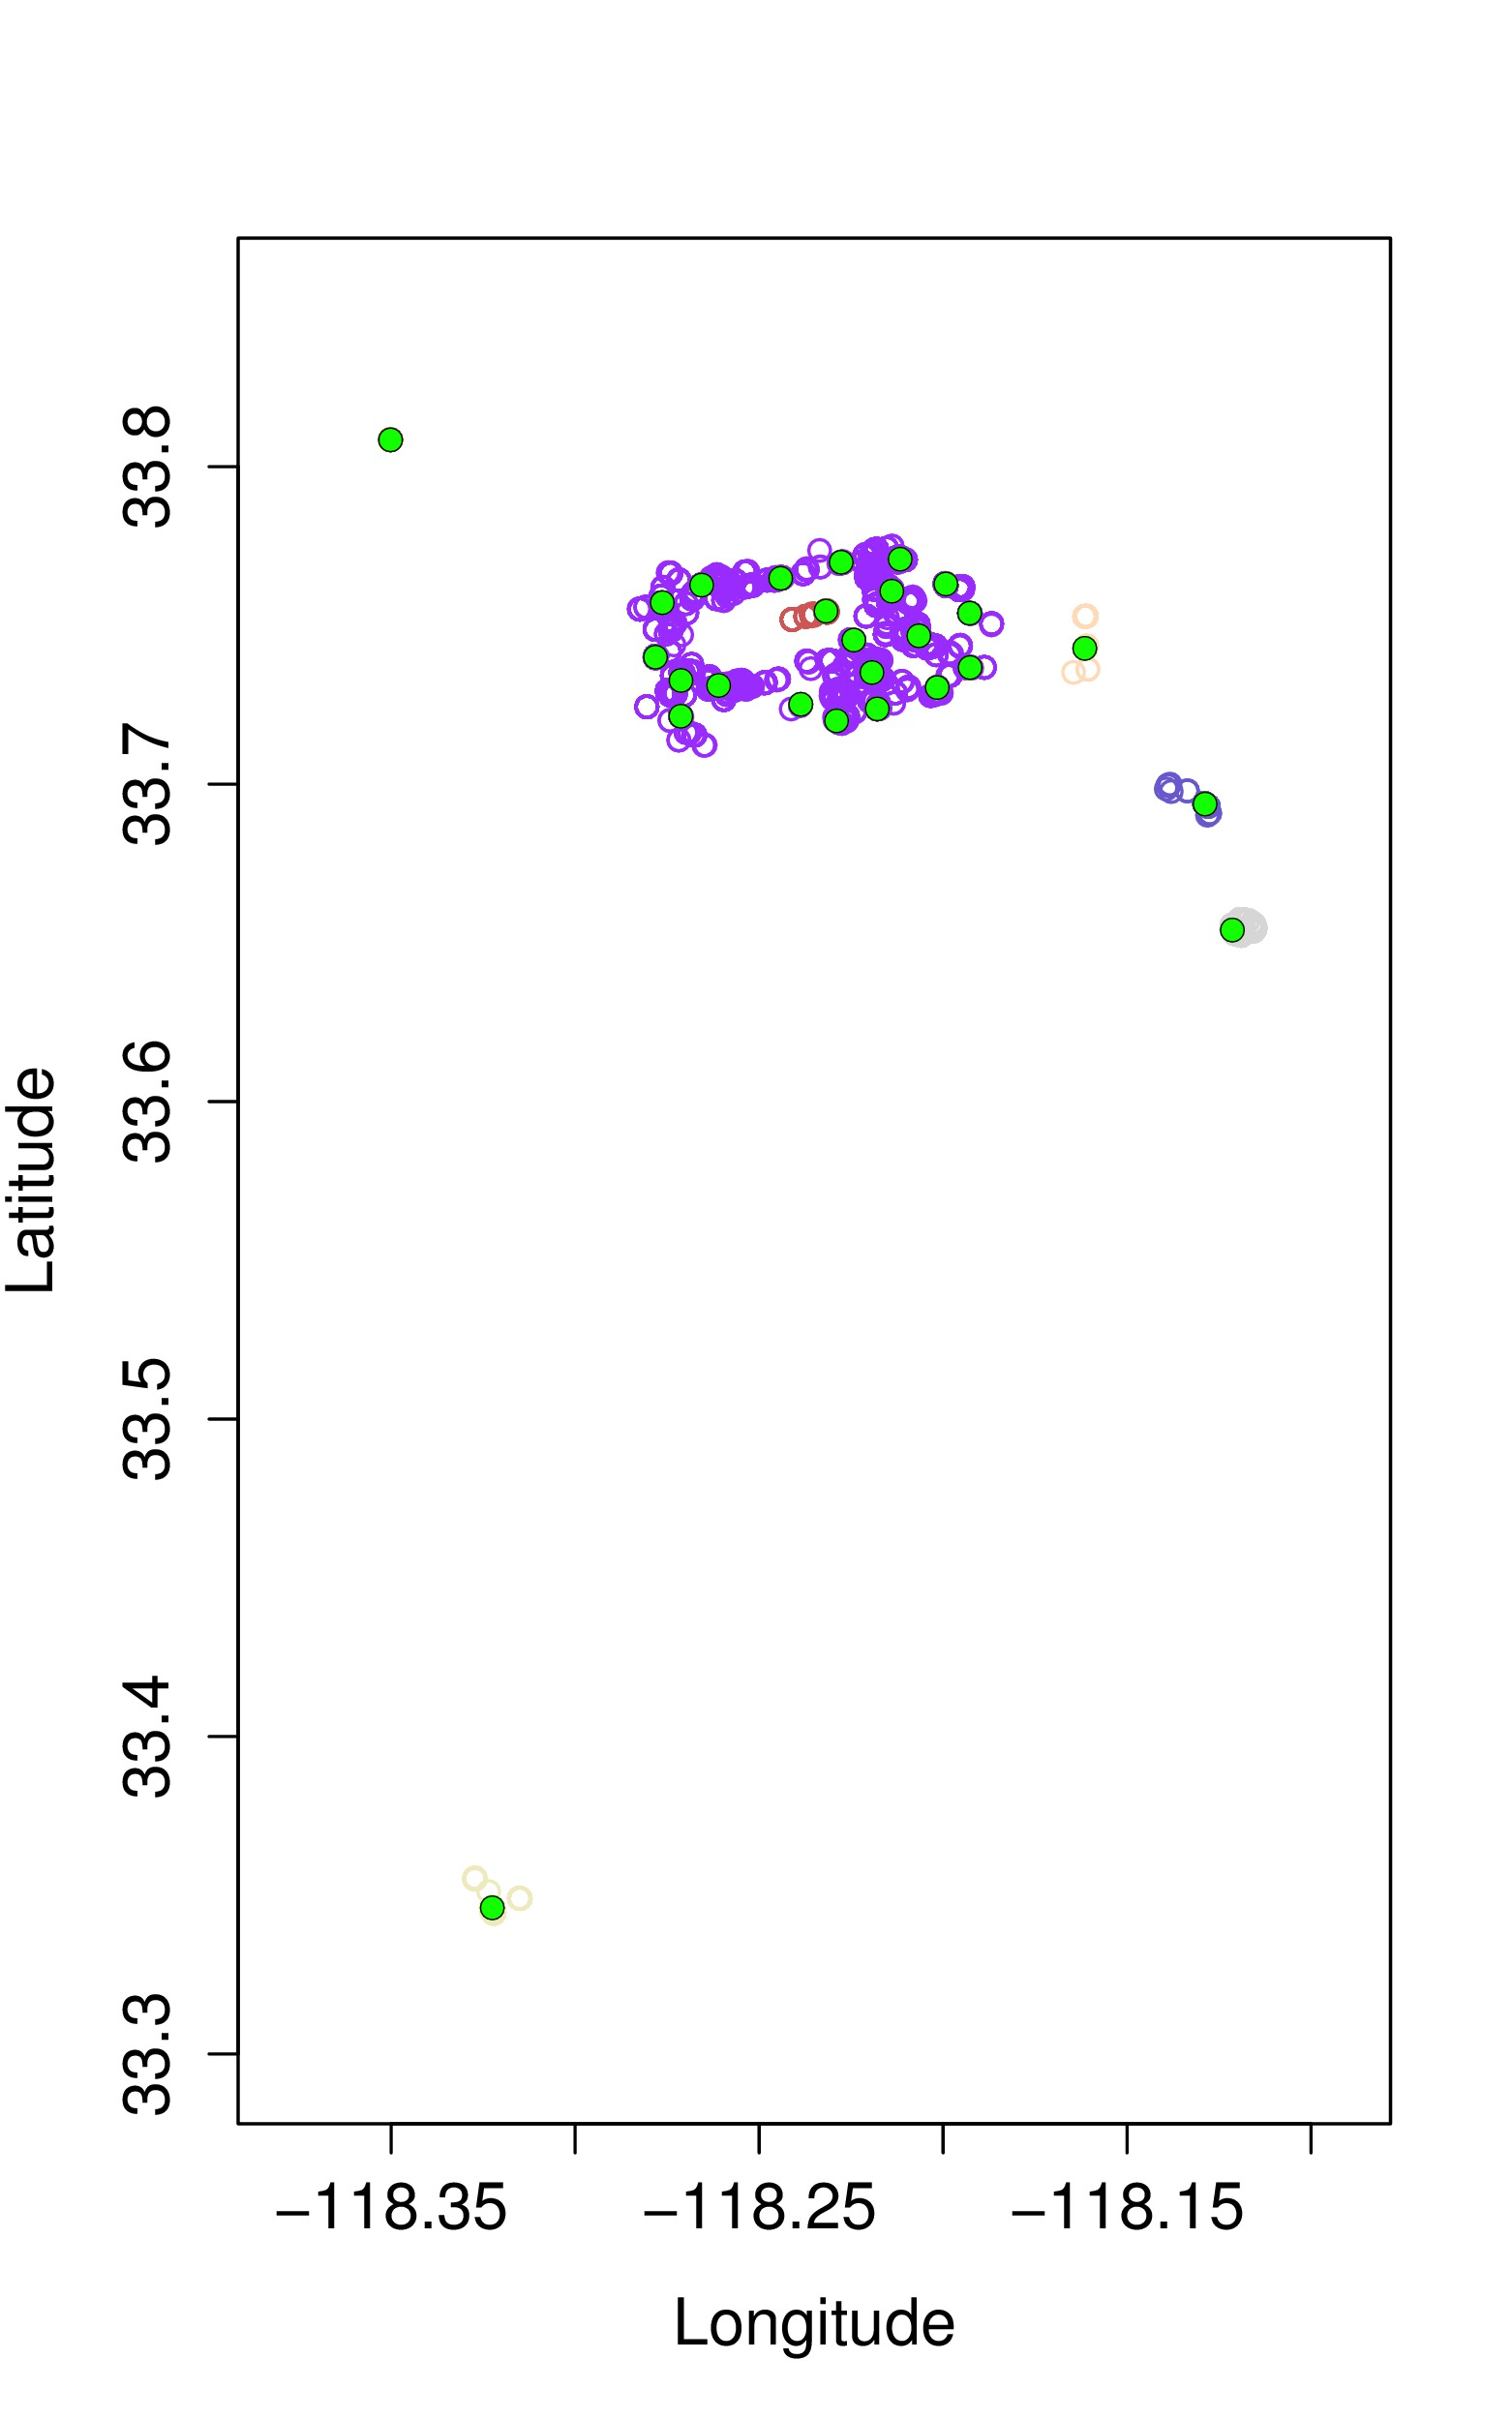
\includegraphics[width=2.66in]{LAnormalStop1.jpg}}
    \subfigure[Sampled Stopping Points generated]{\label{LAc}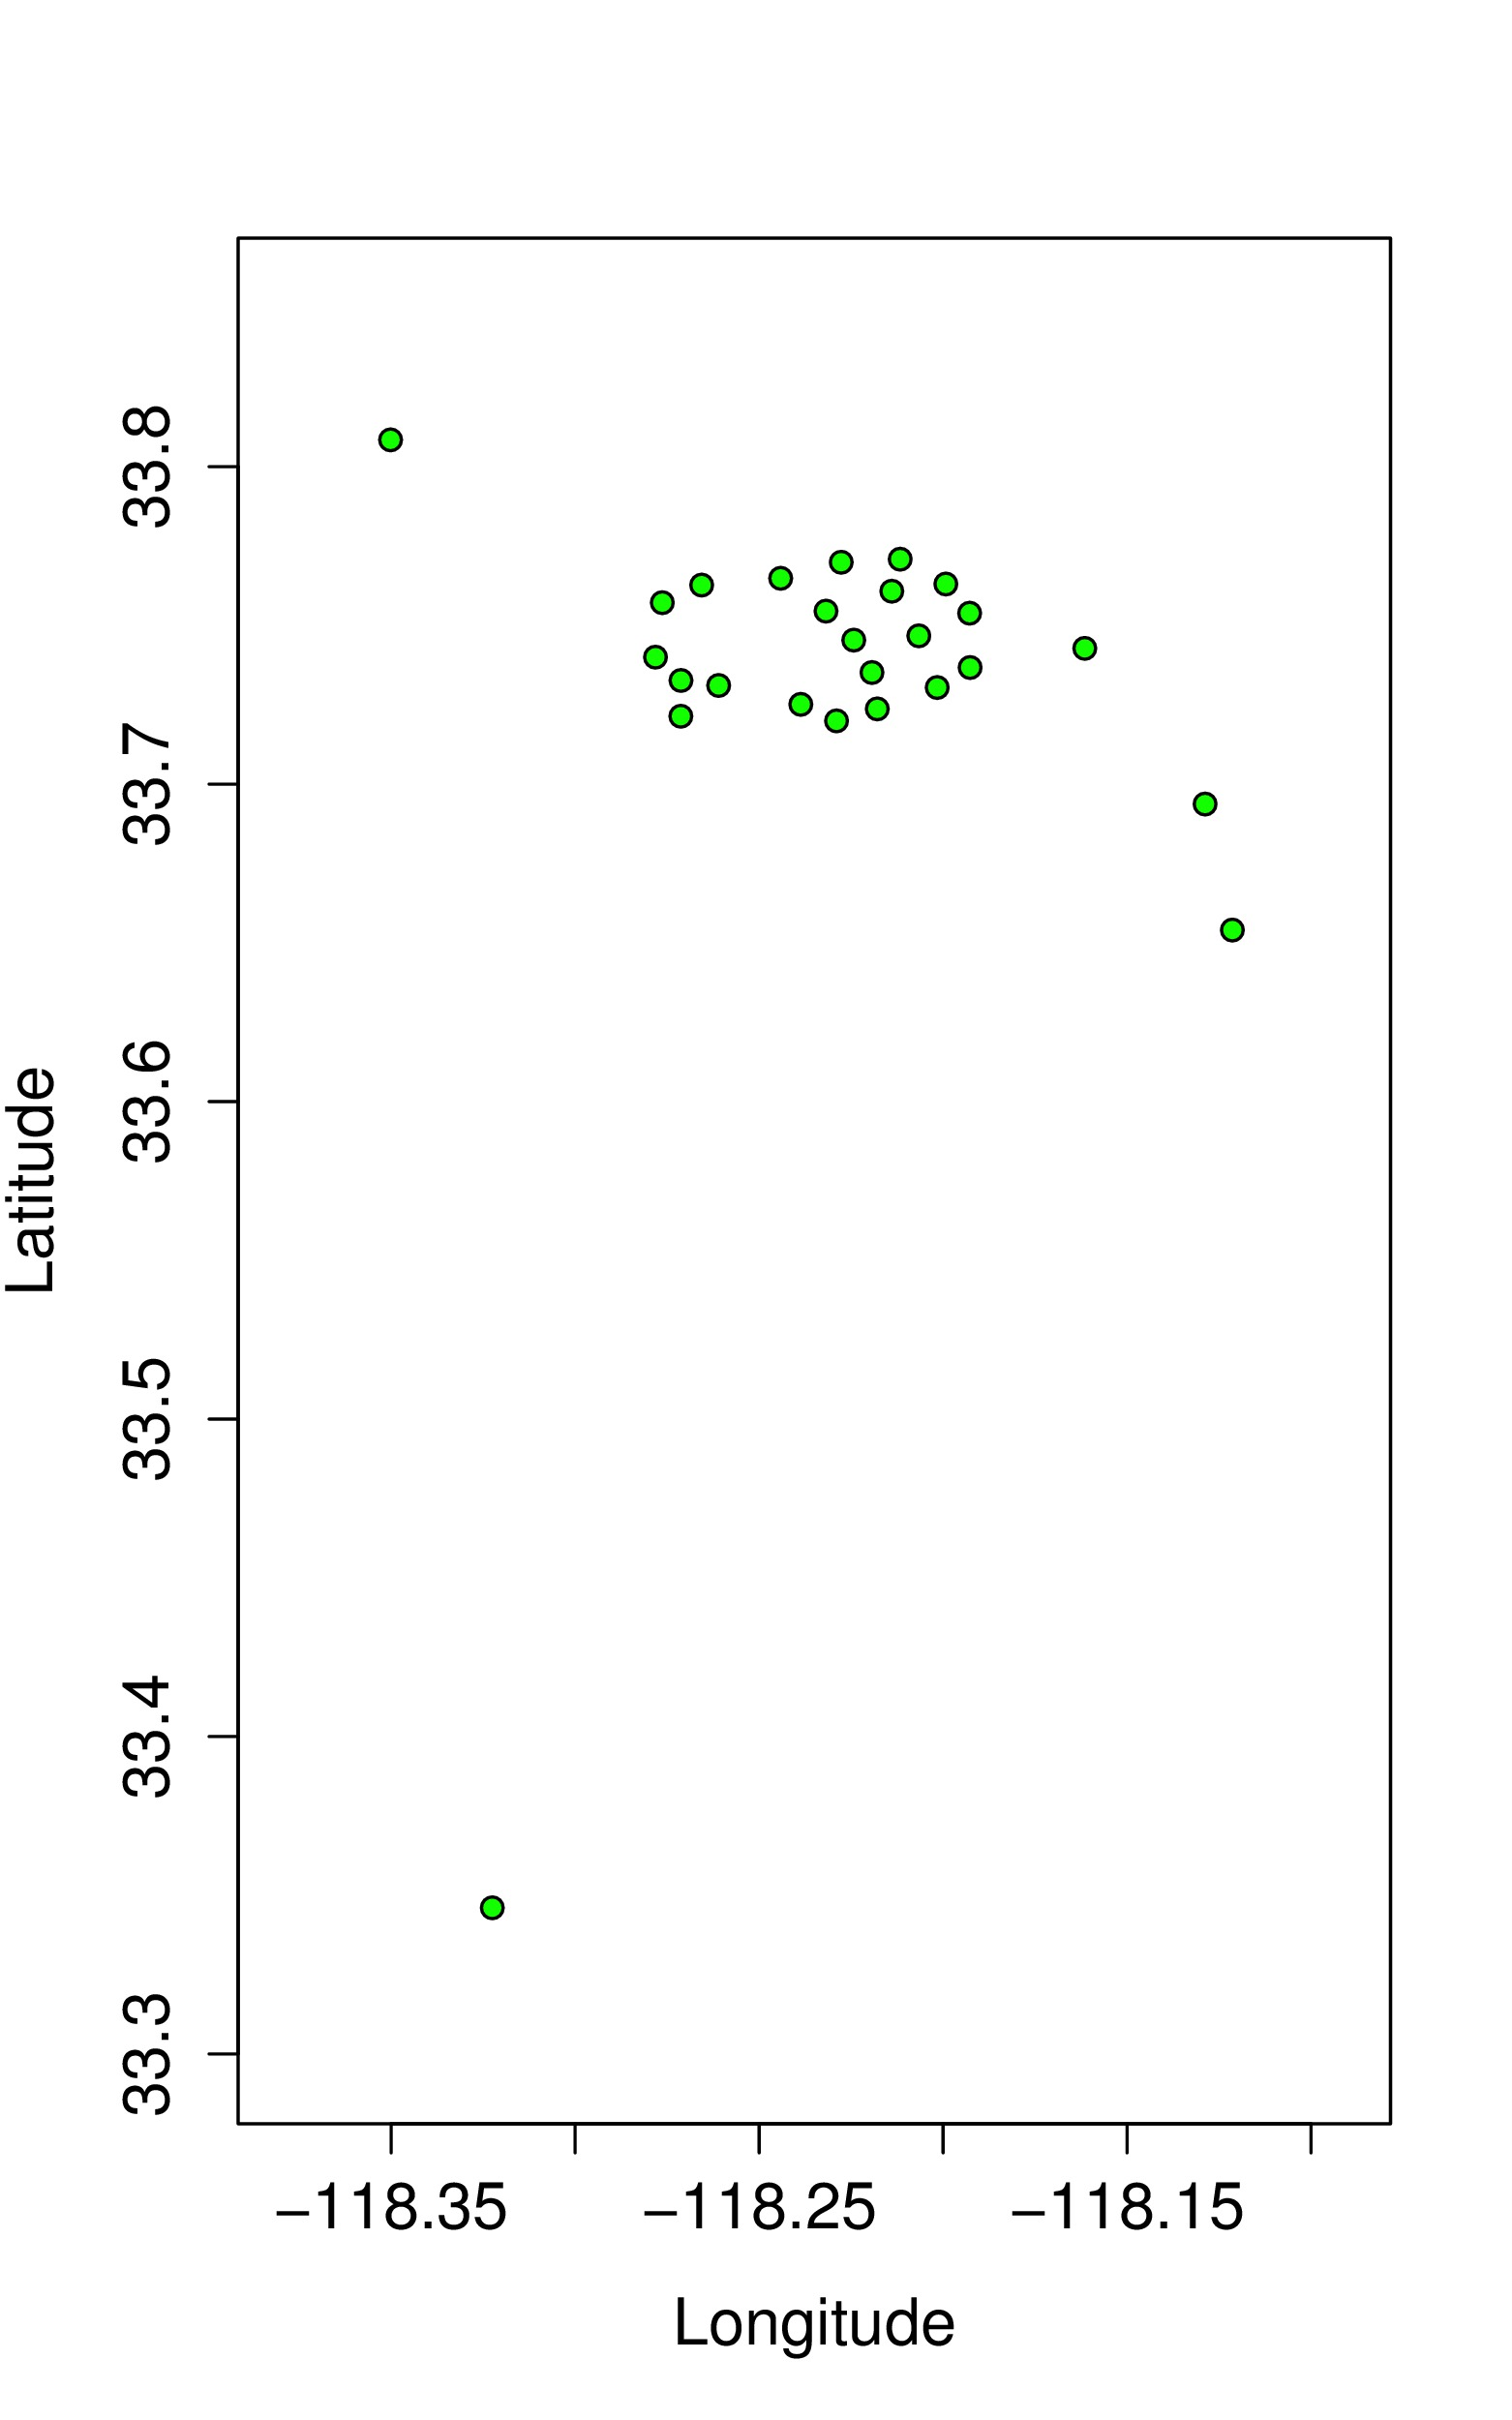
\includegraphics[width=2.66in]{LAnormalStop2.jpg}}
    \caption{Extract Stopping Sampling Points (SSP) from stopping clusters in Los Angeles Port Area. The stopping clusters are first extracted using DBSCAN \cite{DBScan96} algorithm shown in (a) and different colors stand for different clusters. Then Algorithm \ref{algo2} is used for getting the SSPs (shown in figures (b) and (c))}
    \label{LA}
\end{sidewaysfigure}


% \begin{figure*}[!htb]
% \centering     %%% not \center
% \subfigure[Stopping clusters by DBSCAN \cite{DBScan96} ]{\label{LAa}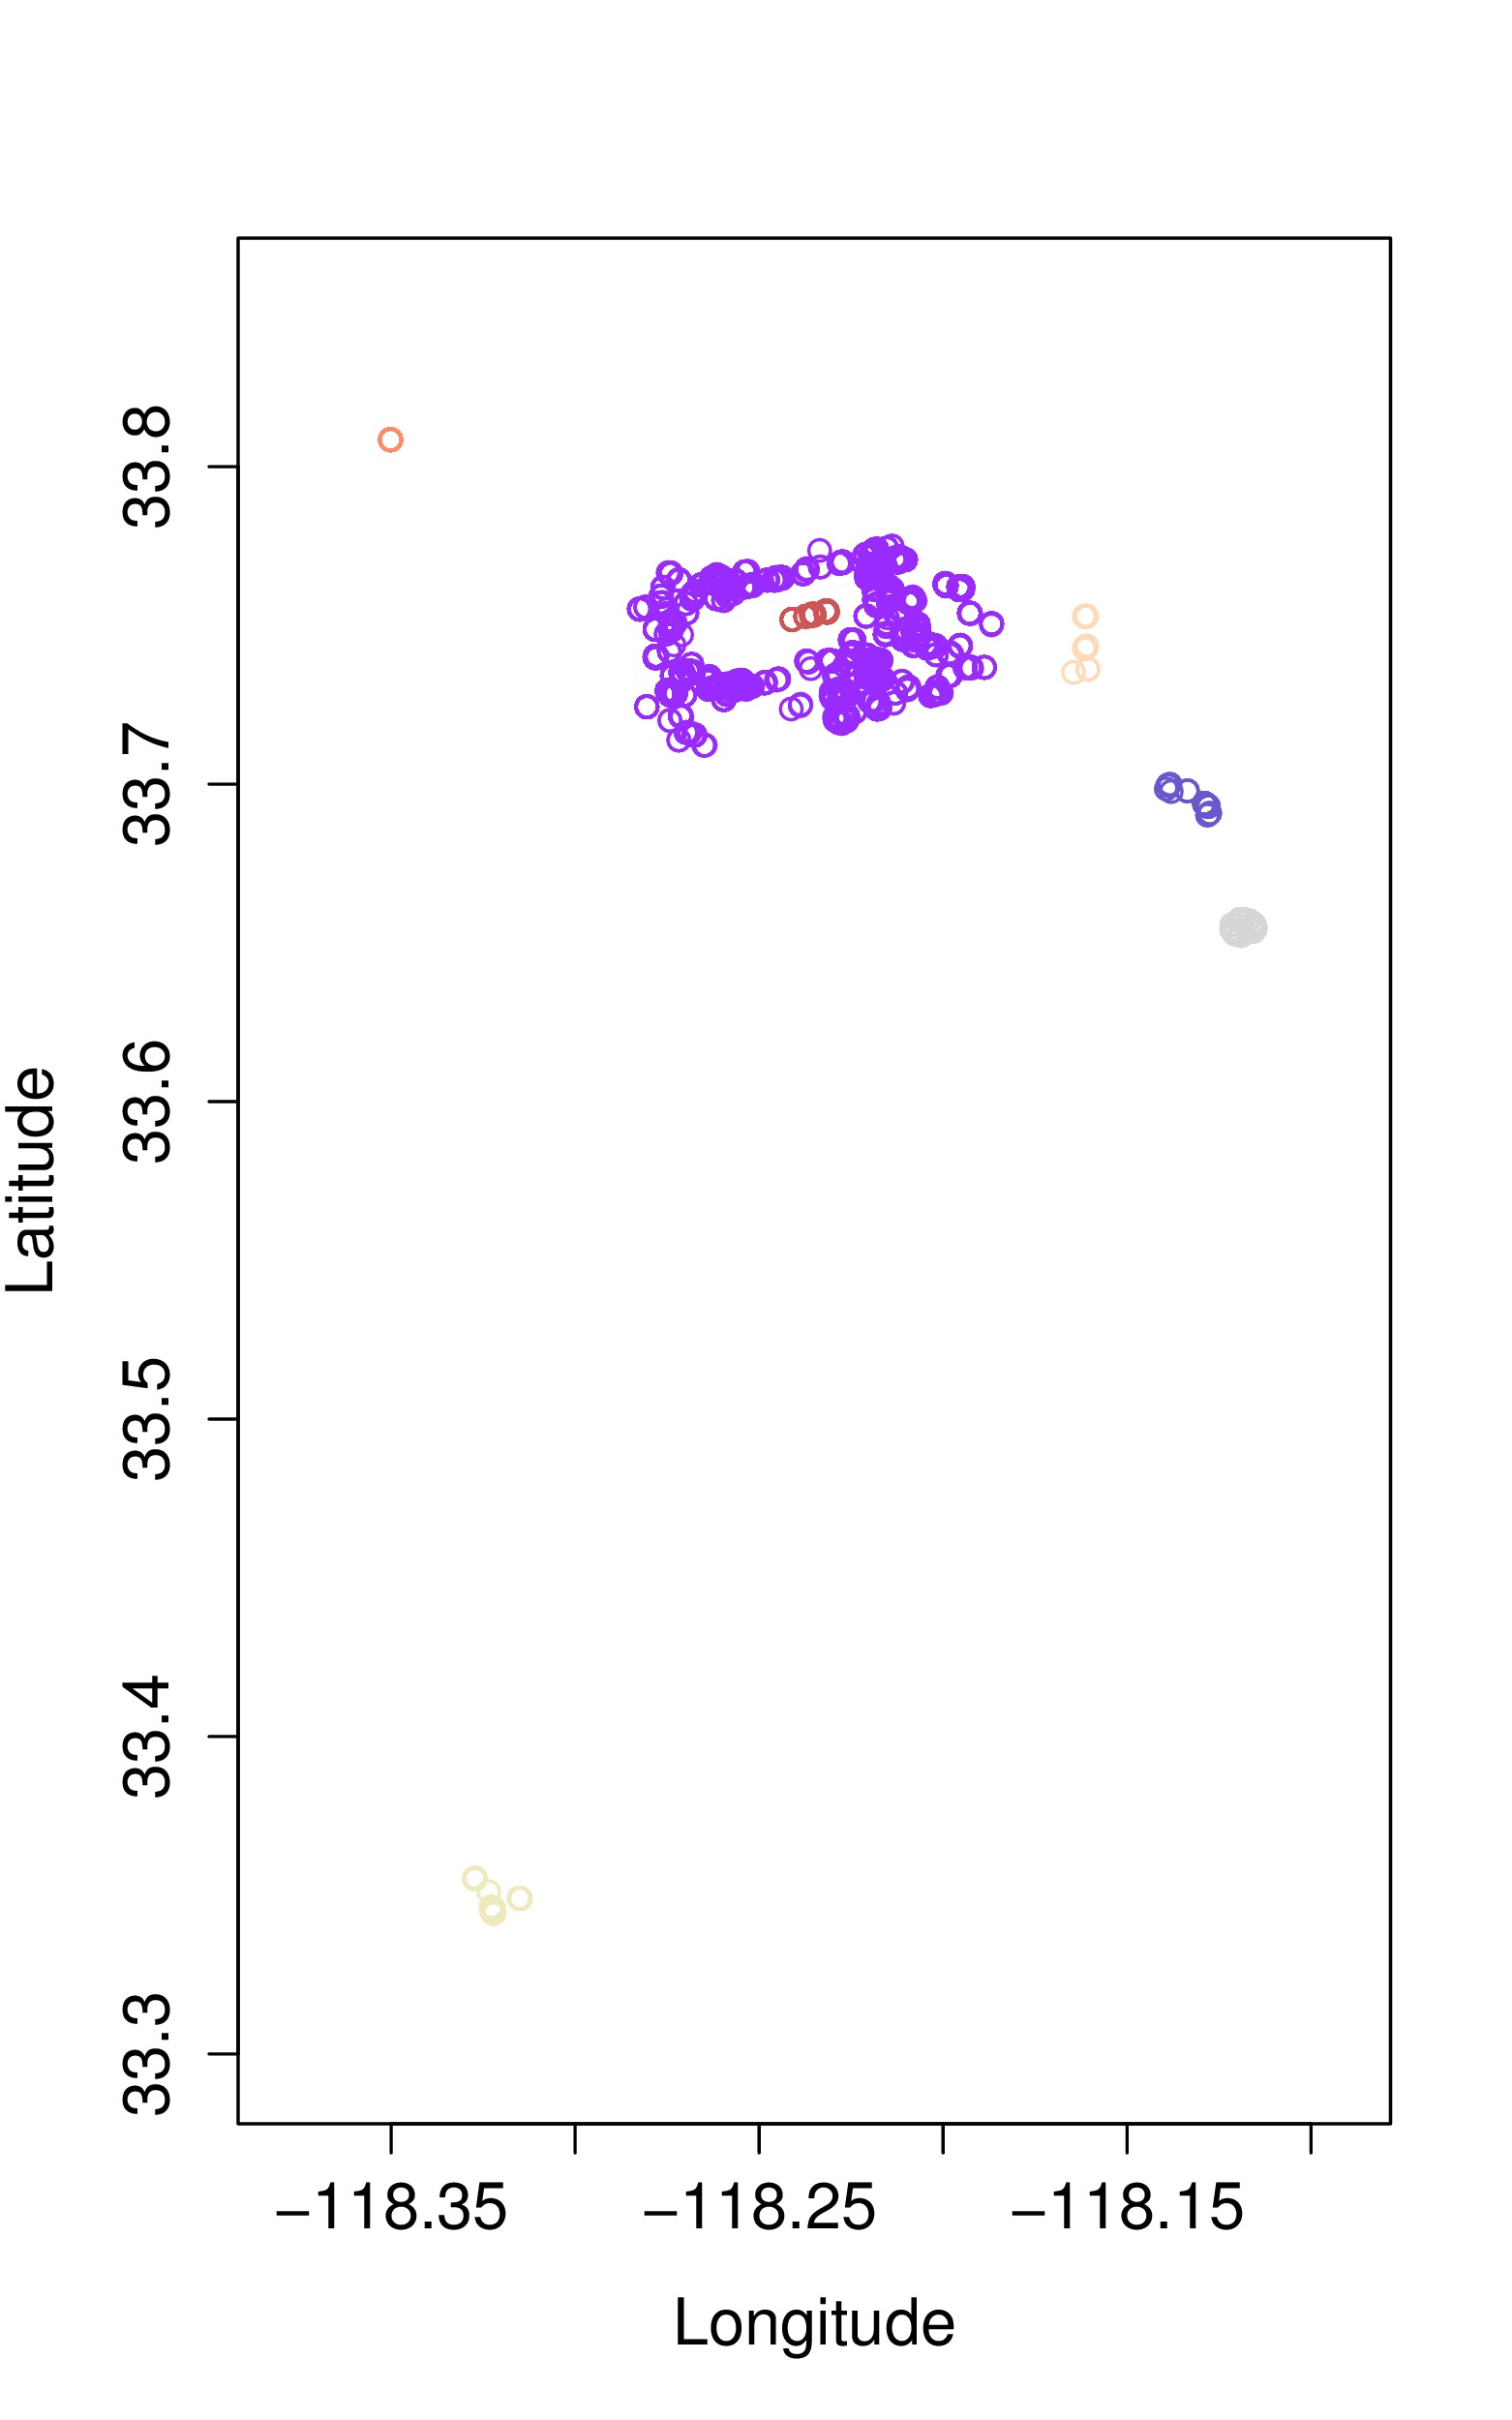
\includegraphics[width=1.95in]{LAStopOriginal}}
% \subfigure[Sampled Stopping Points generating]{\label{LAb}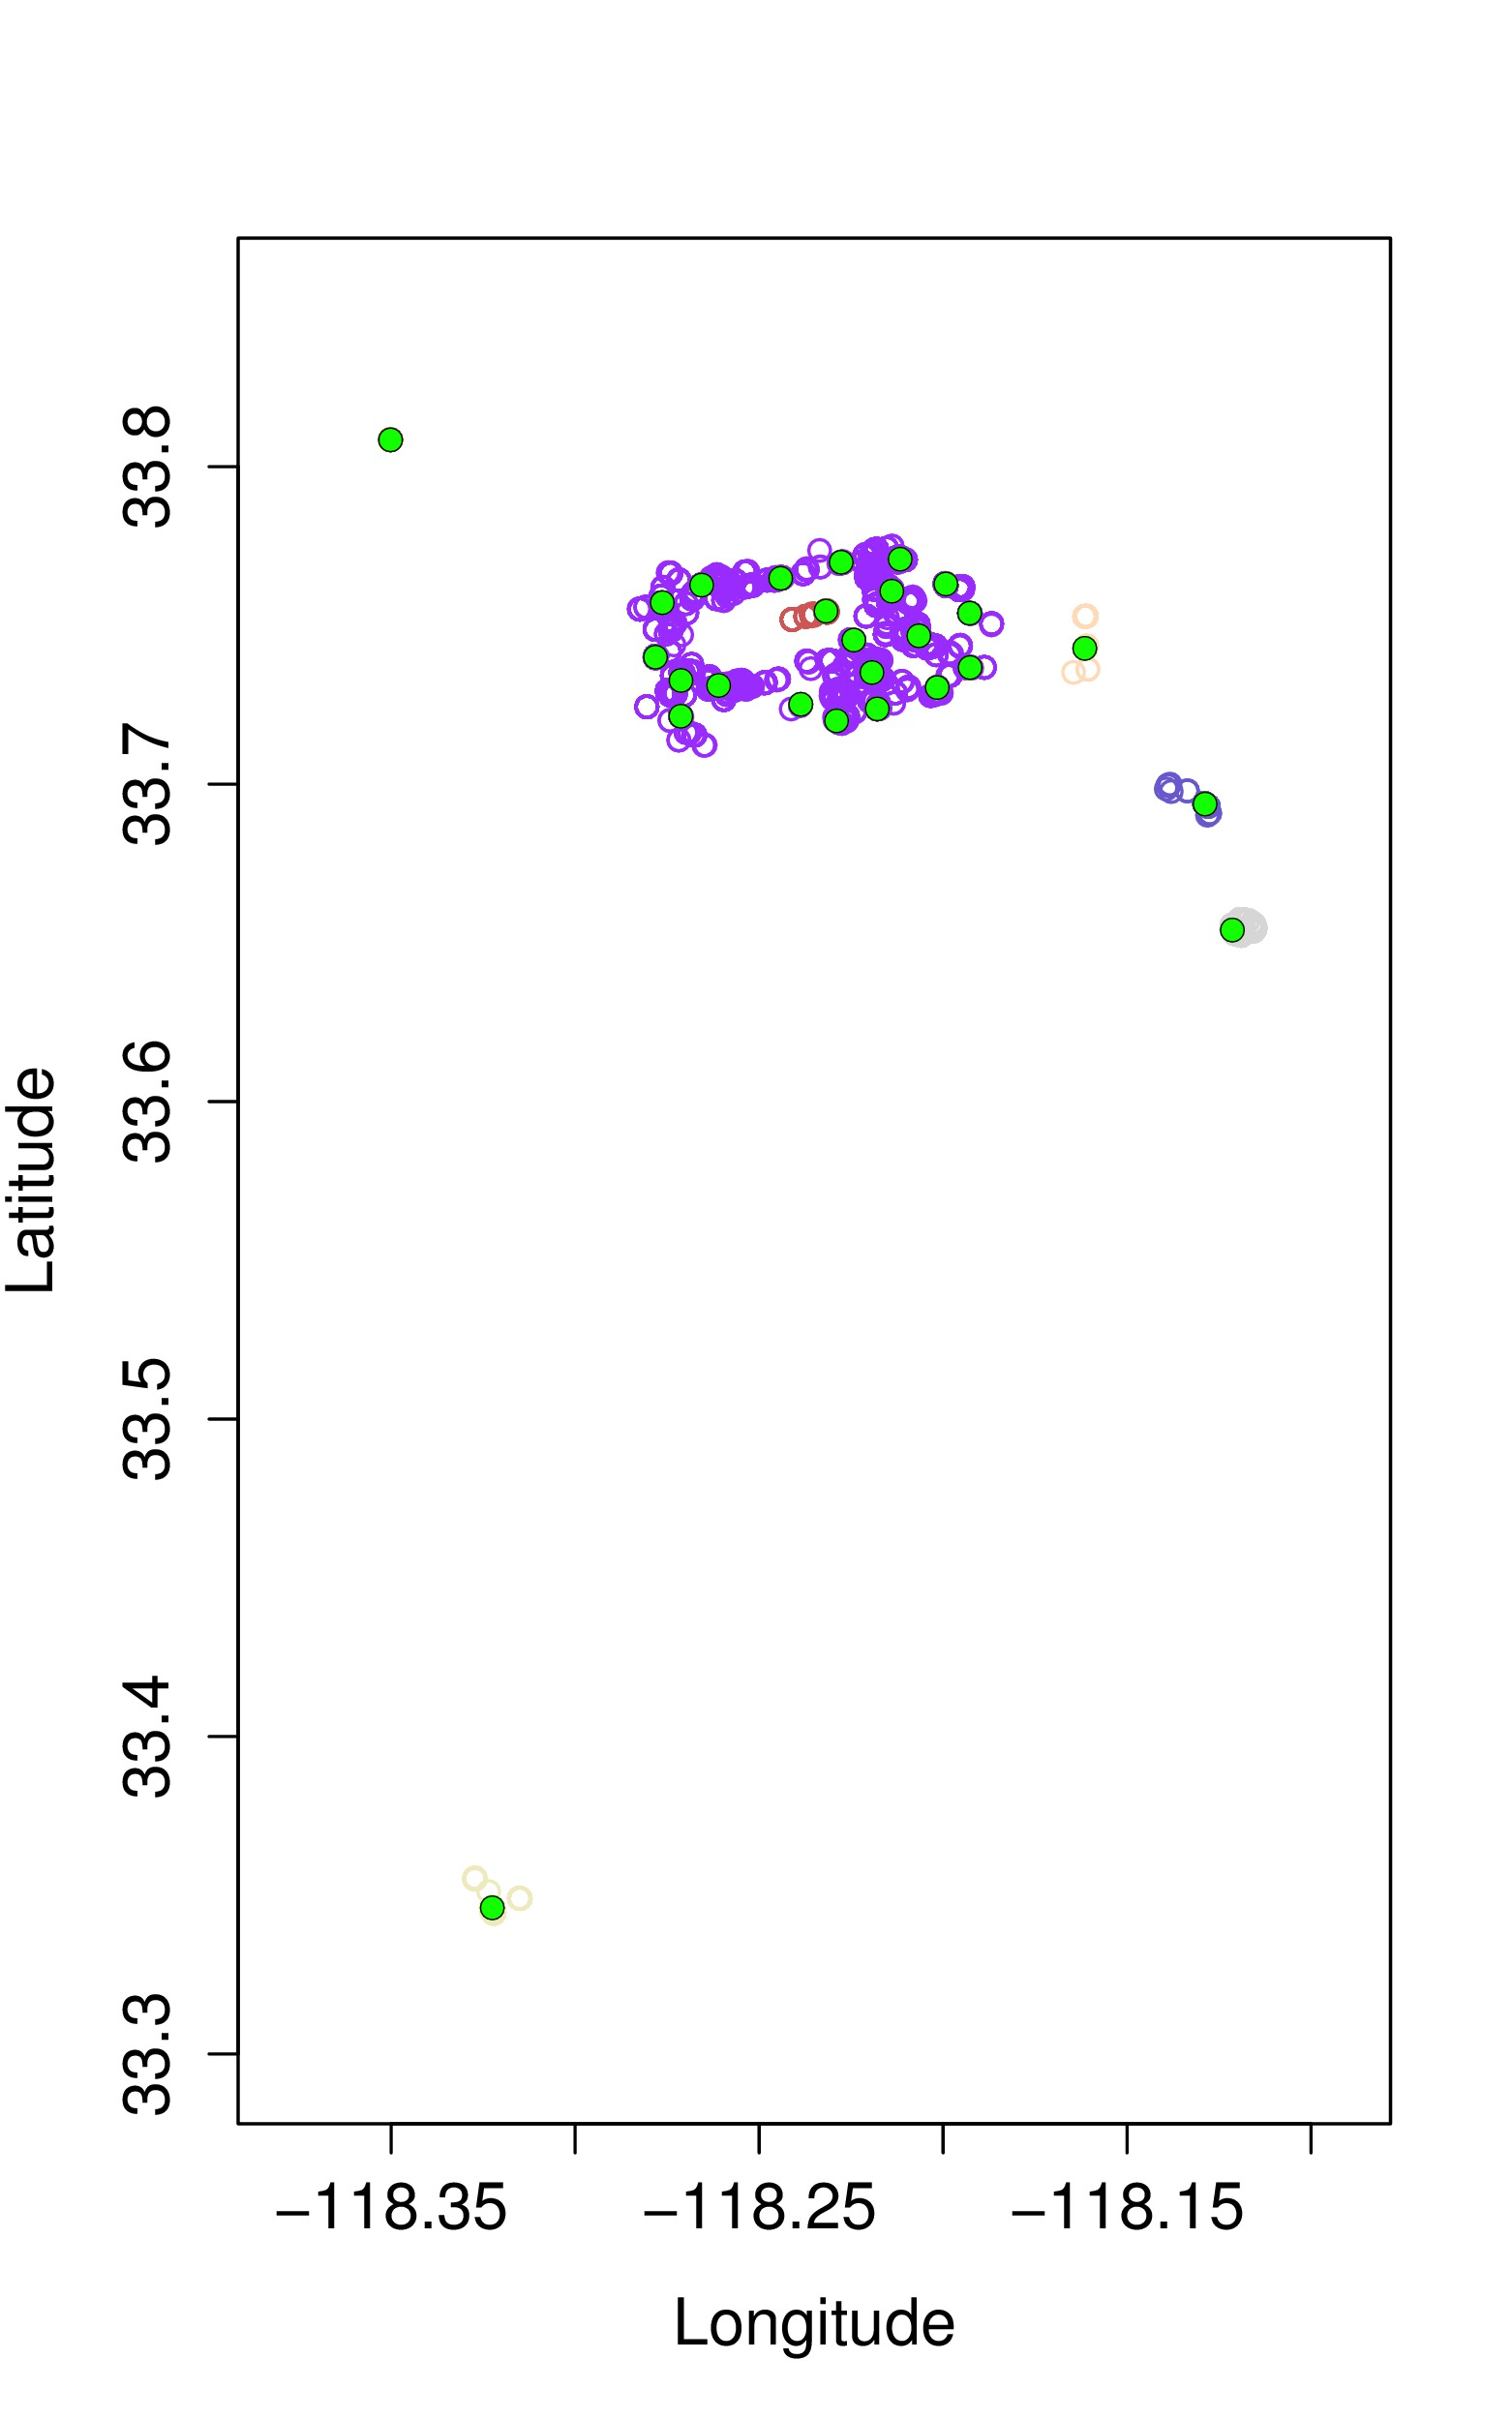
\includegraphics[width=1.95in]{LAnormalStop1}}
% \subfigure[Sampled Stopping Points generated]{\label{LAc}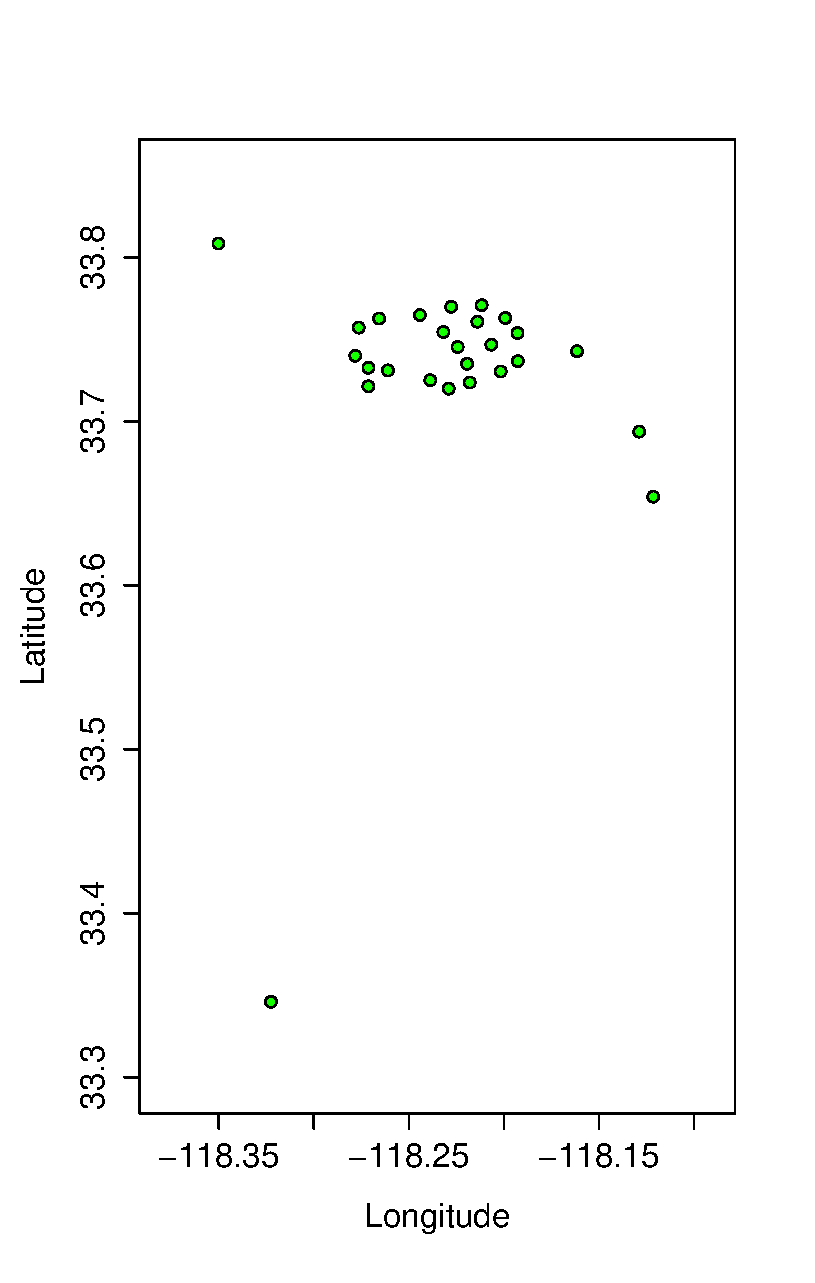
\includegraphics[width=1.95in]{LAnormalStop2}}
% \caption{Extract Stopping Sampling Points (SSP) from stopping clusters in Los Angeles Port Area. The stopping clusters are first extracted using DBSCAN \cite{DBScan96} algorithm shown in (a) and different colors stand for different clusters. Then Algorithm \ref{algo2} is used for getting the SSPs (shown in figures (b) and (c))}
% \label{LA}
% \end{figure*}



Figure \ref{LA} shows the result of stopping clusters sampling procedure in the area of Los Angeles Long Beach. There are 7 different stopping clusters in Figure \ref{LAa} with 19,089 stopping points generated by DBSCAN algorithm \cite{DBScan96}. Then after applying Algorithm \ref{algo2}, only 26  Stopping Sampled Points (shown in green color in Figure \ref{LAb} and \ref{LAc}) are selected with excellent quality in terms of the representativeness.

\begin{figure}[!htb]
\centering
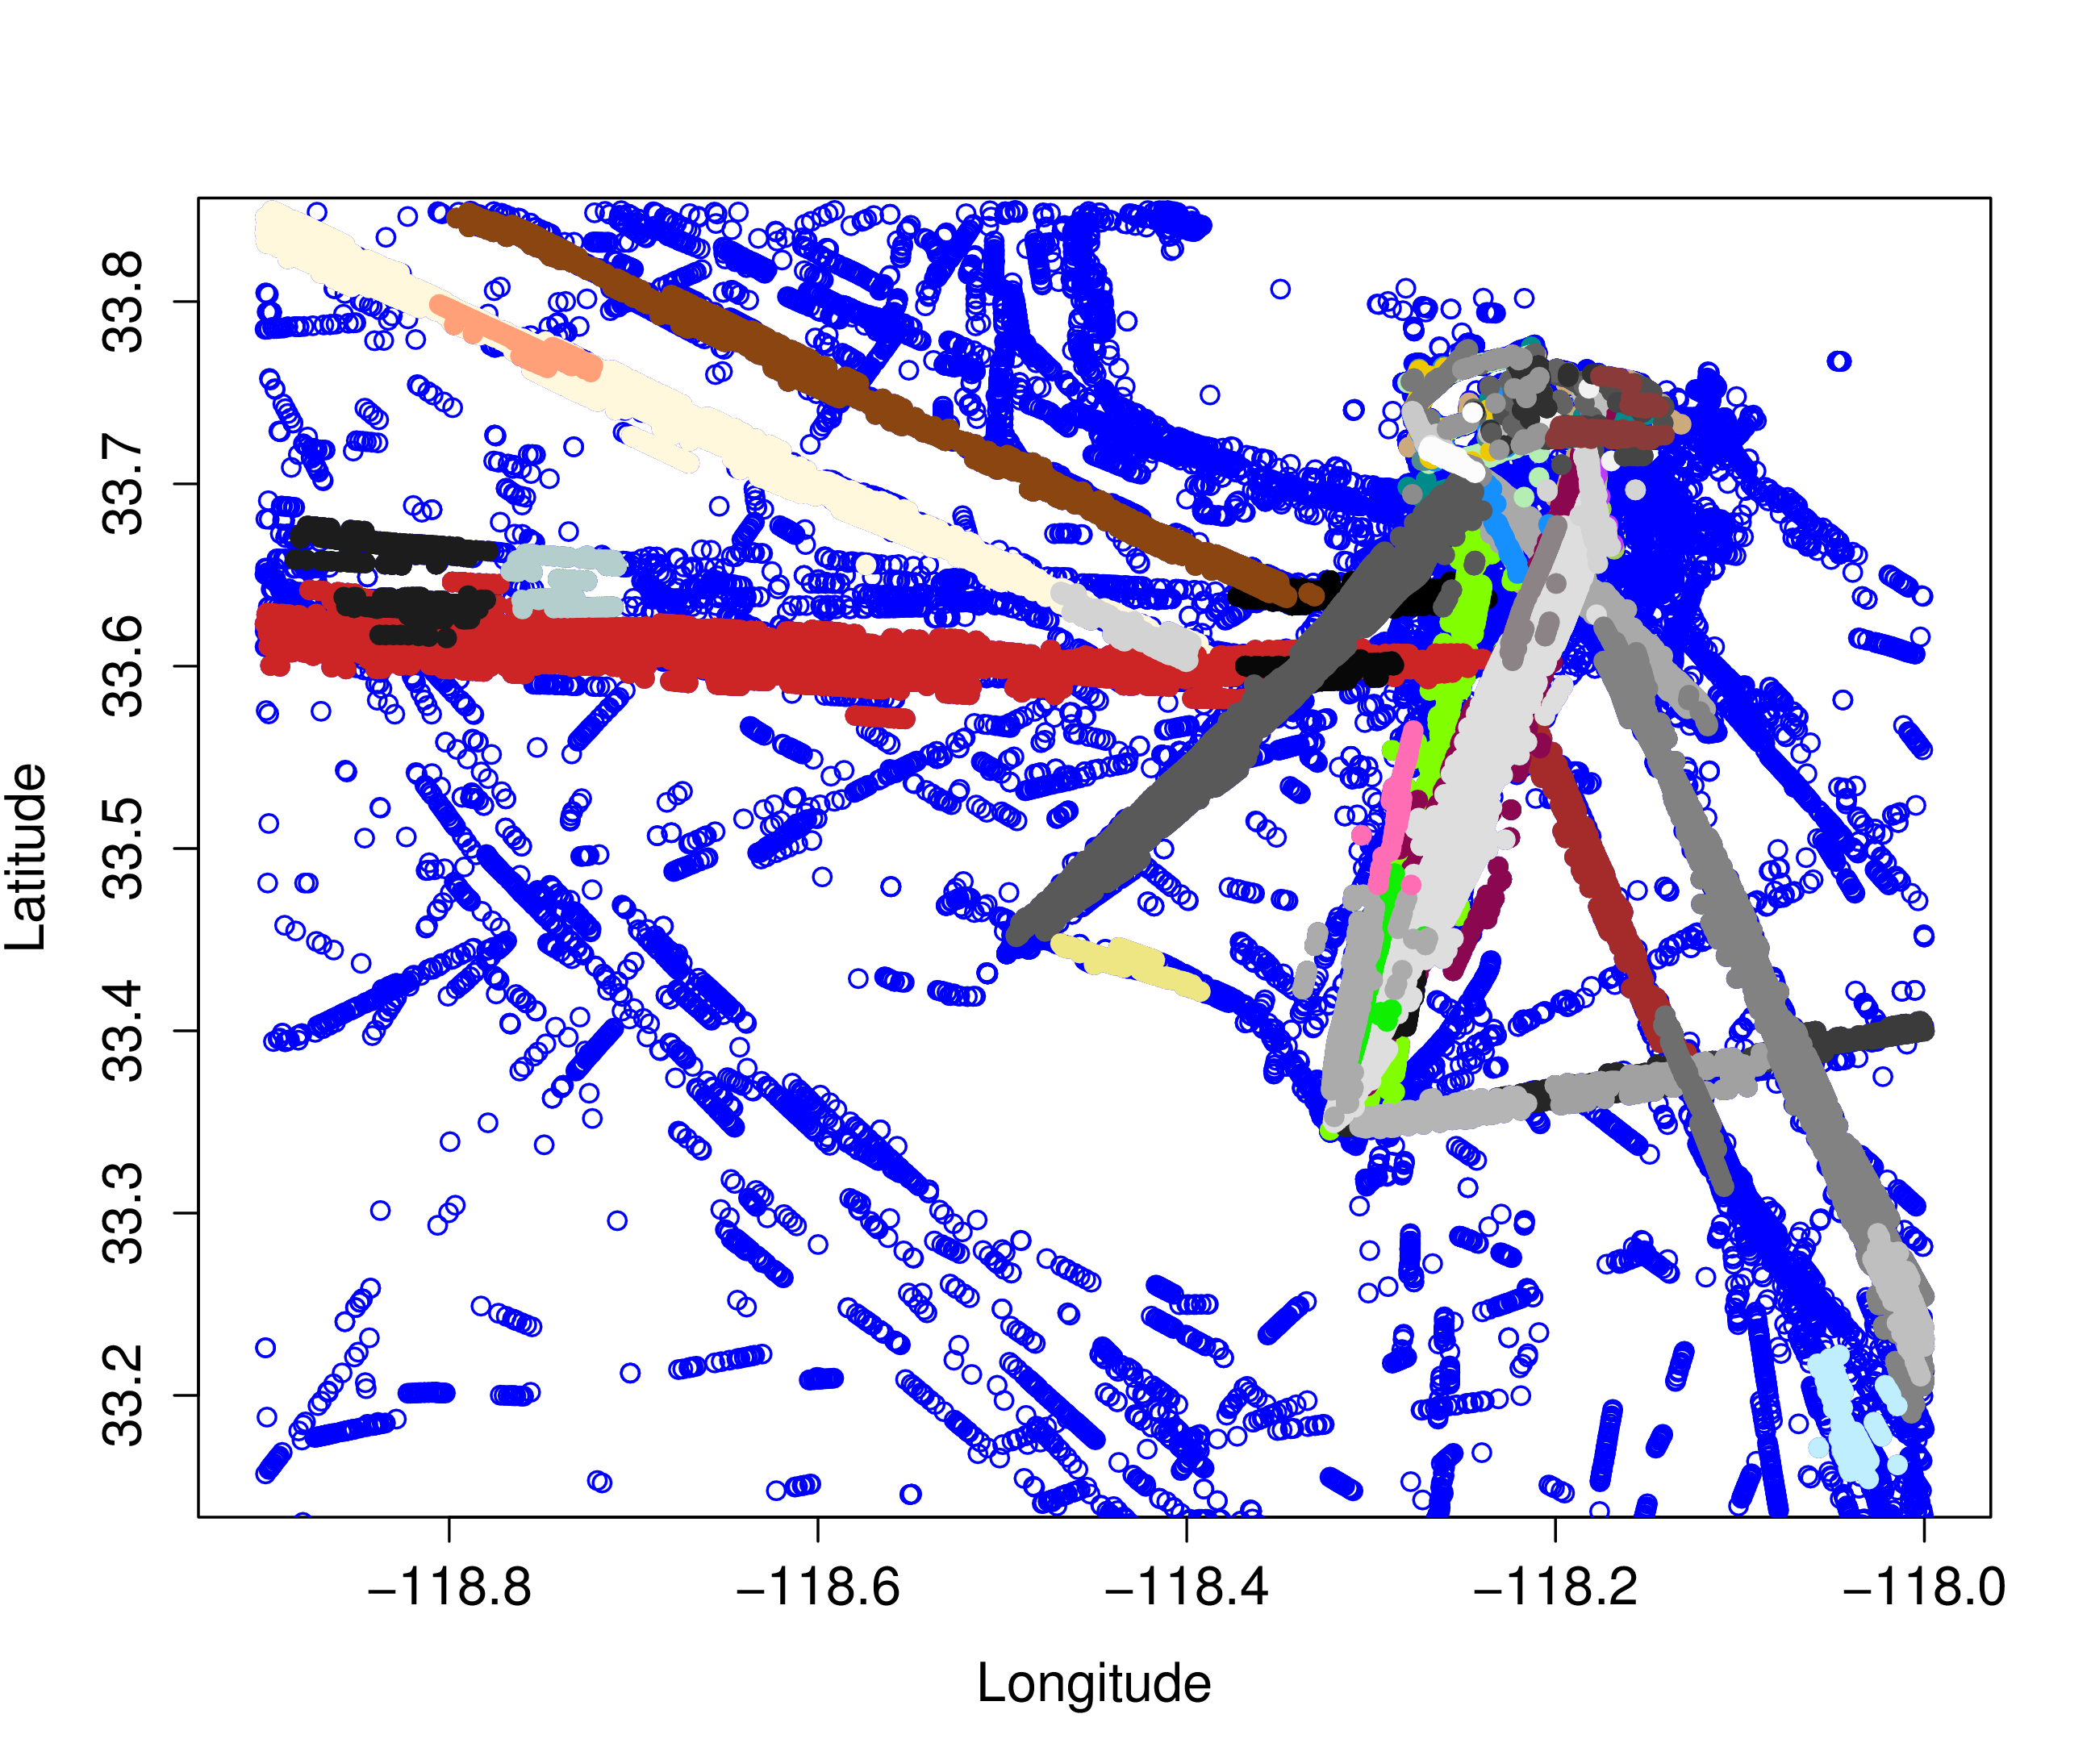
\includegraphics[width=5in]{LAmoveOrig.png}
\caption{The clustering results of Los Angeles Long Beach area. This only shows the moving points(in blue) and the corresponding moving clusters (in different colors).}
\label{fig:la_movecluster}
\end{figure}

\begin{figure}[!htb]
\centering
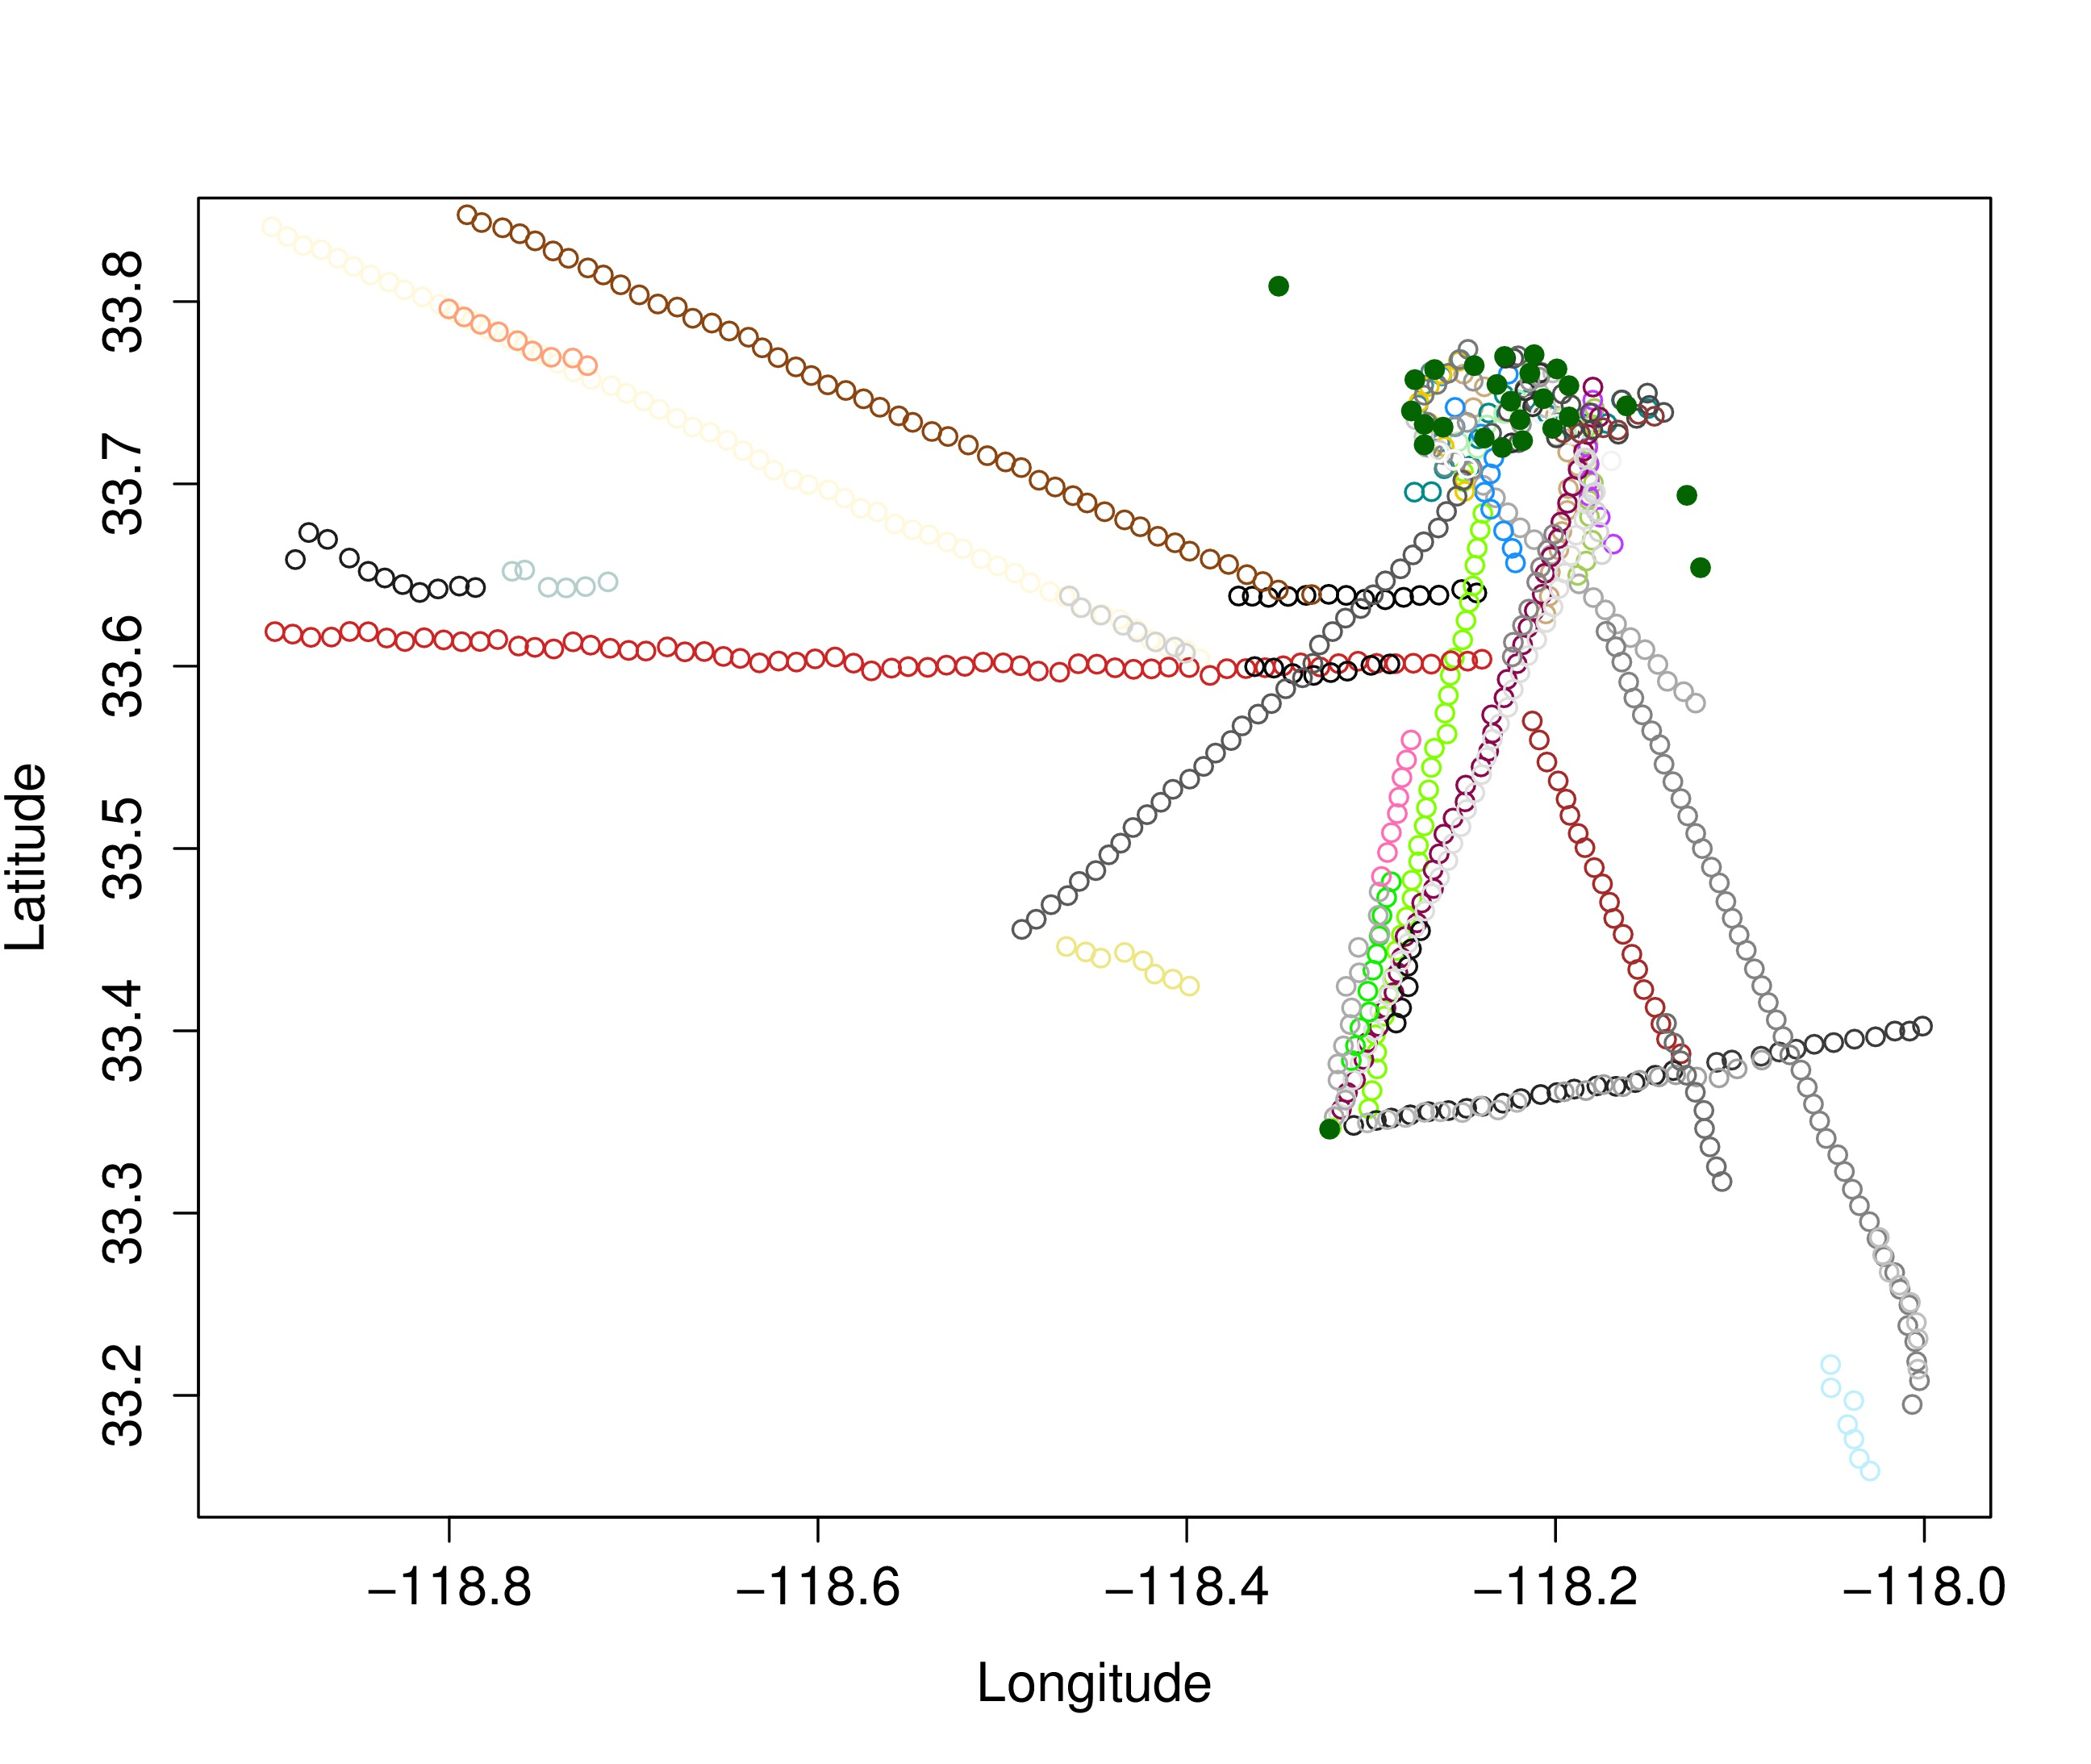
\includegraphics[width=5in]{LAclustersGV.jpg}
\caption{The Gravity Vectors and Sampled Stopping Points extracted from the clusters in Los Angeles Long Beach area. }
\label{fig:la_clusters}
\end{figure}

Then the algorithm DBSCANSD is applied to moving points. Ultimately, 48,404 points are selected to form 51 moving clusters from the original 99,937 points. This result is shown in Figure \ref{fig:la_movecluster}. From the figure we can see that in the stopping area, there are multiple moving clusters too. This is because vessels in the area have to change their headings frequently to arrive at the specified anchor location and our algorithm will treat this curve-shape movement as multiple moving clusters with slight COG differences. The last step for this normal traffic pattern extraction is to calculate the Gravity Vectors of the moving clusters. The GVs of the area can be seen in Figure \ref{fig:la_clusters} and the SSPs (filled circles in dark green color) extracted in the previous step are also shown in the same figure.


\section{Anomaly Detection Model}
\label{sec:exp_2}
In this section, we evaluate the effectiveness of our maritime anomaly detection model in the region of Juan de Fuca Strait. %The data set belongs to a private company and it contains information that may identify individuals, therefore this data is not public. 
The evaluation work contains two parts, the first one is conducted with the non-labeled data while the second one is done after labelling the data. The results of the first experiment are shown visually and the second experiment compares our model's results with the labels by the expert.

%Since our model is an unsupervised-based model, it is necessary to have the first type of experiment to show the effectiveness from a visualization way. Furthermore, the second one can compare our model's results with the labels by the expert.

The data set which was prepared for normal traffic patterns extraction phase comprises two months of trajectory data from November 1 to December 31 in 2012 and contains 67,850 trajectory points. The whole data set is not used for extracting normal patterns, instead 46,000 records (40,000 moving points and 6,000 stopping points distinguished by the SOG threshold 0.5 knots) are selected and then the rest of the data set is used for estimating the three thresholds for the anomaly detection phase. 

Afterwards, to evaluate our anomaly detection model in  both experiments, we chose the first half of January (January 1st to January 15th) in 2013, as our target trajectory data set. This second dataset consists of 284 different trajectories with 17,431 points. 


\subsection{Experiment On Unlabeled Data Set}
\label{sec:exp_2.1}

After applying the normal traffic extraction model, 16 different clusters, including 15 moving clusters and 1 stopping cluster are identified. %The result can be seen in Figure \ref{fig:jdfk_cluster}, points in blue color are the original traffic points while others are the cluster points. The size (total number of the points composing the clusters) of moving clustering results is 20,817 while that of stopping cluster is 4,800.
Figure \ref{fig:jdfk_gv2} shows the gravity vectors of the moving clusters and the sampled stopping point of the stopping cluster. After this extraction phase, only 389 points are generated which include 388 GVs and only one SSP. %From the two figures we can see that the clustering results can reflect the traffic trends in this strait and the GVs as well as the SSP can represent the clustering results too.

% \begin{figure}[!htb]
% \centering
% 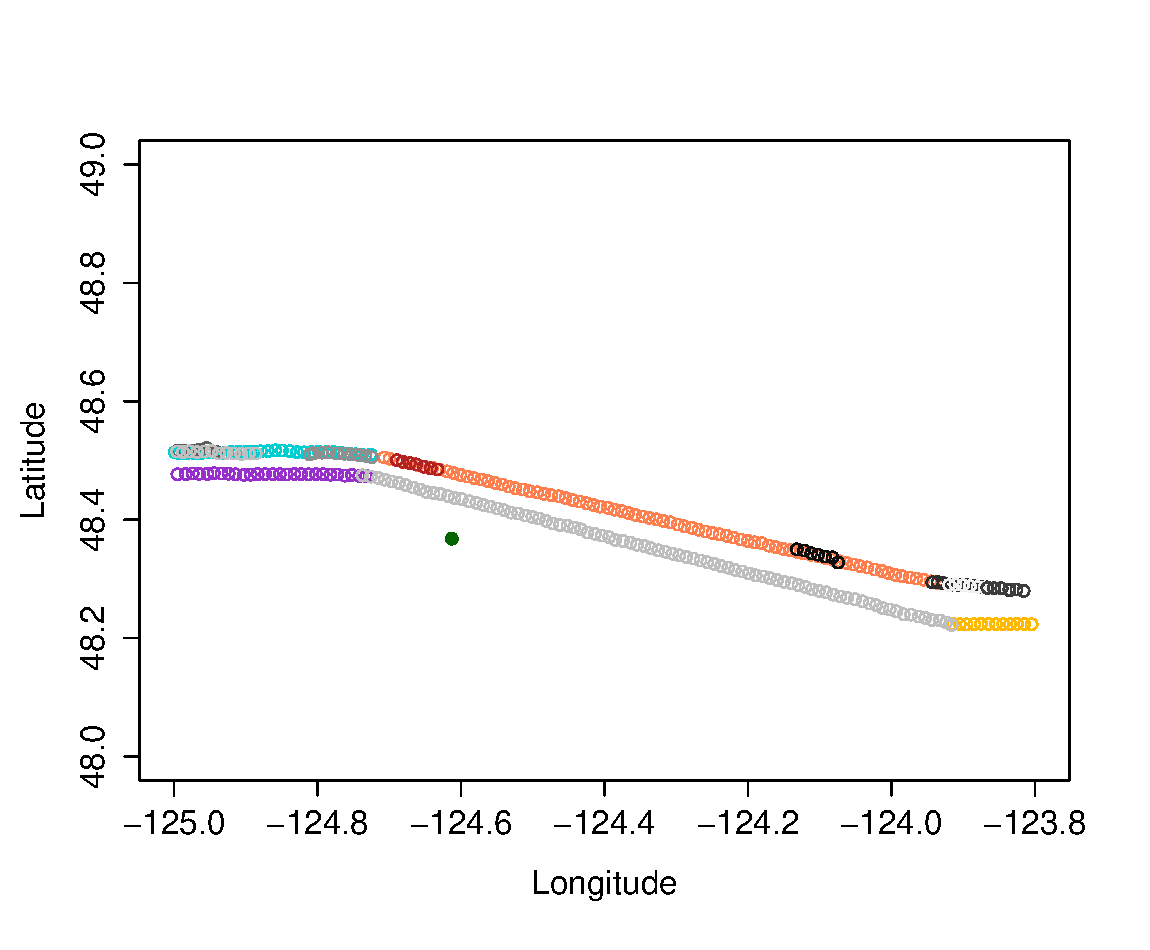
\includegraphics[width=8cm]{clusterGV.eps}
% \caption{The Gravity Vectors and Sampled Stopping Points extracted from the clusters in JUAN DE FUCA STRAIT area.}
% \label{fig:jdfk_gv}
% \end{figure}
\begin{figure}[!htb]
\centering
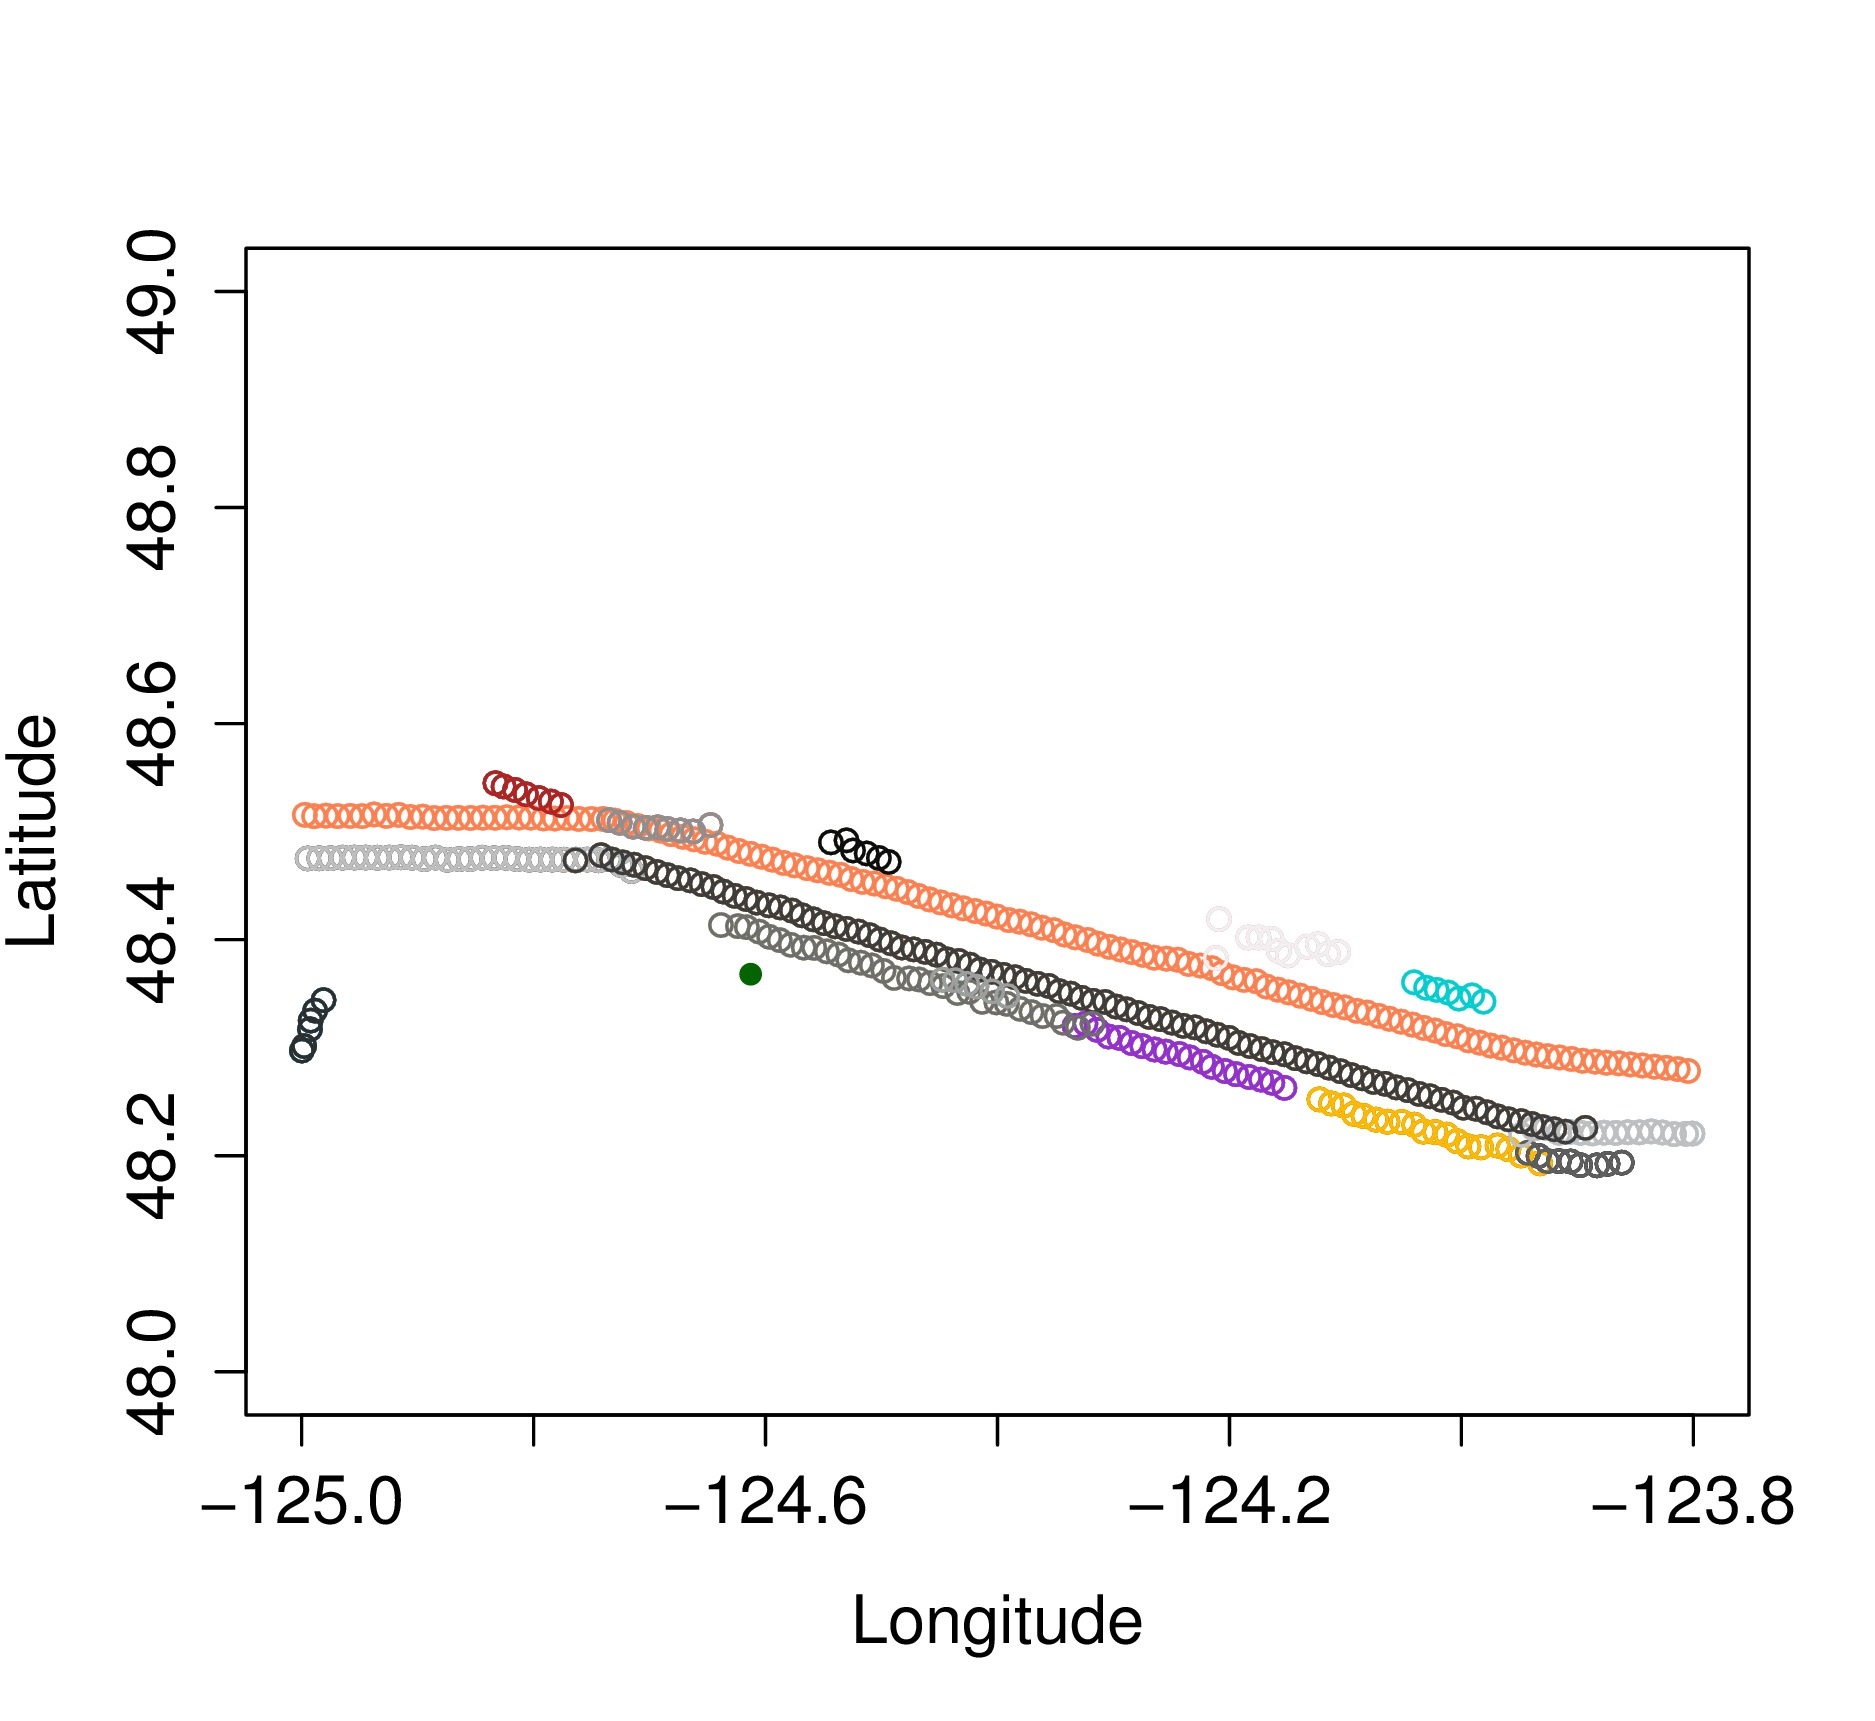
\includegraphics[width=5in,height=4.1in]{jdfk_clusters_new.jpg}
\caption{The Gravity Vectors (open circles) and Sampled Stopping Points (filled circles) extracted from the clusters in JUAN DE FUCA STRAIT area.}
\label{fig:jdfk_gv2}
\end{figure}

The next step before detecting anomalous trajectories is to estimate the three thresholds ($add\_threshold$, $rdd\_threshold$, $cdd\_threshold$) to be used in Algorithm \ref{algo3}. As stated before, the remaining 21,850 trajectory records  are chosen for this phase. There are 10,825 stopping points and 11,025 moving points in this subset.

The quartile values of ADD and RDD of the subset are shown in Table \ref{tb:tb1} (column 1 and column 2).
%%%add with Stan's suggestions
%Since this is an unsupervised work and we do not have labels for training the model, we have an assumption that $95\%$ of the data is normal in relation to distance and among these $95\%$ is normal in relation to speed and direction. The percentage of $95\%$ is decided by multiple tests and we finally employ $95\%$ in this work because it can detect a small number of anomalous trajectory points which can be analyzed by experts. The percentage can be varied according to different geo-spatial environments, in this case, the percentage of $95\%$ is rather high because the region is a strait and not many vessels are expected to navigate unconventionally. But if it comes to a more complicated open area, the percentage may be reduced theoretically.  %Based on the observation of the figures,
The authors tested different thresholds to be used as the anomaly detector. After various tests, for the area of Strait of Juan de Fuca the best threshold value was to consider $95\%$ of the data as normal in relation to distance, and from this sub-set another $95\%$ of the data to be considered normal in relation to speed and direction. The main objective is to reduce the number of false alarms (vessels considered abnormal, while they are normal), and this filtered data will later be evaluated by a human expert that will give the final decision. The model is flexible to allow changing this threshold value depending on the geographical area under evaluation.

 So we choose the sample quantiles of 0.95 for both ADD and RDD. The corresponding thresholds in this case, $add\_threshold$ and $rdd\_threshold$ in Algorithm \ref{algo3}, are 97.290 and 5.938. After calculating the RDD threshold, the statistic for CDD is obtained (shown in the 3rd column in Table \ref{tb:tb1}). Then we select 0.05 as the possibility to decide the third threshold (0.485) which can be employed as our CDD threshold ($cdd\_threshold$ in Algorithm \ref{algo3}). 

% \makeatletter
% \def\hlinew#1{%
%   \noalign{\ifnum0=`}\fi\hrule \@height #1 \futurelet
%   \reserved@a\@xhline}
% \makeatother
% \begin{table}
% \centering
%     \caption {Quartile statistics of the 3 division distances}
%     \begin{tabular}{lllr}
%     \hlinew{1pt}
%     Statistic    & ADD       & RDD       & CDD       \\
%     \hline
%     Min          & 0.00      & 0.02077   & -0.8792   \\
%     1st Quantile & 2.78      & 0.68119   & 0.7806    \\
%     Median       & 4.35      & 1.07272   & 0.8976    \\
%     Mean         & 36.71     & 3.09427   & 0.8568    \\
%     3rd Quantile & 62.00     & 2.11302   & 0.9671    \\
%     Max          & 40911.42  & 56.78009  & 1.0000    \\
%     \hlinew{1pt}
%     \label{tb:tb1}
%     \end{tabular}
% \end{table}
\makeatletter
\def\hlinew#1{%
  \noalign{\ifnum0=`}\fi\hrule \@height #1 \futurelet
   \reserved@a\@xhline}
\makeatother
\begin{table}
\centering
    \caption {Quartile statistics of the three division distances}
    \begin{tabular}{lllr}
    \hlinew{1pt}
    Statistic    & ADD       & RDD       & CDD       \\
    \hline
    Min          & 0.13      & 0.00537   & -0.9937   \\
    1st Quartile & 3.00      & 0.70300   & 0.7642    \\
    Median       & 4.46      & 1.04000   & 0.8876    \\
    Mean         & 36.97     & 1.81500   & 0.8104    \\
    3rd Quartile & 6.89     & 1.58400   & 0.9612    \\
    Max          & 44250.00  & 52.86000  & 0.9999    \\
    \hlinew{1pt}
    \label{tb:tb1}
    \end{tabular}
\end{table}

With the extracted normal patterns and the thresholds estimated, we start to evaluate the capacity for detecting abnormal trajectories. 


% \begin{figure}[!htb]
% \centering
% \includegraphics[width=8cm]{anomalyDetection.eps}
% \caption{The anomaly labeling results of the trajectory data points in JUAN DE FUCA STRAIT area.}
% \label{fig:anomalydetection_points}
% \end{figure}

\begin{figure}[!htb]
\centering
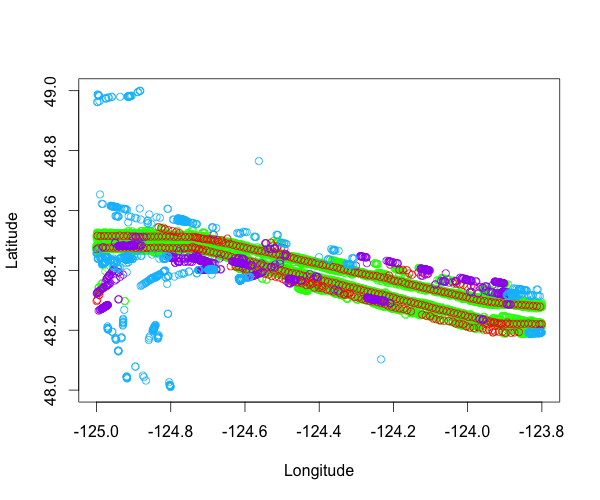
\includegraphics[width=5in]{labelJDFK.png}
\caption{The anomaly labeling results of the trajectory data points in JUAN DE FUCA STRAIT area. GVs and SSPs are in red and the normal points are in green. The two types of abnormal points are in blue (abnormal in relation to ADD or RDD) and purple (abnormal in relation to CDD).}
\label{fig:anomalydetection_points}
\end{figure}

In this step, we first apply our model to the trajectory data points; the labeling results of the data points are shown in Figure \ref{fig:anomalydetection_points}. The red points stand for the GVs and the SSP in this area. The green points are normal, while the blue and purple ones are abnormal. More specifically, a blue point means it is too far away from the corresponding GV or SSP, while a purple point represents that its speed or direction is aberrant in the specific location.  In this case, 1,534 points (872 in blue and 662 in purple) of the 17,431 points are finally considered as abnormal. 

After finishing the labeling process, we calculate the abnormality ratio of each trajectory. We use a threshold of 0.5 as the minimum confidence rate to extract the abnormal trajectories. Noteworthy, the number 0.5 is adjustable and was chosen based only on the experiments to reduce the presence of false alarms (normal trajectories considered abnormal by our model). The result is that 22 trajectories are labeled abnormal among the total 284 trajectories. In other words, the abnormality rates of these 22 trajectories are over 0.5. From Figures \ref{fig:anomalydetection_tra1} to \ref{fig:anomalydetection_tra6}, six examples of abnormal cases are illustrated. As can be seen in the figures, both purple points and blue points contribute to the final abnormality of one trajectory.



% \begin{figure}[!hp]
% \centering
% %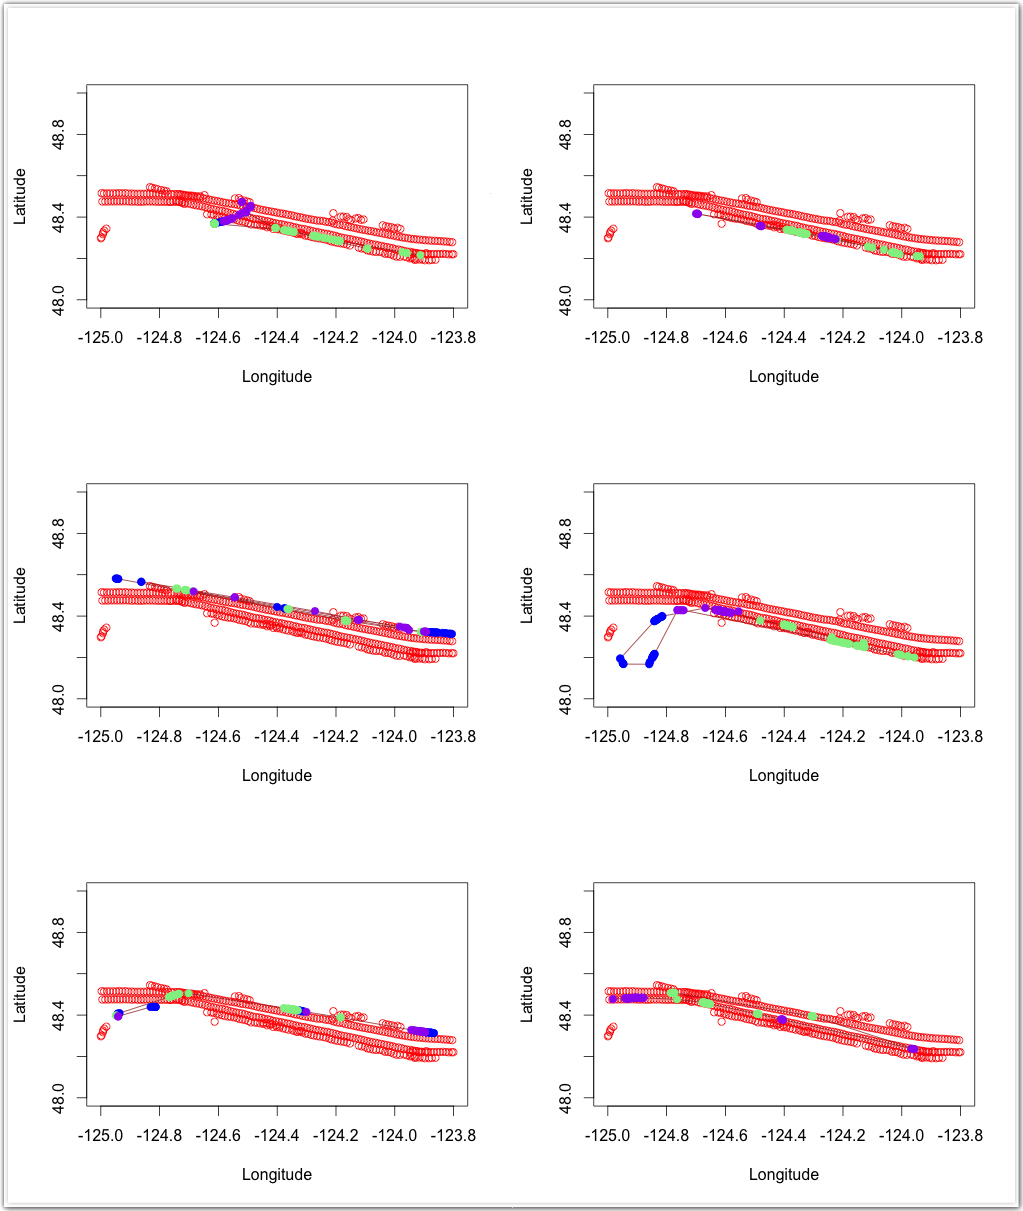
\includegraphics[height=12cm]{anomalyExamples.jpg}
% 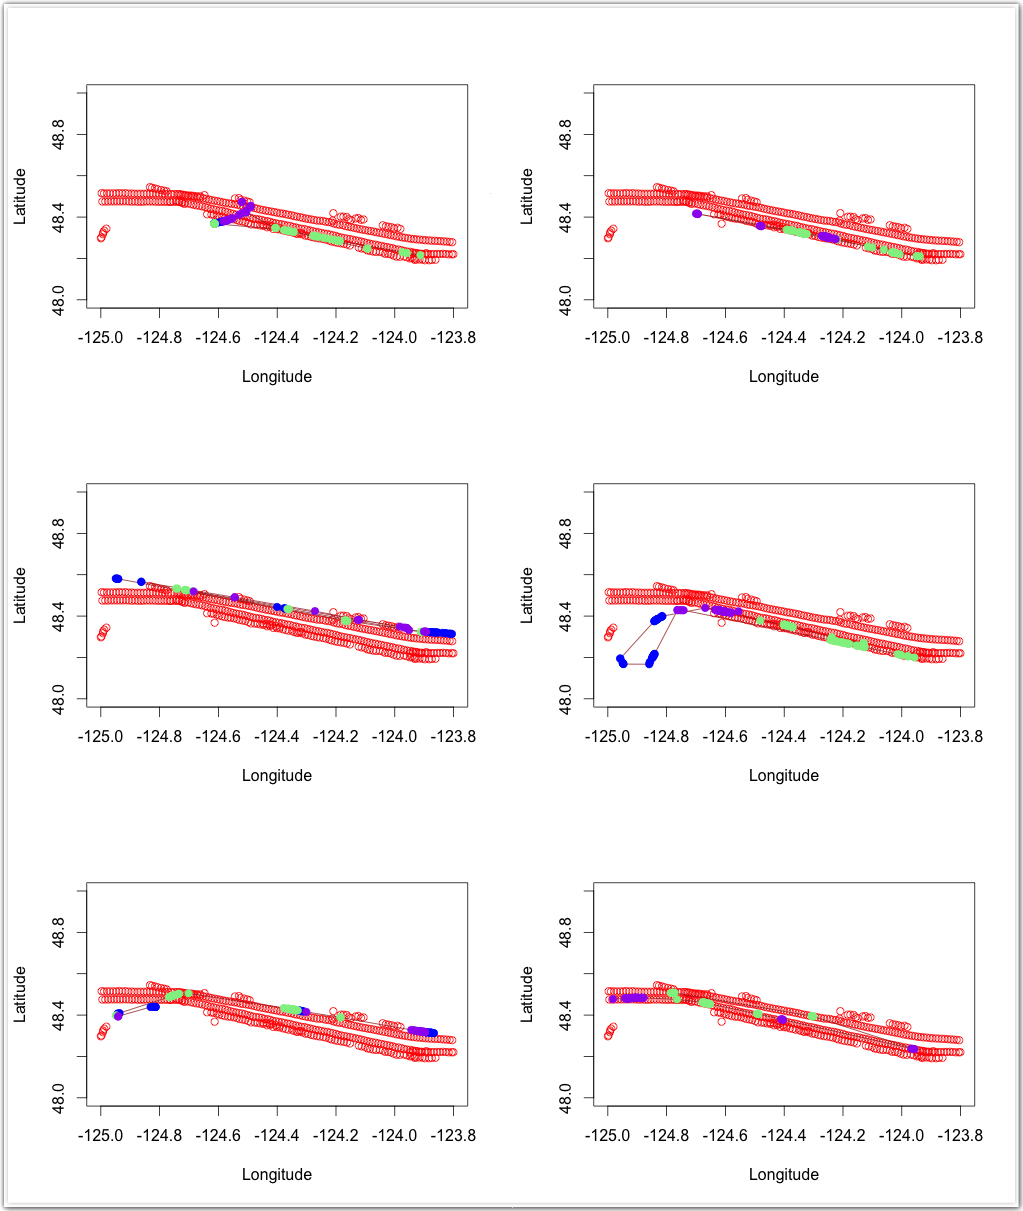
\includegraphics[width=5.8in,height=7.8in]{anomalyExamples.jpg}
% \caption{Six Examples of the abnormal trajectories detected by our framework in JUAN DE FUCA STRAIT area.}
% \label{fig:anomalydetection_tra}
% \end{figure}

\begin{figure}[!hp]
\centering
%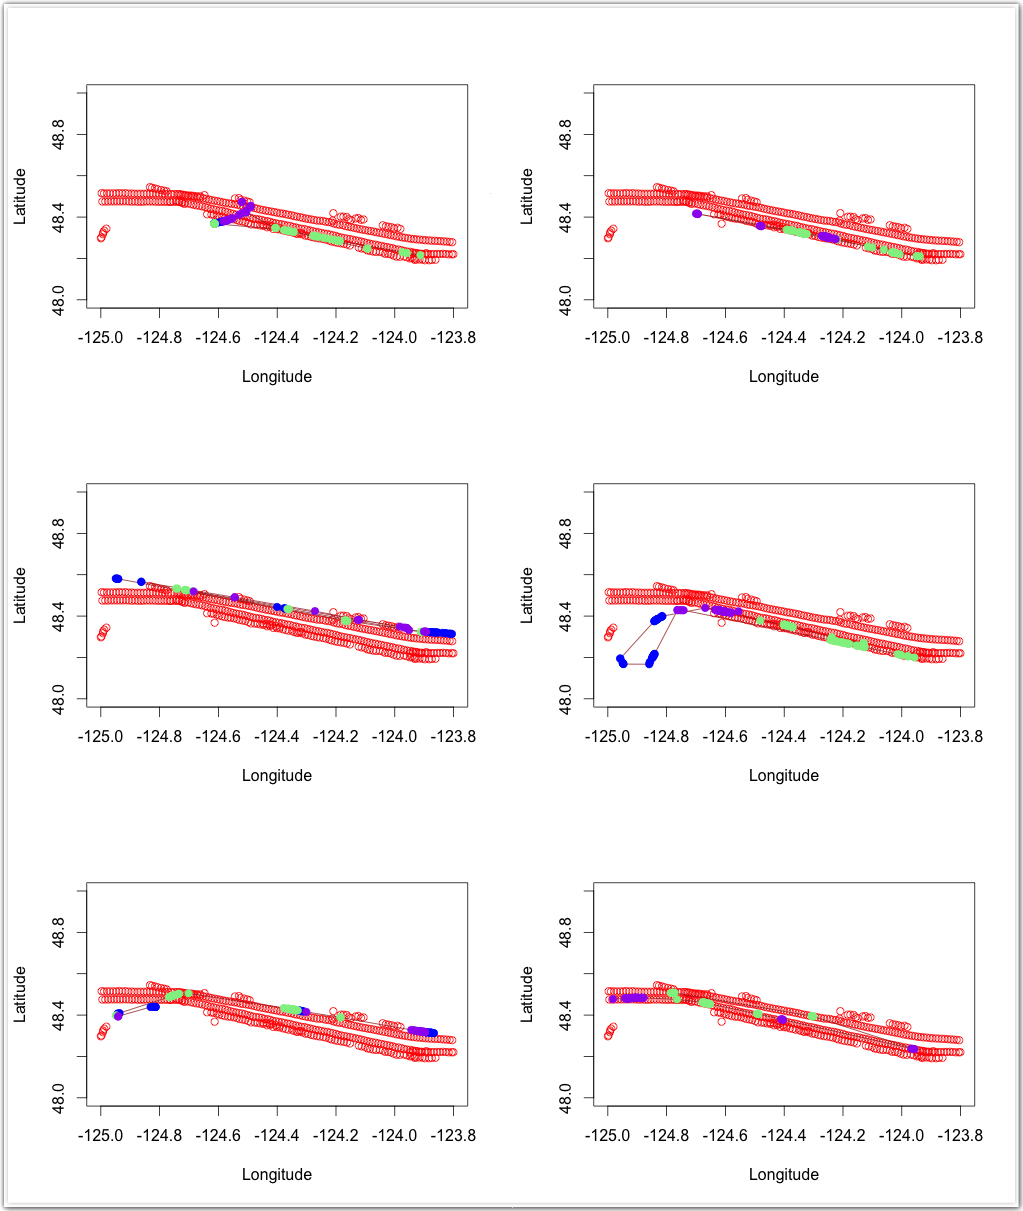
\includegraphics[height=12cm]{anomalyExamples.jpg}
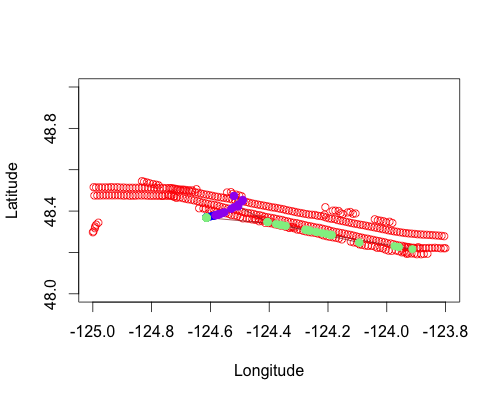
\includegraphics[width=4.1in, height=3.3in]{p1.png}
\caption{First example of the abnormal trajectories detected by our framework. GVs and SSPs are in red and the normal points are in green. The two types of abnormal points are in blue (abnormal in relation to ADD or RDD) and purple (abnormal in relation to CDD).}
\label{fig:anomalydetection_tra1}
\end{figure}

\begin{figure}[!hp]
\centering
%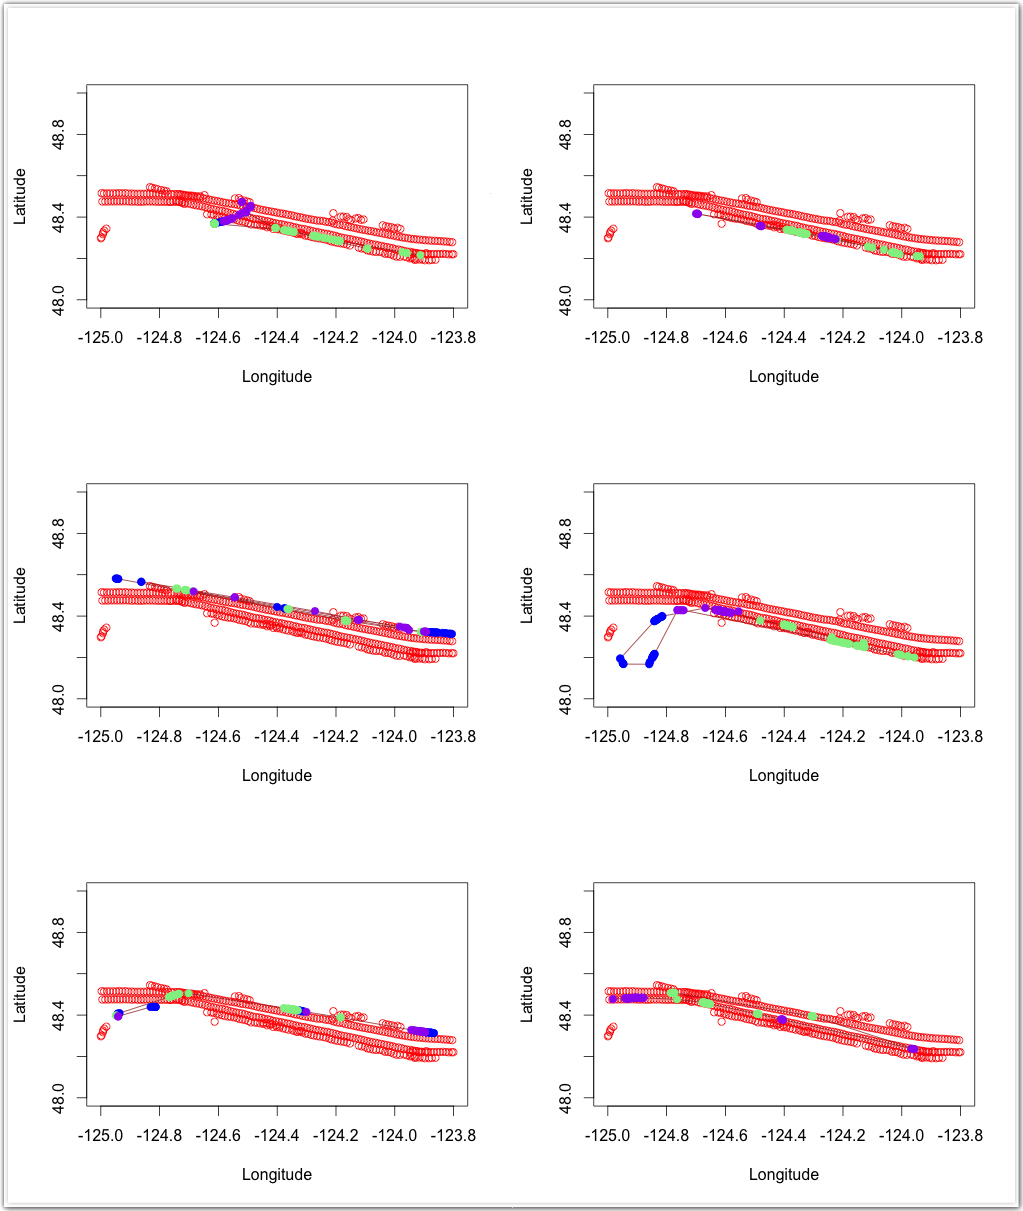
\includegraphics[height=12cm]{anomalyExamples.jpg}
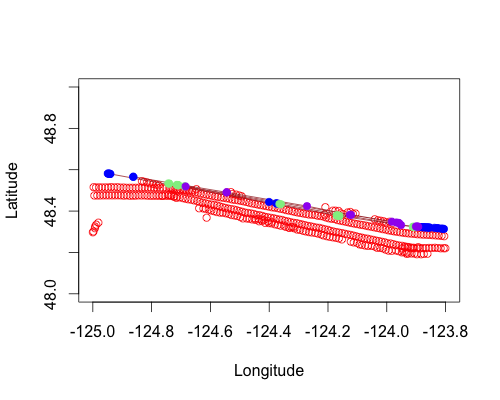
\includegraphics[width=4.1in, height=3.3in]{p2.png}
\caption{Second example of the abnormal trajectories detected by our framework. GVs and SSPs are in red and the normal points are in green. The two types of abnormal points are in blue (abnormal in relation to ADD or RDD) and purple (abnormal in relation to CDD).}
\label{fig:anomalydetection_tra2}
\end{figure}

\begin{figure}[!hp]
\centering
%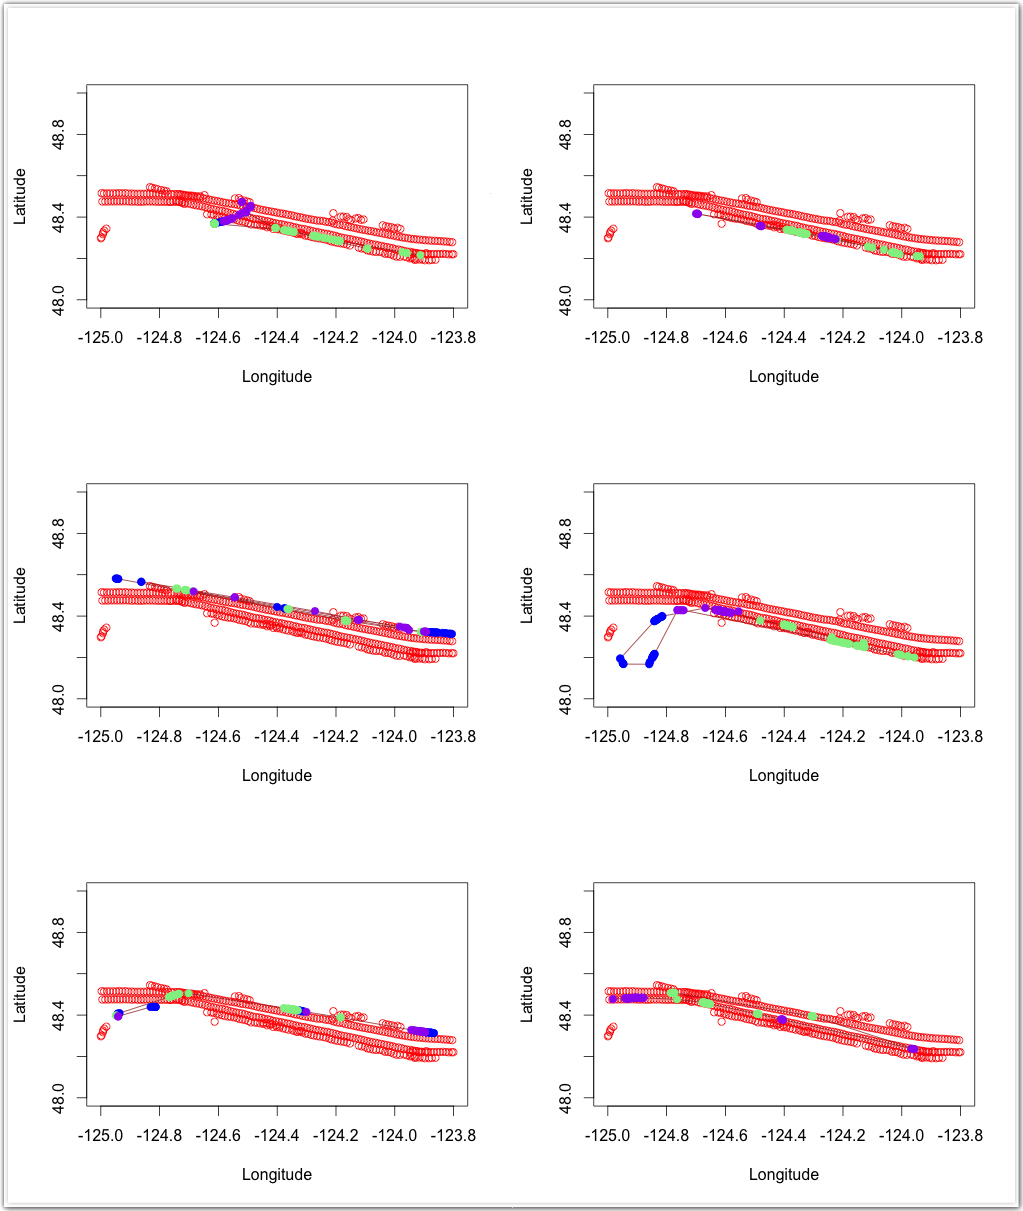
\includegraphics[height=12cm]{anomalyExamples.jpg}
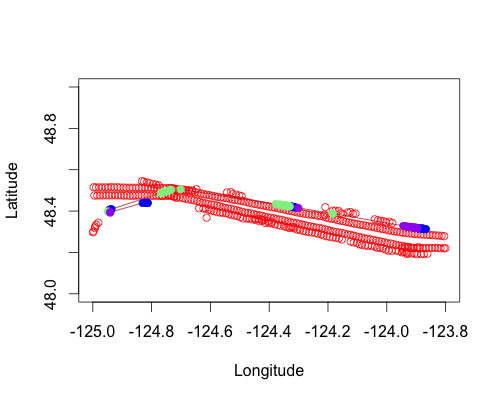
\includegraphics[width=4.1in, height=3.3in]{p3.png}
\caption{Third example of the abnormal trajectories detected by our framework. GVs and SSPs are in red and the normal points are in green. The two types of abnormal points are in blue (abnormal in relation to ADD or RDD) and purple (abnormal in relation to CDD).}
\label{fig:anomalydetection_tra3}
\end{figure}

\begin{figure}[!hp]
\centering
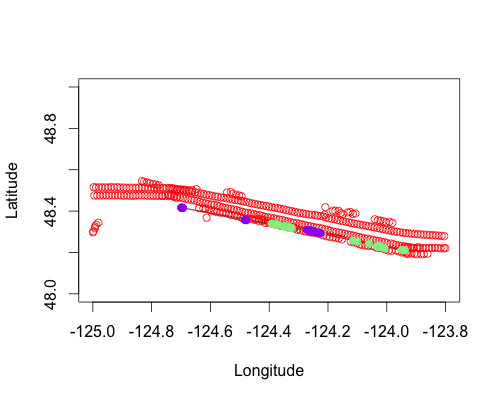
\includegraphics[width=4.1in, height=3.3in]{p4.png}
\caption{Fourth example of the abnormal trajectories detected by our framework. GVs and SSPs are in red and the normal points are in green. The two types of abnormal points are in blue (abnormal in relation to ADD or RDD) and purple (abnormal in relation to CDD).}
\label{fig:anomalydetection_tra4}
\end{figure}

\begin{figure}[!hp]
\centering
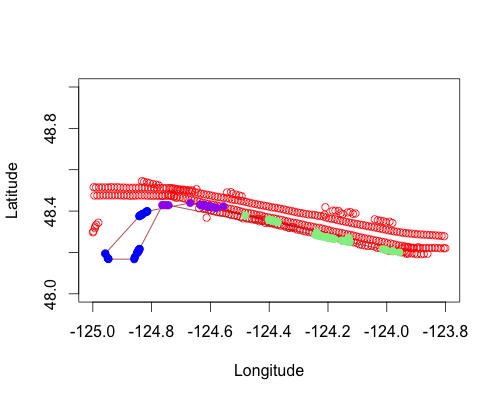
\includegraphics[width=4.1in, height=3.3in]{p5.png}
\caption{Fifth example of the abnormal trajectories detected by our framework. GVs and SSPs are in red and the normal points are in green. The two types of abnormal points are in blue (abnormal in relation to ADD or RDD) and purple (abnormal in relation to CDD).}
\label{fig:anomalydetection_tra5}
\end{figure}

\begin{figure}[!hp]
\centering
%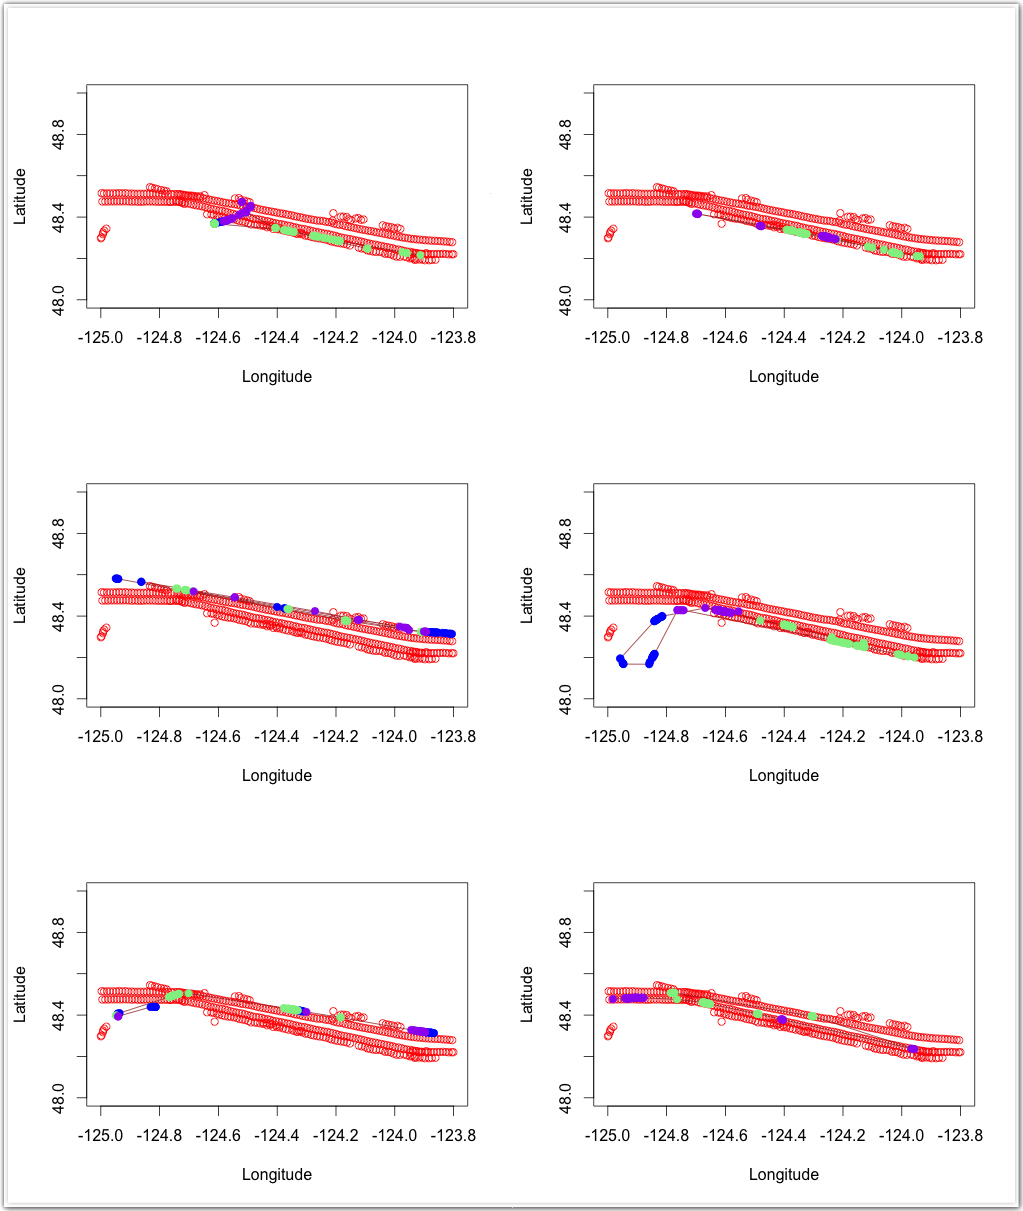
\includegraphics[height=12cm]{anomalyExamples.jpg}
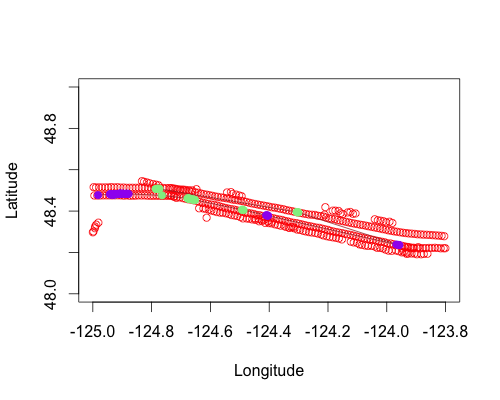
\includegraphics[width=4.1in, height=3.3in]{p6.png}
\caption{Sixth example of the abnormal trajectories detected by our framework. GVs and SSPs are in red and the normal points are in green. The two types of abnormal points are in blue (abnormal in relation to ADD or RDD) and purple (abnormal in relation to CDD).}
\label{fig:anomalydetection_tra6}
\end{figure}



\subsection{Experiment On Labeled Data Set}
\label{sec:exp_2.2}
In this experiment, the same data set is labeled by an expert who has multiple years of experience in maritime data analysis. The labelling process is not biased by our model's results since only the raw AIS data has been provided to the expert. 


\begin{table}[!htb]
\centering
    \caption {Labels and descriptions by the expert}
    \begin{tabular}{cl}
    \hlinew{1pt}
    Label    & Description\\
    \hline
    
    $Bad\_Pos$      &Track contains questionable point, far outside \\&track, looks like bad GPS return\\
    $In\_Excl\_Zn$ & Track has significant portion within the exclu-\\& sionary zone between traffic lanes \\
    $XING\_TSS$  & Track appears to be crossing lanes of TSS \cite{tss}    \\
    $XING\_NShor$   & Track appears to be crossing lanes of near sh- \\& ore two way traffic area    \\
    $Odd\_Mvmt$ & Track shows unusual movement without other\\& explanation\\
    $Leave\_Lane$   & Vessel was in traffic lane, then veered outside    \\
    $Harbour$      & Track seems to describe in-harbour navigation\\& or moored vessel    \\
    $Normal$      & Normal Movement   \\
    \hlinew{1pt}
    \label{tb:tb2}
    \end{tabular}
\end{table}

A track division method is employed by the expert before labelling. More specifically, the AIS data points are divided into distinct tracks on the basis of vessel ID (MMSI), and where temporally sequential points are separated by no more than 4.5 minutes of time.
%tracks are divided based on an equal time interval, which is assumed 4.5 minutes. 
Thus one track, as defined above, may be divided into multiple-sub tracks on the basis of time. Additionally, this process can result in tracks comprised of single points.
%Thus one track can be divided into multiple sub-tracks and there can also be one track composed by merely one point. 
For the one-point track case, the length of the track is 0 nautical mile and the track is not assigned with any labels. The final labels and their descriptions provided by the expert are shown in Table \ref{tb:tb2}. 


The labels assigned by the expert are not based on the points; instead, they are based on the whole sub-tracks. In other words, as long as one sub-track shows an anomalous pattern, the whole set of points inside the sub-track will be assigned as one kind of abnormal label. Another noteworthy point is that the expert has not taken SOG (speed) into account except for Harbour behavior during his labeling process. That is, whether the speed of the vessel is too fast or too slow near the lane is not considered, but our algorithm can take this into account.

From Table \ref{tb:tb2}, we can firstly assume the label of $Normal$ as normal patterns based on the description. Then the label $Harbour$ can also be considered as a normal case because it is reasonable for a vessel to moor in harbour. Lastly, we observe that all the sub-tracks with the label of $Leave\_Lane$ only have tiny changes from their route and they still navigate strictly within the normal lanes. So we also classify the label of  $Leave\_Lane$ as normal.

After dividing the 284 tracks (284 different MMSIs), 2,122 sub-tracks are generated. Among them, 680 sub-tracks contain only one point (Length=0 nautical mile). Then 14 sub-tracks are classified as abnormal labels (other than $Leave\_Lane$, see Table \ref{tb:tb2}) by the expert and the remaining 1,428 tracks are all normal patterns. Thus we can see that the data set is a highly imbalanced data set which can make our work extremely challenging. 

%According to the expert, a new version of IMO rules is used for labeling the data. The new version involves another two-way route which is located South of the original main route. Thus we first adjusted the parameters used in our normal traffic lanes extraction model to update the clusters and Figure \ref{fig:jdfk_clusters_new} shows the new clustering result.


% \begin{figure}[!htb]
% \centering
% 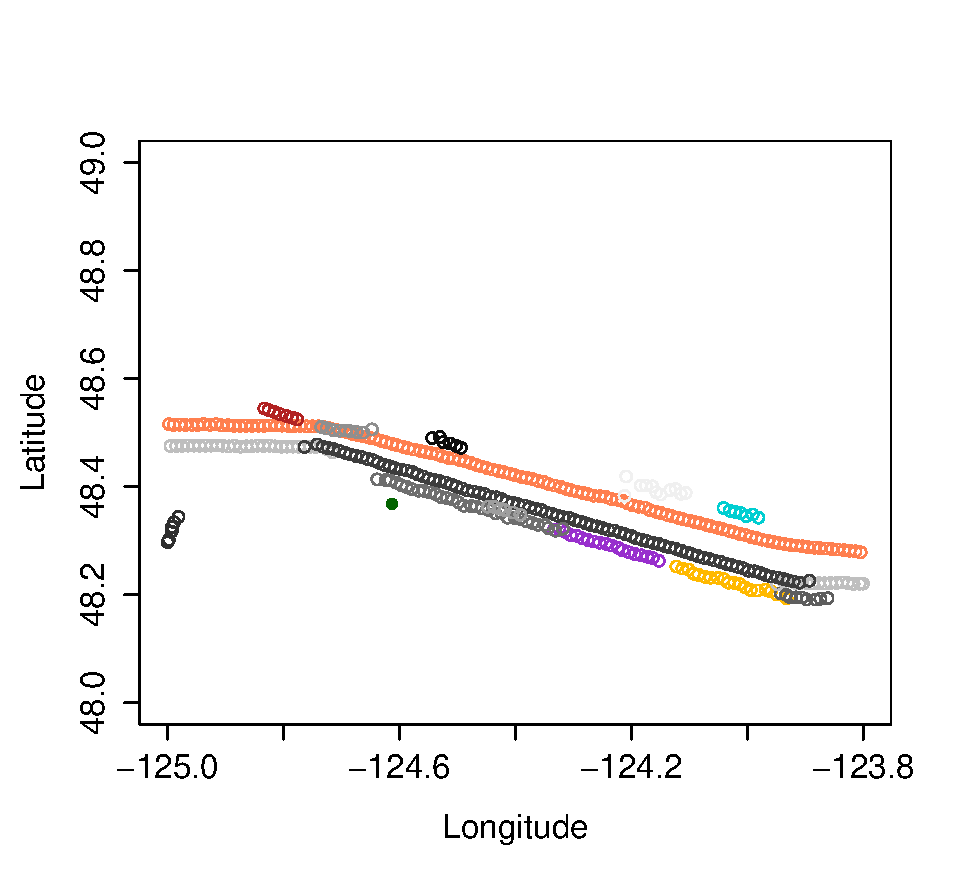
\includegraphics[width=8.5cm, height=7cm]{jdfk_clusters_new.eps}
% \caption{The new clustering result of the trajectory data points in JUAN DE FUCA STRAIT area.}
% \label{fig:jdfk_clusters_new}
% \end{figure}


At this point we can use our algorithm to label the data set and compare the results with the expert's labels. To compare the results, we first apply the same division method to separate the tracks. We can then use a threshold to decide the whole sub-track's label. In this experiment, we employ $60\%$ as the threshold value. That means that if the portion of abnormal points in one track is greater than $60\%$, we will label this whole track as abnormal. Using this approach, we find that 131 sub-tracks are classified as abnormal and the remaining 1,311 sub-tracks are normal. Table \ref{tb:tb3} is the confusion matrix for the experiment.

\begin{table}
\centering
    \caption {Confusion Matrix I}
    \begin{tabular}{ccc}
    \hlinew{1pt}
        & Abnormal  & Normal\\
        & (Our Model) &(Our Model)\\
    \hline
    Abnormal (Expert's Label) & 4      & 10\\
    Normal (Expert's Label) & 127      & 1301      \\
    \hlinew{1pt}
    \label{tb:tb3}
    \end{tabular}
\end{table}

From Table \ref{tb:tb3} we can see that 4 sub-tracks are classified as abnormal by both the expert and our model and 1301 sub-tracks are classified as normal by both too. On the other hand, another 10 sub-tracks are labeled as abnormal by the expert while normal by our model. The remaining 127 sub-tracks are classified as abnormal by our model while normal by the expert.  And the overall accuracy of this detection result is $90.49\%$.

\begin{table}
\centering
    \caption {Confusion Matrix II}
    \begin{tabular}{ccc}
    \hlinew{1pt}
        & Abnormal  & Normal\\
        & (Our Model) &(Our Model)\\
    \hline
    Abnormal (Expert's Label) & 4      & 10\\
    Normal (Expert's Label) & 52      & 1376      \\
    \hlinew{1pt}
    \label{tb:tb4}
    \end{tabular}
\end{table}

%To improve the result, we investigate the 14 sub-tracks designated as abnormal by the expert. The algorithm detect only 4 of these tracks as abnormal, only because of their direction.

To improve the result, we investigate the 14 sub-tracks designated as abnormal by the expert. Among these, we find that the 4 which are further designated as abnormal by the algorithm are so labeled solely because of their direction. After investigating other tracks, we find that
even if the ships deviate far from the lane the expert may still label them as normal. The intuition behind this is straight-forward, as the labelling process is based on Traffic Separation Scheme (TSS) \cite{tss} boundaries and the expert cannot affirm that a trajectory point far from the TSS Boundaries is abnormal. %Instead, the factor of direction plays a more significant role and ships should navigate in the right direction while they are inside the lanes to avoid collision.
Considering this fact, in the following experiment, we ignore the abnormal labels caused by RDD or ADD during the evaluation and we choose a lower threshold for deciding  whole sub-tracks' labels. In the previous experiment we use $60\%$ while we choose $10\%$ here. It should be noted that the threshold can be adjusted based on the input from domain experts. In real-time application, it is not necessary to have the threshold while labelling the new incoming points instead of tracks.

Table \ref{tb:tb4} presents the improved results and we can see that the overall accuracy has been increased from $90.49\%$ to $95.70\%$ while keeping the same recall for abnormal cases.




\chapter{Conclusion}
\label{ch:conclusion}


In this thesis, a maritime traffic pattern extraction model has been first proposed. The approach first separates the trajectory data set into moving and stopping subsets, and then employ different strategies in corresponding subsets. The main advantage of this work is that two attributes, speed and direction, are taken into account during the clustering phase. In this way, geographically close trajectory points with similar direction and speed can be grouped together to form a cluster. We also present two methods to represent the results of clustering; that is, Gravity Vector for moving clusters and Sampled Stopping Point for stopping clusters.  %Another contribution of this work is that it can map the clustering results to the rules defined by the IMO publications.

Another contribution of the proposed normal traffic extraction model is that it can be easily extended for other scenarios. Besides the maritime anomaly detection task addressed in this thesis, the moving trajectories clustering algorithm (DBSCANSD) and Gravity Vectors are also applicable for other trajectory clustering tasks (e.g. vehicle position data, animal movement data, hurricane monitoring data). Thus, more experiments can be done with other domains' data sets to verify our method's applicability in the future study.

To show the effectiveness of our approach, two real data sets from different regions (Juan de Fuca Strait area and Los Angeles Long Beach area) are used. We have compared the generated results with the rules defined by IMO and it shows that the results can be successfully mapped to the rules. This demonstrates that our model can effectively mine normal patterns in the two areas, which is another contribution of this work.

One limitation of the normal traffic extraction model is that it is sensitive to parameters. The model requires four parameters ($eps$, $MinPts$, $MaxDir$, $MaxSpd$) during the moving traffic patterns extraction phase and two parameters ($eps$ and $MinPts$) for stopping area generation. So, if the model is applied in another area, a new set of parameters needs to be given to achieve a good clustering result. Thus, to achieve satisfactory clustering results, it is necessary to possess a good maritime background. Specifically, when we distinguish moving points from stopping points in the first step, a reasonable SOG threshold is required. Here in this thesis, we adopt 0.5 knots as the threshold for distinguishing stopping and moving. Besides, before applying DBSCANSD to moving trajectory points, we cannot simply assume the tolerated angle ($MaxDir$) between two close points' directions and the tolerated difference ($MaxSpd$) between two close points' speeds.

%a vessel's direction and the normal direction. 

%the framework  relies on the users' domain knowledge.  Beyond the definition of the 4 parameters for the clustering algorithms, , as well. For example, 





The Gravity Vectors and Sampled Stopping Points detected by the proposed approach can help authorities update their rules (e.g. re-position the buoy markers).  Some other research studies like route planning and vessel position prediction can also be conducted based on our model's results. 


Based on the Gravity Vectors and Sampled Stopping Points extracted from the clustering phase, we then propose the anomaly detection model for maritime traffic data. An abnormality detection algorithm is presented based on three division distances (Absolute Division Distance, Relative Division Distance and Cosine Division Distance). This model is a fairly straightforward point-based approach, and is capable of handling complicated maritime traffic situations. One advantage is that the clustering process is associated with TSS Boundaries \cite{tss}, which can assure a reliable clustering result for the following anomaly detection work. Another critical advantage is that besides position information (Longitude and Latitude), the model can also take speed and direction into account while deciding the abnormality of a single trajectory point. The model is also flexible enough for analysts to set their own thresholds to label whole trajectories. 

In order to evaluate the effectiveness of the anomaly model, a highly imbalanced data set from Juan de Fuca Strait area is used. There are 2,122 trajectories while only 14 of them are abnormal (imbalance rate $\approx$ 0.66$\%$). Fortunately, as shown in Table \ref{tb:tb4}, our model can detect 28.57$\%$ of the abnormal tracks while maintaining a relatively high overall accuracy (95.70$\%$).



%The first reason is that there is not enough labeled data. As mentioned in Section IV, the data is highly-imbalanced and there are merely 14 anomalous tracks, which is infeasible to train an effective model for anomaly detection. %Secondly, from the experiment section we can see our unsupervised framework achieves a satisfactory result

%One limitation of the  anomaly detection evaluation model is that the labelling process applied by the expert does not consider speed while our work takes this into account. This leads to another possible future direction, that is, more work should be done by the experts while labelling the data set to consider speed. And in this way, the false alert rate can also be reduced while the recall of the anomaly trajectories is improved. Another limitation is that the experiments are only conducted with data from Juan de Fuca Strait area and as a result, more experiments in other regions should be done to better illustrate the effectiveness of our approach.

%Secondly, the labelling process applied by the expert does not consider speed while our work takes this into account. So if we train the model based on the labeled data, we cannot get a model to detect anomalous behaviours in relation to speed. However, this also leads to a possible future direction, that is, more work should be done while labelling the data set to consider speed. 








%Routes prediction:




\section{Future Work}

%% MSYD
One of the possible directions of future work is to improve the efficiency of the presented algorithms by applying more sophisticated data structures (like spatial indexes, for example). This issue is important in the context of big sizes of the processed data. In this thesis the focus was not on optimising the efficiency of the algorithms but to present the ideas. We envisage algorithm optimisation in the future work.
%%

One may argue about the use of an unsupervised learning approach instead of supervised learning methods. The reason for this is that there is  insufficient labeled data to train an effective model. Once we get enough labeled data we will explore other supervised learning techniques for this anomaly detection task. For example, we can try some classification algorithms designed for handling imbalanced data sets and the proposed specialized division distances can be used as the features of the classification models.  Then comparisons between those results and our model's outcomes could be done to illustrate the effectiveness of the proposed division distances.

One limitation of the  anomaly detection evaluation model is that the labelling process applied by the expert does not consider speed while our work takes this into account. This leads to another possible future direction, that is, more work should be done by the experts while labelling the data set to consider speed. In this way, the false alert rate can also be reduced while the identification of the anomaly trajectories is improved. Another limitation is that the experiments are only conducted with data from Juan de Fuca Strait area and as a result, more experiments in other regions should be done to better illustrate the effectiveness of our approach.




\begin{figure}[!htb]
\centering
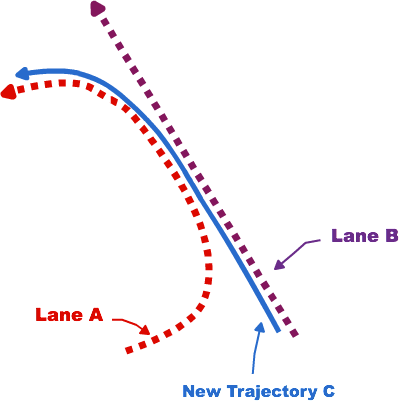
\includegraphics[width=4in,height=3.5in]{limitation3.png}
\caption{One situation that our algorithm cannot detect the anomalies. Two normal lanes (Lane $A$ and Lane $B$) detected by DBSCANSD are in red and purple. A new anomaly trajectory $C$ is in blue.}
\label{fig:limitation3}
\end{figure}


As discussed before, this is a point-based method and the output is two sets of representative vectors (Gravity Vectors and Sampled Stopping Points). As a consequence, one limitation of our clustering algorithm, compared to trajectory-based ones, is that ours cannot take into account the behavior over time.  One example of this limitation is illustrated in Figure \ref{fig:limitation3}. Assume there are two main lanes in the region and they are Lane $A$ and Lane $B$ (shown in red color and purple color separately). Then a vessel enters the region and follows a path such as Trajectory $C$. Since our framework treats the trajectories as sequences of data points, the trajectory will be divided into two sub-sequences and during anomaly detection phase, the first part will be associated with Lane $B$ while the second part will be associated with Lane $A$. In this sense, the new trajectory will be assigned as normal. However, the vessel is not supposed to change its navigational lane once it starts its trip on Lane $B$ because there are only two shipping routes pre-defined in this region. So in this situation, our model fails to detect the new anomaly trajectory $C$, and this can be improved after considering time, which is one aim of our future work.


The clustering results of the first phase can be used for predicting vessels' routes. Since the GVs extracted carry not only the position information (Longitude and Latitude) but also the kinematic characteristics (course and average speed), it is feasible for researchers to obtain the corresponding expected speed and heading for the specific predicted position. Two potential ways for handling this can be association rules mining techniques or Bayesian approaches. As stated in Chapter \ref{ch:background}, anomaly detection approaches based on predictive models usually predict future status information of a particular vessel and then compare the real data with the prediction to decide the abnormality. Thus, to improve the performance of the model, an ensemble model which incorporates the predictive model can be developed in the future. Specifically, once a trajectory point needs to be labeled, we can consider both its anomalous score (output of our proposed model) and its deviation from the predicted position to get a more confident result. 



% %%%abreviations

% SOG - Speed Over Ground
% COG - Course Over Ground
% GV - Gravity Vector
% SSP - Sampled Stopping Point
% AIS - Automaitc
% IMO-
% GPS
% DBSCAN
% ADD
% RDD
% CDD

% TSS Traffic Separation Scheme boundaries
% DTW
% PDF
% KDE
% GMM

\bibliographystyle{plain}
\bibliography{simple}



%\let\cleardoublepage\clearpage
%\cleardoublepage\makeatletter\@openrightfalse\makeatother

\appendix
%\let\cleardoublepage\clearpage

\chapter{Source Code of the Algorithms}
%\let\cleardoublepage\clearpage

In this appendix, some key source code implemented during the thesis is shown. The whole framework is divided into two parts: normal traffic patterns extraction model and anomaly detection model. The first part shown in \ref{code1} has been mostly implemented in Java with a small portion of R code. While the second part shown in \ref{code2} has been implemented totally in R. 

\section{Source Code of Normal Traffic Patterns Extraction Model}
\label{code1}

As discussed in Chapter \ref{ch:normal_traffic_extraction_model}, the normal traffic extraction model includes two different clustering components (DBSCANSD and DBSCAN) to handle moving trajectory points and stopping areas respectively. Before presenting the code for clustering, it is necessary to first define the classes of \textbf{Trajectory Point} and \textbf{Cluster}.

\lstinputlisting[language=Java, caption=Class of TrajecotryPoint,
    basicstyle=\footnotesize%\tiny, %or \small or \footnotesize etc.
]{./code/TrajectoryPoint.java}

The \textbf{cluster} defined in Definition \ref{def:cluster} is basically a set of trajectory points. So the Class of Cluster can be written as follows:

\lstinputlisting[language=Java, caption=Class of Cluster,
    basicstyle=\footnotesize%\tiny, %or \small or \footnotesize etc.
]{./code/Cluster.java}

\subsection{Code of Clustering Process}


The clustering process includes two steps which are DBSCANSD for moving points clustering and DBSCAN for stopping points clustering. The two steps have been implemented together in terms of the code's reusability (DBSCANSD can be regarded as an extension of DBSCAN). 

%set mathescape as true to make $--$ work as --, if we need that breqn package, we can keep this parameter here
\lstinputlisting[mathescape=true,language=Java, caption=The code of clustering process,
    basicstyle=\footnotesize%\tiny, %or \small or \footnotesize etc.
]{./code/DBScanSD.java}


\subsection{GVs Calculation}

In this section, the code of the algorithm to calculate a cluster's Gravity Vectors is given. First, as defined in Chapter \ref{ch:normal_traffic_extraction_model}, a Gravity Vector is a vector formed by 5 features: average COG, average SOG, average Latitude, average Longitude and Median Distance, the class of the \textbf{Gravity Vector} needs to be first presented. Here the GV is inherited from the Class of Trajectory Point  (Listing A.1). 

\lstinputlisting[language=Java, caption=Class of Gravity Vector,
    basicstyle=\footnotesize%\tiny, %or \small or \footnotesize etc.
]{./code/GravityVector.java}

As demonstrated in Chapter \ref{ch:normal_traffic_extraction_model}, the process of calculating GVs of a cluster needs to map the trajectory points to an axis of the average direction. So here a Class called Mapping Point is also given and it also inherits from the Class of Trajectory Point:

\lstinputlisting[language=Java, caption=Class of Mapping Point, basicstyle=\footnotesize]{./code/MappingPoint.java}

After having the Gravity Vector and Mapping Point classes, we can start to write the code for extracting the GVs from a given cluster. 

\lstinputlisting[language=Java, caption=Extract GVs from a cluster,basicstyle=\footnotesize%\tiny, %or \small or \footnotesize etc.
]{./code/GravityVectorExtraction.java}

\subsection{SSPs Calculation}

SSP (Sampled Stopping Point) is a type of points to represent the geo-spatial shape of a cluster and it does not need to consider the factors of speed or direction (See Section \ref{sec:normal_stopping_model}). Here the algorithm of extracting SSPs from stopping clusters (Algorithm \ref{algo2}) has been implemented in R.


\lstinputlisting[language=R, caption=Extract SSPs from stopping clusters, basicstyle=\footnotesize%\tiny, %or \small or \footnotesize etc.
]{./code/SSPExtraction.R}

\section{Source Code of Anomaly Detection Model}
\label{code2}

This section is focused on the anomaly detection labeling process. The algorithm uses as input the clusters described in previous sections, and uses them to generate a label that informs what type of anomaly was found. The algorithm associates labels to each AIS data point according to the following:

$\bullet$ \textbf{0} stands for distance abnormal

$\bullet$ \textbf{1} is normal

$\bullet$ \textbf{-1} is direction or speed abnormal

$\bullet$ \textbf{9} is data incomplete

The R function code, called labelAnomalyPointsWithStopMoveclusters, contains the function that is responsible for the labeling detection. Observe that this function uses other helper functions that are later described. The function inputs are the following:

$\bullet$ The inputData parameter is a data frame of the following format: (``MMSI'', ``SOG'', ``Longitude'', ``Latitude'', ``COG'');

$\bullet$ The normalPointsMove parameter is a data frame of the following format: (``clusterindex'', ``Longitude'', ``Latitude'', ``SOG'', ``COG'', ``QuartileDistance'')

$\bullet$ The normalPointsStop is a data frame with the following format: (``Longitude'',``Latitude'')

The algorithm first executes a check to guarantee that data is in correct format, by verifying if all required fields in inputData are complete. If they are not, the algorithm adds a label “9”, indicating that data is incomplete. This step guarantees that all AIS coordinates that have missing values are going to be labeled as incomplete. 

Next, the algorithm executes a function called generatefeaturesRelativeDistance, which generates a set of extra distance descriptors for the inputData parameter. This function is presented in next section. These distances will be used to rank which AIS points are more abnormal than others.  The function getIndexOfFarPointsRELATIVE calculates which points are abnormal in relation to distance from the clusters.  This function uses two extra parameters as threshold to indicate the anomaly. These values were empirically found during clustering steps.

If the points are still normal in relation to distance from the clusters, it does not mean that they are normal in relation to speed and direction. Then a second set of tests is required to check abnormality. This is started in function getIndexOfNearPointsRELATIVE, which simple gets a list of points that are close to the clusters. After getting the list of close points, the algorithm generates another set of distances that are used to estimate direction and speed anomalies. This is done in function generatefeatures4 that calculates the cosine distance, and speed similarities in relation to the cluster.  Next section presents the other sub-routines.

\lstinputlisting[language=R, caption=Anomaly Detection, basicstyle=\footnotesize%\tiny, %or \small or \footnotesize etc.
]{./code/anomalyDetection.R}



\end{document}
